% _/\_/\_/\_/\_/\_/\_/\_/\_/\_/\_/\_/\_/\_/\_/\_/\_/\_/\_/\_/\_/\_/\_/\_/\_/\_/\_/\_/\_ %

% Setting up latex in VScode:

% Have MikTex installed, and Latex Workshop extension in VScode
% Going into the setting of the Latex Workshop extension and change two things:

    % To remember build recipe: 'pdflatex -> bibtex -> pdflatex*2'. Search:
        % Latex-workshop › Latex › Recipe: Default
        % Set it to 'lastUsed' instead of 'first'

        % Compile it manually once by clicking on the recipe in the TEX tab
        % Then from that point on, it should be always build with the last
        % Used recipe when you CTRL+ALT+B

    % Turn off Build-every-time-you-save by searching:
        % Latex-workshop › Latex › Auto Build: Run

% Then in order to add the CTRL+B and CTRL+I and verb++ bindings that nest the test in \textbf, go to keyboard bindings (CTRL+K+S), copy
% the JSON from the learn repo root folder: vscode_keybindings.json
% ------------------------------------------------------------------------------------- %
% Using Latex in VScode:

% Open command palette (CTRL+SHIFT+P) and 'Toggle Word Wrap'

% Go into zen mode: CTRL+K  Z
% To build PDF:     CTRL+ALT+B
% To view PDF:      CTRL+ALT+V
% To close view:    CTRL+FN+F4

% To boldify:       CTRL+B
% To italic:        CTRL+I
% To inline verbatim:       CTRL+SHIFT+V
% To box verbatim:          CTRL+SHIFT+T

% To insert image:  CTRL+SHIFT+I

% USE \np for new paragraphs!!!!!!!!!!

% To sync editor cursor w pdf:      CTRL+SPACEBAR

% _/\_/\_/\_/\_/\_/\_/\_/\_/\_/\_/\_/\_/\_/\_/\_/\_/\_/\_/\_/\_/\_/\_/\_/\_/\_/\_/\_/\_ %

\documentclass[12pt, a4paper]{article}


% ------------------------------------------------------------------------ %
% ------------------------------ TITLE PAGE ------------------------------ %
% ------------------------------------------------------------------------ %
% \title{\Huge{\textbf{Real-time Human Attribute Analysis Web Application}} \\ CS310: Final Report}

\title{\Huge{\textbf{Real-time Human Attribute Analysis Web Application}} \np CS310: Final Report \np \np \LARGE{Year of Study: Third \np 2022-2023}}
% \title{\Huge{\textbf{Real-time Human Attribute Recognition Web Application}} \\ Third Year: Final Report \\ \LARGE{2022-2023}}

\author{
\\ \textit{\LARGE{Neema Raiyat}}\\ \texttt{2001540} %% Include u200..?
\\
\\
\\ \Large{Supervisor:}
\\ \Large{Greg Watson}
\\
\\
\\ \Large{Department of Computer Science}
\\ \Large{University of Warwick}
\\
}


% \date{\Large{\today}}       %% SHOULD I INCLUDE THIS BOTTOM DATE? Or is 2022-2023 better placed here??
% \date{}       %% SHOULD I INCLUDE THIS BOTTOM DATE? Or is 2022-2023 better placed here??
\date{\vspace{-5ex}}       %% SHOULD I INCLUDE THIS BOTTOM DATE? Or is 2022-2023 better placed here??

% ------------------------------------------------------------------------ %
% ------------------------------- PACKAGES ------------------------------- %
% ------------------------------------------------------------------------ %

% ------- | DOCUMENT DIMENSIONS | ------- %
\usepackage[a4paper, lmargin=3cm, rmargin=3cm, top=3cm, bottom=2.5cm]{geometry}
% --------------------------------------- %

\usepackage[hyphens]{url}	% For referencing of urls with hypens 
\usepackage{hyperref} 		% For referencing of urls
\usepackage{fancyvrb} 		% For "\Verb" macro which gives text the classic 'code' style font
\usepackage{chngpage}		% Something to do with alignment of the warwick logo on title page
\usepackage{calc}			% Something to do with alignment of the warwick logo on title page

\usepackage{abstract}
\renewcommand{\abstractnamefont}{\normalfont\Large\bfseries}    % Large Abstract heading
\renewcommand{\abstracttextfont}{\normalfont\normalsize}        % Large font for abstract contents

% The order of importing the following image-related packages matters, e.g. savetrees pckge must be imported AFTER wrapfig
\usepackage{subfig}         			% Enables sub images within a figure
\usepackage{float}					% Enables the H flag (disables floating images) to be used in figures so that the image is displayed exactly where it is in the code (and not where its most convenient for the latex compiler)
\usepackage{wrapfig}					% Enables text wrapping around an image
\usepackage[export]{adjustbox}		% Enables centrering an image around the given width
\usepackage{graphicx}				% Enables images
\usepackage[shortlabels]{enumitem}	% Allows for alphabetically-numbered lists (i.e. a, b, c instead of 1, 2, 3), Shortlabels: [(a)]

% \usepackage[square,sort,comma,numbers]{natbib}		% Using the natbib package for referencing
\usepackage{natbib}		            % Using the natbib package for referencing, use %% \cite{}

\usepackage[page,toc,titletoc,title]{appendix}		% For having "Appendix" Title

% --- Packages for color boxes --- %
\usepackage{tikz}
\usepackage[most]{tcolorbox}

\usepackage{array}
\newcolumntype{P}[1]{>{\centering\arraybackslash}p{#1}}
\newcolumntype{L}[1]{>{\raggedright\let\newline\\\arraybackslash\hspace{0pt}}m{#1}}
\newcolumntype{C}[1]{>{\centering\let\newline\\\arraybackslash\hspace{0pt}}m{#1}}
\newcolumntype{R}[1]{>{\raggedleft\let\newline\\\arraybackslash\hspace{0pt}}m{#1}}

% Line spacing
\usepackage{setspace} % Include the setspace package

\usepackage{titlesec}
\setcounter{secnumdepth}{4}

\titleformat{\paragraph}
{\normalfont\normalsize\bfseries}{\theparagraph}{1em}{}
\titlespacing*{\paragraph}
{0pt}{3.25ex plus 1ex minus .2ex}{1.5ex plus .2ex}

%\usepackage{minted}		% Allows for latex-formatted code blocks (looks great, but indentation can be buggy, just use images with CodeSnap VScode extension)

% Look at 'CS263: Cyber Security' Coursework in 3rd Year for how to do complex tables

% --- Page Header Package --- %
\usepackage{fancyhdr}
\pagestyle{fancy}
\lhead{Neema Raiyat}											    % LHS of header
\rhead{Real-time Human Attribute Analysis Web App}   % RHS of header


% --- This block of code vertically centres the title --- %
\usepackage{titling}
\renewcommand\maketitlehooka{\null\mbox{}\vfill}
\renewcommand\maketitlehookd{\vfill\null}

% --- For introducing some vertical space between paragraphs --- %
\newcommand{\np}
    {
    \vskip 0.4cm
    }

% ============================================== %
% ========== FORMATTING CONTENTS PAGE ========== %
% ============================================== %
%% This removes the number left of the section title (on the page of the actual section)
%\usepackage{titlesec}
%\titleformat{\section}{\normalfont\Large\bfseries}{}{0pt}{}
%
%% This renames contents page into 'Labs'
%\renewcommand*\contentsname{Labs}
%
%% This removes the number left of the section title in the contents page
%\makeatletter
%\let\latexl@section\l@section
%\def\l@section#1#2{\begingroup\let\numberline\@gobble\latexl@section{#1}{#2}\endgroup}
%\makeatother
% ============================================== %



% =============================================================== %
% =============================================================== %
% =========================== DOCUMENT ========================== %
% =============================================================== %
% =============================================================== %
\begin{document}
    
\maketitle
\thispagestyle{empty}	% Removes page numbering of the title page

% ============  WARWICK LOGO ============ %
\begin{adjustwidth}{-\oddsidemargin-1in}{-\rightmargin}
   \centering
   
\includegraphics[width=\paperwidth]{images/line.png}
\end{adjustwidth}
% ======================================= %

\clearpage
\pagestyle{empty}	% Set to empty so there are no headers on abstract nor contents page

% =========================================================== %
% ==================== OPTIONAL SECTIONS ==================== %
% =========================================================== %
% --------------------------- %
% ------- DECLARATION ------- %
% --------------------------- %
% \begin{center}
%   \textbf{DECLARATION}
% \end{center}
% I declare that the work presented here is my own and that it has not been submitted for assessment on any other module.
% \\
\setstretch{1.5} % Set line spacing to at least 1.5

% ------------------------ %
% ------- ABSTRACT ------- %
% ------------------------ %
%% Abstract 200 words max
\begin{abstract}
% Emotions form the fundamental basis for physical communication between humans. They give us a glimpse about our thought process and an insight of what is going on inside the mind. Emotion recognition concerns acquainting a machine with the human-like ability to recognise and analyse human emotion. This project aims to enhance the quality of current forms of usability testing in software development, by creating a multi-class classifying tool which categorizes and tracks the emotions of an individual throughout a test to provide  analytical data.

Emotions form the fundamental basis for physical communication between humans. They give us a glimpse about our thought process and an insight of what is going on inside the mind. Therefore, measuring the changes in emotion induced by products is clearly an object of interest for businesses. Many existing systems that measure and monitor a human's emotion are restricted as they are unimodal, i.e. they use only a single channel of sensory input and hence are less reliable. In our work, we successfully design and develop a multimodal web application using \textit{React.js} capable of, real-time human attribute analysis (RTHAA), that not only monitors a human's emotions using their facial expression, using deep learning, but also measures their speech-content sentiment, using sentiment analysis, resulting in a more comprehensive and robust tool. Other human attributes like age and sex are also measured as they can provide useful data on how different demographics interact with the system. User testing with people of varying ages, sexes and ethnicities showed that our application can more reliably measure a human's overall impression of a system compared to contemporary tools.

\np
\textbf{Keywords:} Web Development, React.js, Computer Vision, Human Computer Interaction, Machine Learning, Facial Expression Recognition, Sentiment Analysis, User Interface Design
\end{abstract}
% =========================================================== %

\clearpage

% --------------------------------- %
% ------- ACKNOWLEDGEMENTS -------- %
% --------------------------------- %

\begin{center}
    \section*{Acknowledgements}
\end{center}

I would like to sincerely thank my supervisor, Dr Greg Watson, for his support over the duration of this project. I would also like to thank my second assessor, Professor Nathan Griffiths, who provided valuable feedback on my presentation as well as offered advice about what to include in the final report. Furthermore, I would like to thank my personal tutor, Ian Saunders, for his support by always stressing his availability for any help.
\np
Lastly, I would like to thank my family members for their constant moral support over the duration of what has been a very difficult year.

% \large{

%     I would like to formally express my sincere thanks to my homies on \textbf{BeReal}, as they are a invaluable source of my motivation. Moreover, I would like to give a shoutout to Bashar Barakah Jackson and Jahseh Onfroy, close family members that left this world too soon due to not being appropriately `strapped' when parleying at the `traphouse'. Most of all, I would like to thank Danny, a colleague of my brother Mateen, for his comprehensive email replies. Lastly, I would like to say a big \textbf{`Hello'} to Parya Shahidi (former Shaquille O'Neal).
% }

\clearpage

% ------------------------ %
% ------- CONTENTS ------- %
% ------------------------ %
\setstretch{1} % Set line spacing to at least 1.5

\tableofcontents

\clearpage

\listoffigures

\listoftables
\np
\np
\np
\np
\np
\np
\np
\np
\np
\np
\np
\np
\np
\np
\np
\np
\np
\np
\np
\np
\np
\np
\np
\np
\textbf{Word Count:} 17, 977

\clearpage

\setstretch{1.5} % Set line spacing to at least 1.5

\pagenumbering{arabic}	% Restarts page numbering from 1
\pagestyle{fancy}		% Headers will start being placed from here


% =============================================================== %
% =============================================================== %
% ========================== BOILERPLATE ======================== %
% =============================================================== %
% =============================================================== %

% REMINDER: Remove any 'my'/'I's when writing academic literature

% ---------- | INLINE FUNCIONS | ---------- %
%	\verb+function()+
%	\citep{reference1}
% 	\section{}  \subsection{} \subsubsection{}
%	\section*{} 		% Removes numbering next to section title + removes from contents page
% 	\begin{itemize}		\item       % use \itemsep0em  in the line after the begin to adjust the spacing between bullet points
%	\begin{enumerate}  	\item

% ---------- | RED BOX | ---------- %
% \begin{tcolorbox}[colback=red!5!white,colframe=red!50!black,title=LEGAL DISCLAIMER]
% Only scan networks that you own or have written permission to scan!
% \end{tcolorbox}

% ---------- | DARK BOX | ---------- %
%\begin{tcolorbox}[colback=gray!5!white,colframe=gray!50!black,title=Environment]
%Windows 10 or Windows 11
%\end{tcolorbox}

% ---------- | PLAIN BOX | ---------- %
%\begin{tcolorbox}
% \url{https://www.vmware.com/products/workstation-player/workstation-player-evaluation.html}
%\end{tcolorbox} 

% \begin{tcolorbox}
% \begin{verbatim}
% $ mkdir -p ~/catkin_ws/src
% $ cd ~/catkin_ws/
% $ catkin_make
% \end{verbatim}
% \end{tcolorbox}

% ---------- | IMAGES | ---------- %
%\begin{figure}[H]
%    \centering
%    \includegraphics[scale=0.35]{images/secondscan.png}
%    \caption{Second Scan (Credentialed)}
%    \label{fig:secondscan}
%\end{figure}


% ---------- | WRAP TEXT AROUND IMAGE | ---------- %
%\begin{wrapfigure}{r}{0.3\textwidth}
%    \includegraphics[scale=0.1, center]{Image.jpg}
%	\caption{Mobile UI - Sign Up}
%\end{wrapfigure}

%\begin{figure}[H]
%    \centering
%    \includegraphics[scale=0.385]{HomePage.png}
%    \caption{Website UI - Home Page (Style not applied)}
%    \label{fig:homepage}
%\end{figure}
% --------------------------------------------------- %


% =============================================================== %
% =============================================================== %
% ======================= END OF BOILERPLATE ==================== %
% =============================================================== %
% =============================================================== %

% <<<<<<<<<<<<<<<<<<<<<<<<<>>>>>>>>>>>>>>>>>>>>>>>>> %
% <<<<<<<<<<<<<<<<<<<<<<<<<>>>>>>>>>>>>>>>>>>>>>>>>> %
% <<<<<<<<<<<<<<<<<<<<<< MAIN >>>>>>>>>>>>>>>>>>>>>> %
% <<<<<<<<<<<<<<<<<<<<<<<<<>>>>>>>>>>>>>>>>>>>>>>>>> %
% <<<<<<<<<<<<<<<<<<<<<<<<<>>>>>>>>>>>>>>>>>>>>>>>>> %

\section{Introduction and Motivation}
\label{introduction}
% Clarify what is meant by human attribute, emotion=expression, sentiment etc.

% Differentiate between sex and gender
% verbal input vs speech input

% brief Applications

% Motivation - why multi-modal is useful, why other methods of emotion detection suck

% brief objective

Computers occupy an increasingly more dominant role within the world today \citep{statista}. We are almost always interfacing with computers, whether it is during work, entertainment or even when socialising with friends and family. Consequently, it has become important for businesses to develop software which enhances the user's experience, and thus it has become essential for developers to be able to accurately measure a user's experience of a system. One very popular way of gauging user experience is through usability testing, typically via usability questionnaires or facilitated tasks. The drawbacks of such methods of usability testing are that they require facilitators to be present, which may affect the decision making of participants and can present logistical issues if the software is to be tested on a large number of participants. Furthermore, there is a lost opportunity with questionnaires and surveys as they, for example, do not capture factors such as first impressions, which \cite{Lindgaard2006} have shown to be a strong indicator as to whether users will enjoy their experience. 
\np
This project lies within the broader sphere of human computer interaction (HCI), a field that focuses on the design, evaluation and study of the interaction between humans and computer systems. HCI aims to understand how people interact with technology and how technology can be designed to be more user-friendly. Ultimately, we want to improve the way users interface with digital systems by enhancing current forms of usability testing, and in this project, we do this by developing a tool, \textit{RTHAA}, capable of \textit{Real-time Human Attribute Analysis}, i.e. a tool that allows us to monitor a human's impression of a digital system by analyzing their emotions via their facial expressions, sentiment via speech input and other human attributes (like age and sex) in real-time. This allows us to overcome the usual limitations of usability testing as we can use said tool in conjunction with the software being tested, to measure and track the emotions and sentiment of participants throughout the study and provide analytical data without the need for a facilitator to be present. Such a tool is not restricted to just software testing, but rather \cite{applications} state that it has potential applications in various other domains such general product testing, education and video games.
\np
It is worth providing clarity on what is meant by certain related --- but not interchangeable --- terms used frequently throughout this report. As popularised by \cite{dzedzickis2020human}, \textit{`emotion'} will is used in the context of referring to the psychological state deduced by the expression displayed on a human's face in response to stimuli. This generally falls into one of seven emotion classes: neutrality, happiness, sadness, anger, fear, disgust and surprise. On the other hand, we use \textit{`expression'} similarly to how it is defined by \cite{bettadapura2012face}, where it refers to the physical movements and changes in the muscles of the face that convey emotional states. This includes frowning, smiling, raising eyebrows, wrinkling the forehead, and other facial movements that are associated with specific emotions. Additionally, \textit{`sentiment'} is typically used in the context of human speech and refers to the general attitude or feeling towards stimuli, which is often expressed as positive, negative, or neutral. Note that we use \textit{`speech'} to refer to the actual content of the speech, i.e. we examine the linguistic and semantic aspects of speech to identify sentiment as opposed to the acoustic features of speech, such as pitch, intensity and rhythm. Therefore, \textit{`speech sentiment analysis'} will be made to refer to, for the purpose of brevity, sentiment analysis being conducted on the content of the speech (spoken words), not to be confused with speech emotion recognition (SER) which concerns the analysis of the acoustic features of the speech signal itself. We also differentiate \textit{`sex'} from \textit{`gender'} using the distinction popularised by \cite{prince2005sex} and \cite{deaux1985sex}. The term \textit{`sex'} refers to the biological and physiological differences between two distinct classes: male and female, as opposed to \textit{`gender'}, which is related to social, cultural and psychological characteristics associated with masculinity and femininity, which can be fluid and may not necessarily align with an individual's biological sex. We adopt the term \textit{`human attribute'} or just \textit{`attribute'} --- similarly to how it is used by \cite{yaghoubi2020human} --- to encompass a person's emotional state, age or sex as aspects of human characteristics.
% such as general product testing, healthcare (patient monitoring), market research (automating video analysis) and many more.
\np
Many existing systems that measure and monitor a human's emotion are restricted as they are unimodal i.e. they use a single channel of sensory input, such as images alone to classify emotions. The challenge this project entails, is to develop a multimodal web application that measures human emotions (and other human attributes) and sentiment accurately using facial expressions from video and speech inputs from audio, all measured in real-time while providing analytical data. Multimodal systems are often considered more robust \citep{poria2017review, garcia2018multimodal} and accurate compared to unimodal systems, as they can capture information from multiple sources to provide a more comprehensive assessment of an individual's emotional state as opposed to just relying on, for instance, facial expressions. Section \ref{introduction} will discuss in greater depth the advantages of multimodal systems over unimodal.
\np
Since the web application would be used without the presence of a facilitator but rather the user alone, it should be able to inform the user if the environment is adequately lit so that the pre-trained models used to classify human attributes have a higher chance of classifying more accurately. This is because poor lighting conditions can reduce image quality and reduce the visibility of facial features such as eyebrows, eyes and skin colour, which pre-trained models rely on to infer human attributes.
\np
Moreover, the majority of systems capture up to six emotions, namely happiness, sadness, anger, fear, disgust and surprise as they constitute the six basic human emotions stated by \cite{ekman} in his widely accepted theory of core emotions. In this project, we will detect a seventh emotional state, neutrality, as this provides more useful analytical data. There will also be an analysis component to this project where we compare and contrast existing pre-trained models used for emotion detection and sentiment analysis.

\clearpage
\section{Background}

While this project is primarily focused on software production, it involves many diverse areas of computer science, including machine learning, sentiment analysis, software design, web development, user interface design, and the broader field of human-computer interaction.
\np
In this section, we will begin by discussing literature related to the general field of \textit{`emotion recognition'}, which refers to the practice of determining a person's emotion through any means possible such as using physiological signals. We will further motivate the use of the tool this project aims to create by summarising the research done into these other methods of emotion recognition and why they are not entirely sufficient for many scenarios, hence motivating the need for emotion recognition via facial expressions --- \textit{facial expression recognition} (FER) --- and speech sentiment analysis. We will then dedicate a significant amount of discussion to the research and analysis of existing machine learning (and deep learning) methods and models used in FER as this forms a large part of the decision making process when deciding which models to use in our application.
% (speed vs accuracy) 
\np
Furthermore, we will discuss different approaches to sentiment analysis, a natural language processing (NLP) technique that involves determining the sentiment expressed in a piece of text. Moreover, we will briefly discuss web development and user interface (UI) design, however, more discussion will be dedicated to this in the design and implementation section of this report. Lastly, we will compare and contrast popular, existing human attribute recognition tools and highlight how RTHAA improves upon these existing tools. These improvements consequently form the objectives of this project.

\subsection{Emotion Taxonomy in Facial Expression Research}

\begin{figure}[H]
    \centering
    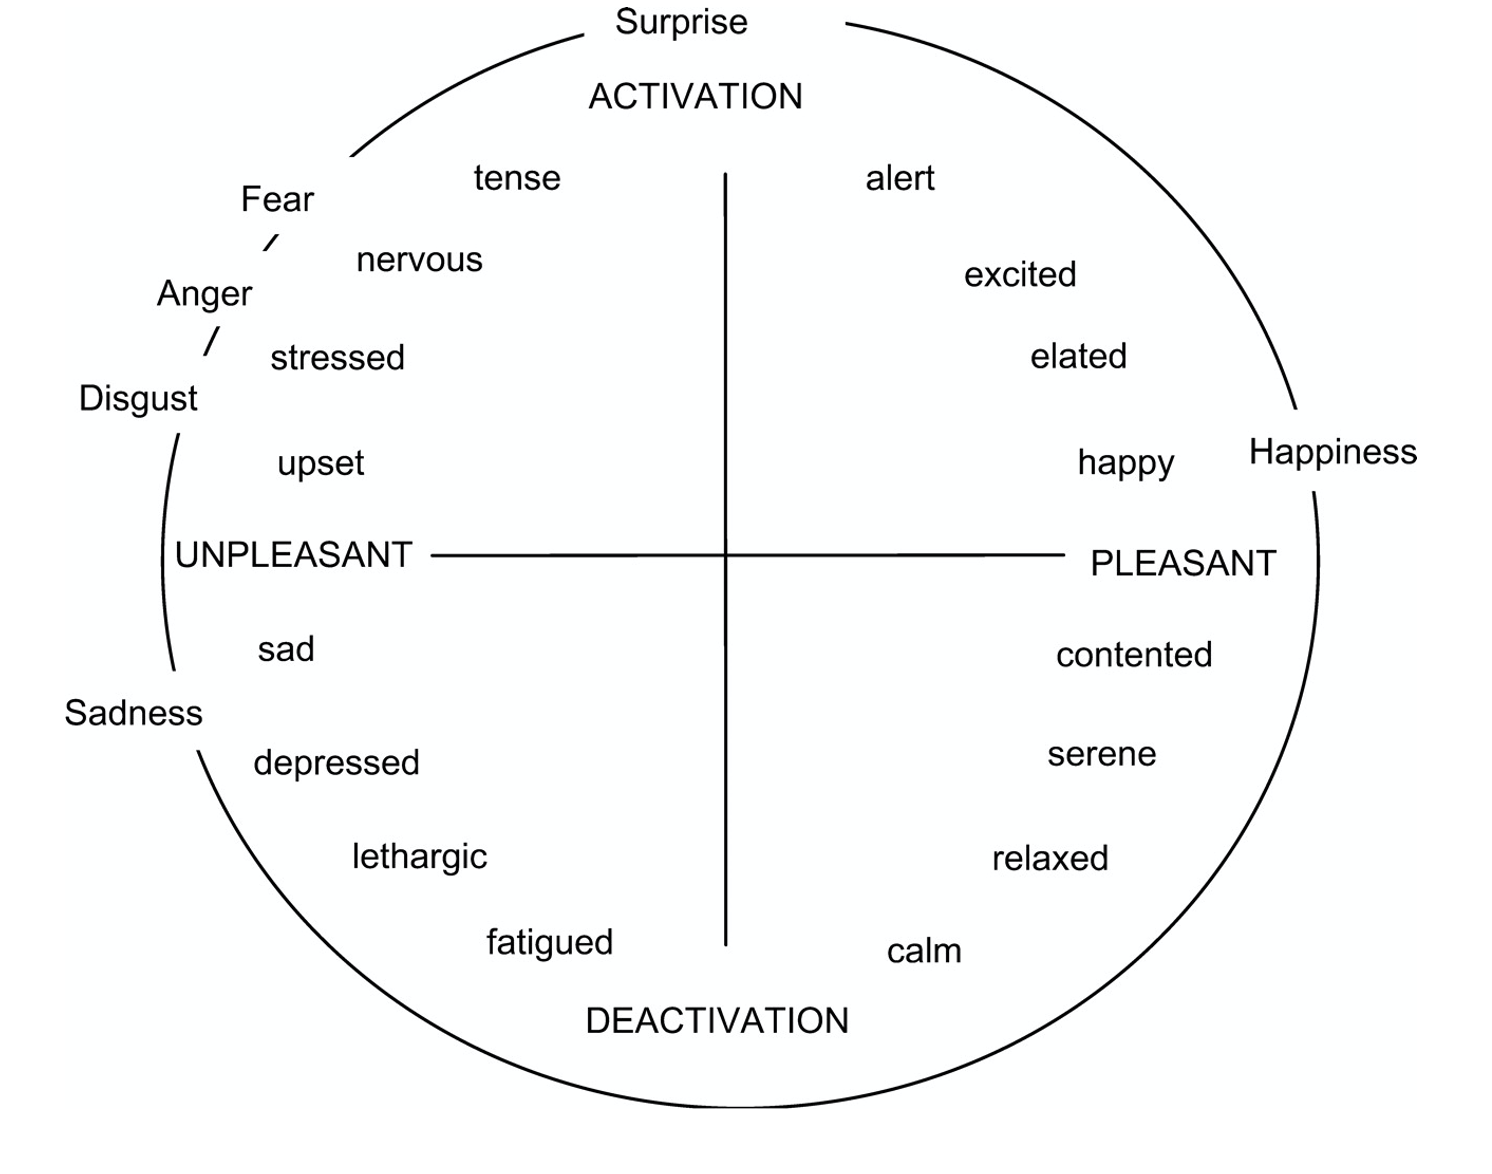
\includegraphics[scale=0.50]{images/ekmanrussel.png}
    \caption{Ekman's discrete basic emotions (outer circle) and Russell's Circumplex Model of Affect (two-dimensional plane), a reproduction from \cite{feldman1998independence}}
    \label{fig:ekmanrussel}
\end{figure}

Psychologists have developed various taxonomies, often called \textit{`models'}, for classifying emotions, ranging from universally displayed basic emotions to complex, culturally specific ones. Among these models, Ekman's basic set of emotions \citep{ekman} and Russell's circumplex model of affect \citep{russell1980circumplex} have been dominant in facial expression research, both of which can be seen in Figure \ref{fig:ekmanrussel}. \cite*{ekman1971constants} proposed six prototypical (basic) emotions, namely: anger, disgust, fear, happiness, sadness, and surprise. These emotions are universally displayed and recognised from facial expressions. This discrete model has gained popularity as it is easy for humans to recognise and describe facial expressions associated with these basic emotions. It has been the most prevalent model for measuring emotion and has dominated studies related to facial expression recognition and hence forms the basis of the emotions \textit{RTHAA} aims to classify. The alternative model proposed by Russell represents emotional states in a two-dimensional (pleasant-unpleasant, activation-deactivation) bipolar space  which is circular (similar to another popular emotion model defined by \cite{plutchik2001nature}), rather than specific discrete categories. 


\subsection{Existing Methods of Emotion Recognition}

Here, we critically compare various different methods of emotion recognition by looking at their accuracy, reliability and scalability, ultimately motivating the use of facial expression recognition and speech sentiment analysis in our work. 
\np
Emotion recognition methods can be broadly categorized into two major categories. The first category involves using internal signals, specifically physiological signals, which include the electroencephalogram (EEG), electrocardiogram (ECG), galvanic skin response (GSR) and many more. These signals are less subject to intentional control and can provide insights into the individual's internal emotional state. For example, EEG signals can capture the electrical activity in the brain, providing information about neural processes associated with certain emotions. However, collecting and analyzing physiological signals may require specialized equipment and expertise, diminishing its scalability. 
\np
Furthermore, the interpretation of the signals to recognise emotions can be complex as they use a wide variety of machine learning and deep learning models. Traditional machine learning methods require carefully designed and hand-crafted features as well as feature optimisation. Contrarily, deep learning methods learn the inherent principle of the data and extract features automatically, eliminating challenging feature engineering stages of traditional methods. The whole emotion recognition framework is shown in Figure \ref{fig:physioprocess}. Signal preprocessing, which is included both in traditional methods and deep learning methods, is adopted to eliminate the noise effects caused by the crosstalk, measuring instruments, electromagnetic interferences, etc. We will not cover the machine learning techniques employed in the processing of physiological signals, as our main focus is on the results in order to support the utilization of FER. However, we will extensively discuss the machine learning (and by extension deep learning) techniques adopted in FER.

\begin{figure}[H]
    \centering
    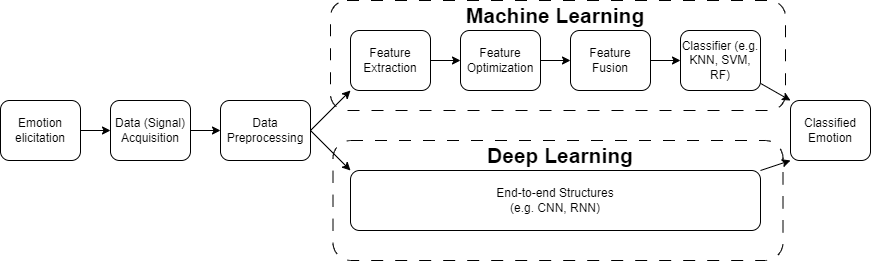
\includegraphics[scale=0.46]{diagrams/physioprocess.png}
    \caption{Emotion recognition framework using physiological signals}
    \label{fig:physioprocess}
\end{figure}

The second category involves using human physical signals, such as facial expressions \citep{7752782}, speech signals (acoustics) \citep{mao2014learning}, gestures \citep{gestures} and other overt behaviors, which are relatively easy to collect. However, the reliability of these signals may not always be guaranteed, as individuals can intentionally control their physical signals, such as masking their true emotions with a smile in a formal social setting, making it difficult to accurately identify their underlying emotions.


\subsubsection{Using Physiological Signals}

In this section, we discuss existing methods of emotion recognition that use physiological signals and how effective they are.

\paragraph{Electroencephalography (EEG)}

Electroencephalography (EEG) refers to an electrophysiological, noninvasive (does not require any surgical procedures or invasive measures) technique for the recording of electrical activity arising from the human brain. Electrodes are simply placed on the scalp, making it a relatively safe and comfortable method compared to other brain imaging techniques. \cite{wu2017estimation} provide a method for emotion recognition using only two channels of frontal EEG signals at FP1 and FP2 (the left and right frontal pole EEG electrodes) shown in Figure \ref{fig:eeg}. The experiment using a Gradient-boosting Decision Tree (GBDT) classifier validated the effectiveness of the method, where the maximum and mean classification accuracy were 76.34\% and 75.18\% respectively. Note that this method classifies signals into positive and negative (binary classification). 

\begin{figure}[H]
    \centering
    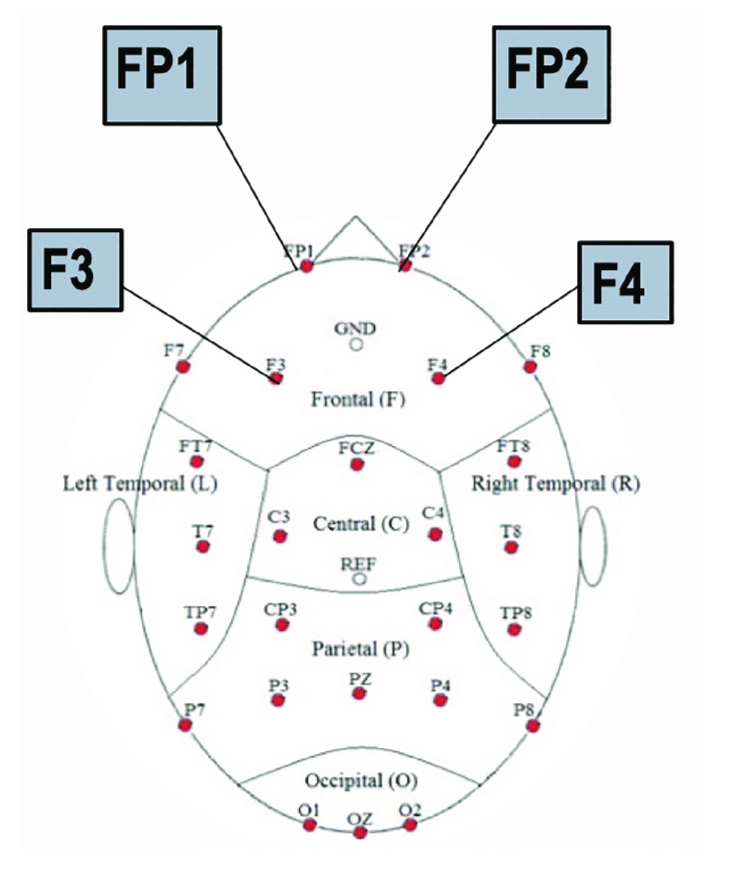
\includegraphics[scale=0.40]{images/eeg.png}
    \caption{Position of EEG electrodes on a human head, taken from \cite{neal2019discriminating}}
    \label{fig:eeg}
\end{figure}

\cite{li2018emotion} propose a new approach which considers together the temporal, spatial, and frequency characteristics of EEG signals. This approach extracts rational asymmetry (RASM) as the feature to describe the frequency-space domain characteristics of EEG signals and constructs a Long Short-Term Memory (LSTM) network as the classifier to explore the temporal correlations of EEG signals. The results showed that the mean accuracy of emotion recognition achieved 81.10\% in valence and 74.38\% in arousal (activation). While EEG achieves acceptable accuracy for binary classification tasks, current solutions cannot achieve reliable results for multi-class classification tasks, for example, attempting to classify signals into the six discrete emotions classes stated by \cite{ekman}, or to combine the readings from valence and arousal to deduce specific emotions stated in the Circumplex Model of Affect introduced by \cite{russell1980circumplex}.

\paragraph{Electrocardiography (ECG)}

Electrocardiography (ECG) refers to the noninvasive interpretation of the electrical activity of the heart in real time. Since heart activity is related with human central system ECG is useful not only in analyzing the heart's activity it can be also used successfully for emotion recognition as demonstrated by \cite{goshvarpour2017emotion}. During an ECG, small electrodes are placed on the skin of the chest, limbs, or other specific locations on the body. These electrodes are connected to a machine that records the electrical signals generated by the heart as it beats.
\np
\cite{valenza2014revealing} propose a probabilistic framework able to characterize the emotional state of a subject using a support vector machine (SVM) through the analysis of heartbeat dynamics exclusively. Results, estimating emotions each 10 seconds, achieve an overall accuracy in recognizing four emotional states (shown in Figure \ref{fig:4circum}) based on the circumplex model of affect of 79.29\%, with 79.15\% on the valence axis, and 83.55\% on the arousal axis. These results demonstrate that using ECGs for emotion recognition produce marginally more reliable results than using EEGs, however, more sources can consistently achieve results obtained by \cite{wu2017estimation} and \cite{li2018emotion} for EEGs, whereas the source cited for ECGs \citep{valenza2014revealing}, seems to be the only source that achieves higher results, causing there to be less certainty in the reliability of this source.

\begin{figure}[H]
    \centering
    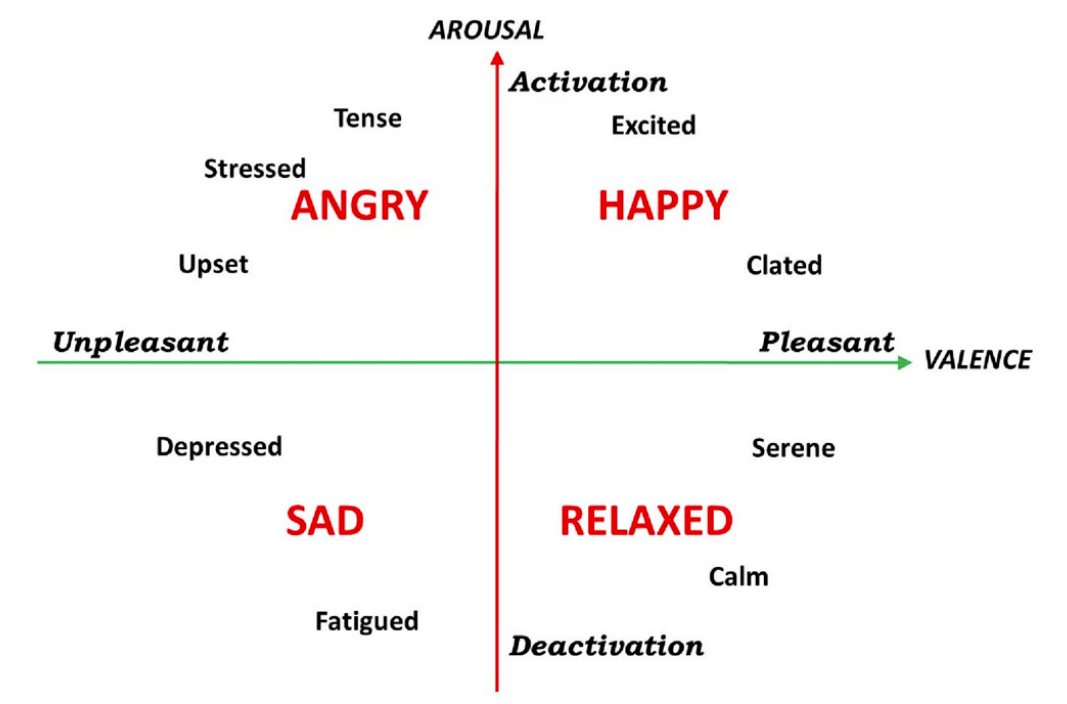
\includegraphics[scale=0.41]{images/4circum.png}
    \caption{A four-class, discrete version of Russell's Circumplex Model used in and taken from \cite{valenza2014revealing}}
    \label{fig:4circum}
\end{figure}

\paragraph{Galvanic Skin Response (GSR)}

Galvanic skin response (GSR), also known as electrodermal activity (EDA) or skin conductance (SC), refers to a physiological measurement that assesses the electrical conductance of the skin, typically on the surface of the fingers or palms, in response to emotional or physiological stimuli. GSR is commonly used as an indicator of sympathetic nervous system activity, which is associated with emotional and physiological arousal \citep{wu2010analysis, lidberg1981sympathetic}.
\np
\cite{wen2014emotion} used GSR, fingertip blood oxygen saturation and heart rate as input signals to recognise five emotions using random forests (RF). This yielded an overall accuracy rate of 74\% on a database containing 477 cases. \cite{wu2010analysis} managed to recognise six emotions with average verifying recognition rates of surprise, fear, disgust, grief, happy and angry being 78.72\%, 73.37\%, 70.48\%, 62.65\%, 62.52\% and 44.93\% respectively. \cite{das2016emotion} combined ECG and GSR signals to recognise three emotional states: happy, sad and neutral. The classification performance for happy-sad, sad-neutral and happy-neutral emotions was 93.32\%, 91.42\% and 90.12\% respectively.
\np
To summarise, the foundational notion that underpins emotion recognition using physiological signals, is that humans will respond differently according to different stimuli. Signals obtained from EEGs, ECGs, GSRs, etc. can all be used to deduce emotions. \cite{physiosignals} highlights the value of these biological responses as they are spontaneous and uncontrollable hence providing the most reliable data since they are involuntary. However, using physiological signals for emotion recognition poses some disadvantages. Firstly, subtle physical conditions, e.g. brain activity, can be influenced by external events, such as stress, so it can be difficult to ensure that any emotion induced in the person of interest is solely the cause of the environment being tested. While measures can be taken to mitigate the impact of external influences, it presents a logistical challenge if testing is desired to be done on a large number of people. Using human physical signals (e.g. facial expressions and speech) are much more scalable compared to  using physiological signals as they do not require medical expertise nor specialist equipment such as electrodes.
\np
In conclusion, the above methods manage to obtain reasonable accuracy in very controlled environments, but this accuracy begins to detoriorate considerably as more emotion classes are introduced. Using physiological signals for emotion recognition also presents logistical challenges and hence is not very scalable nor cost-effective. This motivates the central aim of this project --- to offer a more scalable and cost-effective alternative to using physiological signals by building a web application that automatically monitors emotions and sentiment accurately based on facial expressions and speech-content.


% https://www.mdpi.com/1424-8220/20/3/592#B79-sensors-20-00592

% https://www.researchgate.net/publication/339119986_Emotion_Recognition_and_Detection_Methods_A_Comprehensive_Survey

% \begin{table}[H]
% 	\centering
% 	\begin{tabular}{|p{4.2cm}|p{4.2cm}|p{4.2cm}|p{4.2cm}|}
% 		\hline
% 		\normalsize{\textbf{Emotion}} & \normalsize{\textbf{Gestures and Postures}}
%         \vspace{0.5em}
% 		\\ \hline

%         Sadness, anger, stress, surprise &
% 		\\ \hline
    
%     \end{tabular}
% 	\caption{Summary of current results of emotion recognition using physiological signals}
% 	\label{tab:physioresults}
% \end{table}


\subsubsection{Using Human Physical Signals}

\paragraph{Gestures}

\cite{gestures} show that emotion recognition can be done via the analysis of body posture (human movement). In different moods and environmental states, human beings will involuntarily undergo some posture changes as demonstrated by \cite{lee2017cepp} which can be seen in Table \ref{tab:gestureemotion}. \cite{bull2016posture, coulson2004attributing} indicate that information such as the time and frequency of these posture changes can reveal important information about the emotions a human might be feeling. However, using human gestures for emotion recognition poses certain limitations. Many gestures have little to no emotional significance, or perhaps, have different emotional meanings in different environments. Also the actual detection of gestures themselves (not the emotions they may exude) can be made extremely challenging due to image noise and hence is a hard method to generalise to all environments according to \cite{glowinski2008technique}. The combination of the factors listed above make emotion recognition via gestures inadequate if high classification accuracy is desired (unlike using facial expressions) with recently developed systems achieving a recognition rate of approximately 62\% \citep{piana2014real}.
\np
\begin{table}[H]
	\centering
	\begin{tabular}{|P{3.3cm}|p{10.2cm}|}
		\hline
		\normalsize{\textbf{Emotion}} & \normalsize{\textbf{Gestures and Postures}}
        \vspace{0.5em}
		\\ \hline

        Happiness & Body extended, shoulders up, arms lifted up or away from the body
		\\ \hline

        Interest & Lateral hand and arm movement and arm stretched out frontal
		\\ \hline

        Surprise & Right/left hand going to the head, two hands covering the cheeks self-touch two hands covering the mouth head shaking body shift-backing
		\\ \hline

        Boredom & Raising the chin (moving the head backward), collapsed body posture, and head bent sideways, covering the face with two hands
		\\ \hline

        Disgust & Shoulders forward, head downward and upper body collapsed, and arms crossed in front of the chest, hands close to the body
		\\ \hline

        Anger & Lifting the shoulder, opening and closing hand, arms stretched out frontal, pointing, and shoulders squared
		\\ \hline
    
    \end{tabular}
	\caption{Relations between emotions and body posture --- inspired by \cite{lee2017cepp, metri2011facial}}
	\label{tab:gestureemotion}
\end{table}
% \vspace{-2em}

\paragraph{Speech Signals}

Speech emotion recognition (SER) refers to the process of automatically recognizing emotions from speech signals. It involves analyzing the acoustic features of speech, such as pitch, intensity and rhythm, to identify emotional cues and infer the emotional state of the speaker. Recent carried out by \cite{ton2019speech} obtain good classification accuracies, specifically 74.31\% and 97.29\% on the German \textit{Emo-DB} and English \textit{SAVEE} databases respectively. However, individual differences combined with noisy environments can lead to significant variations in speech signals which ultimately brings some difficulties to recognition, and hence must be remediated with the use of a large phonetic database. Therefore, the acquisition of speech signals imposes strong requirements on the surrounding environment --- as stated by \cite{you2006emotion} --- similar to how background lighting can affect the discernment of emotions from facial expressions (another challenge this project aims to overcome). 
\np
In conclusion, the above methods of using human physical signals are easier to collect than the previously mentioned physiological signals, however, their accuracy depends significanly on the absence of environmental noise. This motivates the use of FER and speech sentiment analysis as they are less subject to environmental factors and have greater classification accuracies, which will be discussed in Section \ref{fer}.

\paragraph{Sentiment Analysis}
\label{bgsentanal}

Sentiment analysis is a subfield of NLP that focuses on extracting subjective information from text. For our application we look to analyse the sentiment of the user's speech by classifying their spoken words into positive, negative or neutral. We also look to employ a method that doesn't just classify into the 3 aforementioned classes, but also gives the degree to which the user's speech is positive or negative as this provides useful auxillary data. In this section we will briefly summarise some of the approaches to sentiment analysis, however, this will be explored in more detail in Section \ref{saam}.
\np
One approach to sentiment analysis is by using a lexicon-based approach. This approach uses sentiment lexicons, i.e. dictionaries, which map collections of words and phrases to an associated positive, negative, or neutral sentiment. Each word in the input text is assigned a score based on its corresponding sentiment in the lexicon, and these scores are then aggregated to calculate the overall sentiment of the text.
\np
Another approach is to use supervised machine learning models. This involves training a machine learning model on a large dataset of labelled text, where each text is labelled as positive, negative, or neutral. The model then predicts the sentiment of new, unfamiliar text. Additionally, hybrid approaches exist that combine the above approaches, such as the hybrid approach proposed by \cite{appel2018successes}.

\subsection{Facial Expression Recognition (FER)}
\label{fer}
Here, we critically compare existing machine learning and deep learning methods and models used in FER by looking at their accuracy. We will also provide a brief explanation of the functioning of each employed model where appropriate, explaining their mechanisms and operations.
\np

\begin{figure}[H]
    \centering
    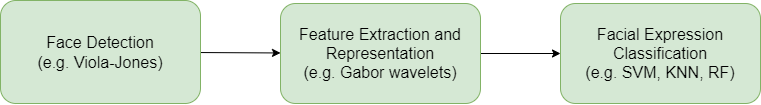
\includegraphics[scale=0.50]{diagrams/fersystem.png}
    \caption{General Design of a Facial Expression Recognition (FER) System}
    \label{fig:fersystem}
\end{figure}

FER systems can be decomposed into 3 key stages, where the output of one stage feeds into another. These stages are shown in Figure \ref{fig:fersystem} and are discussed in more detail below. 

\subsubsection{Face Detection}
\label{facedet}
The first key part of a FER system is to detect and locate human faces in the image or video. Face detection algorithms can be based on various techniques including Viola-Jones algorithm \citep{viola2001rapid} and Multi-task Cascaded Convolutional Networks (MTCNN) \citep{xiang2017joint}. The Viola-Jones algorithm  works by scanning an image using a sliding window and classifying each sub-window as either containing an object of interest or not. MTCNN is a deep learning-based algorithm that consists of three stages of deep neural networks that work in a cascading manner to detect faces in an image. These algorithms typically output the coordinates of the bounding boxes around the detected faces. \cite{vaillant1994original} designed one of the first neural networks for face localization without making any assumptions about the position, scale, or background of the face. Scale independence was achieved by scanning the input window at multiple scales. Since then, convolutional neural networks (CNNs) that use cascading approaches have become more popular \citep{li2015convolutional, xiang2017joint}. Commonly used datasets for model training and testing include Annotated Facial Landmarks in the Wild (AFLW) \citep{koestinger2011annotated}, WIDER FACE \citep{yang2016wider} and Labeled Faces in the Wild (LFW) \citep{huang2008labeled}. \cite{farfade2015multi} fine-tune an AlexNet --- a CNN architecture --- and show state-of-the-art results on the AFLW dataset which has faces with varying levels of rotation, illumination and occlusion. To summarise, deep learning approaches lead in performance, specifically, \cite{jiang2017face} demonstrate that CNNs are currently the best algorithms used in face detection, compared to traditional algorithms such as Viola-Jones achieving state-of-the-art results on the WIDER FACE test set as well as other face detection benchmarks such as The Face Detection Data Set and Benchmark (FDDB) \citep{fddbTech}.

\subsubsection{Feature Extraction and Representation (Selection)}

The next stage involves extracting a forming the correct representation of a face. Feature extraction involves extracting meaningful features from the detected faces that can be used as inputs for the expression recognition algorithm. These features could include facial landmarks, facial action units or texture information. One such algorithm for extracting meaningful features is principal component analysis (PCA), a latent factor model which transforms the original features of the data into a new set of orthogonal features called principal components, which are linear combinations of the original features. The principal components capture the most important patterns or structures in the data.
\np
Afterwards, we must select some of the extracted features to choose in our final feature representation, this process is known as feature reduction, sometimes called dimensionality reduction. The extracted features may be high-dimensional and not all features may be relevant for expression recognition. Feature selection techniques may be applied to select the most informative features that contribute to accurate expression recognition. PCA can be used for dimensionality reduction which can reduce the computational burden of once-difficult tasks. This is done by selecting a specified number of top principal components \textit{k}, which help obtain the most important features. $k$ is a hyper-parameter that should be tuned via techniques such as $K$-fold cross-validation. PCA is often performed by using singular value decomposition (SVD) which computes $d$ eigenvectors (principal components) where $d$ is the number of features of the dataset. These eigenvectors have the same dimensionality as the original feature vectors themselves and hence can be re-arranged as matrices, commonly known as `eigenfaces' in the field of facial image analysis, as seen in Figure \ref{fig:eigenfaces}, along with the original dataset shown in Figure \ref{fig:presidents}:

\begin{figure}[H]
    \centering
    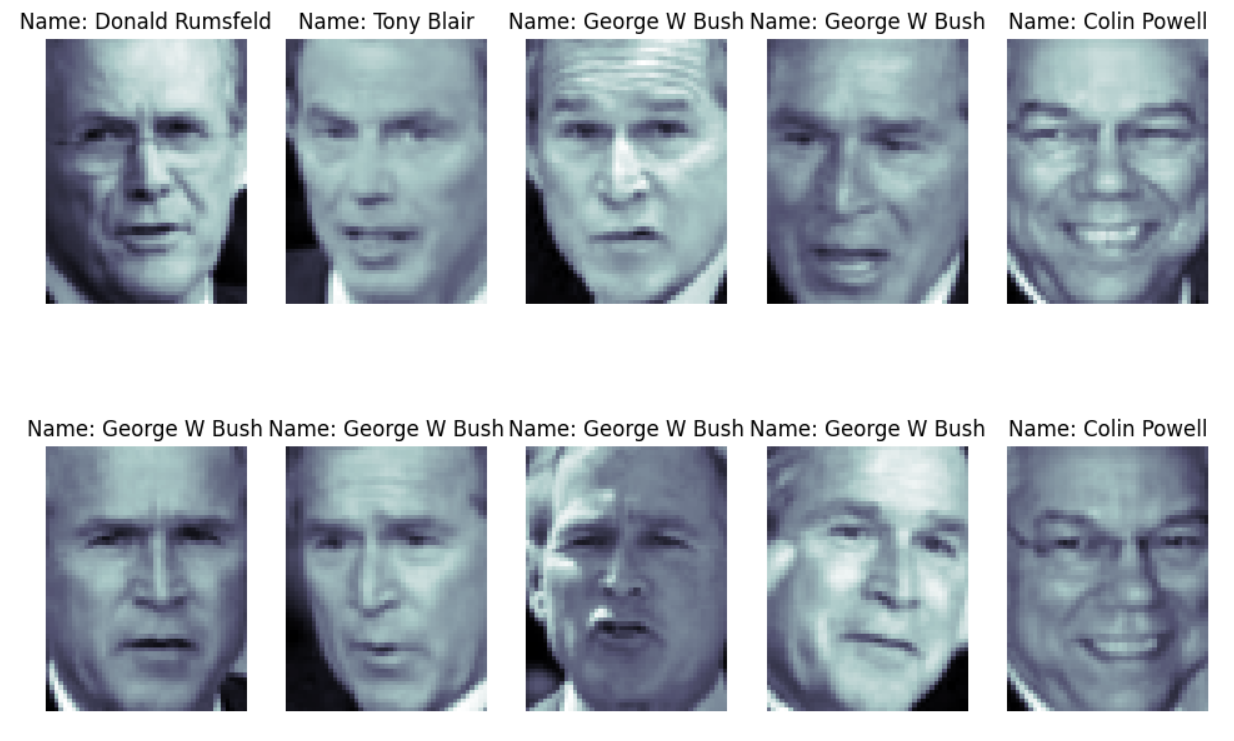
\includegraphics[scale=0.55]{images/presidents.png}
    \caption{\textit{Labeled Faces in the Wild (LFW)} dataset containing images of famous political figures}
    \label{fig:presidents}
\end{figure}

\begin{figure}[H]
    \centering
    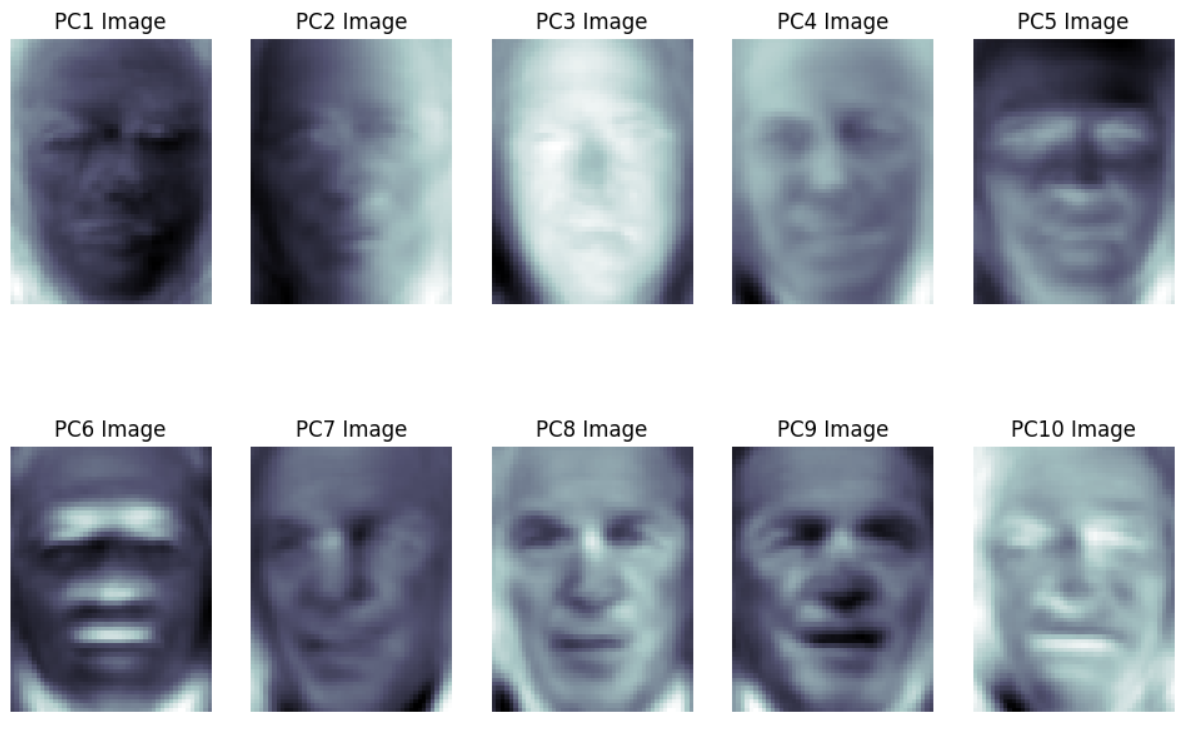
\includegraphics[scale=0.55]{images/eigenfaces.png}
    \caption{Principal Components (PCs)/Eigenfaces of the \textit{LFW} dataset shown as images}
    \label{fig:eigenfaces}
\end{figure}

Dimensionality reduction is usually a lossy conversion (information is lost) but PCA is a strong technique to alleviate that information loss. It allows for the removal of redundant information, and variations that can drastically improve the classifiability of data, such as kernel-based PCA, will likely be used prior to the classification phase of the FER system (however this usually comes at the cost of projecting onto high-dimensional feature spaces, which has performance implications).

\subsubsection{Facial Expression Classification}
\label{ferrr}
\np
Finally, we select a model to classify the facial expressions that are represented in our feature space. The model is trained on the labelled dataset, which now includes the detected face images with expression labels, to learn the patterns of different expressions. Below, we outline some of the widely-used datasets as well as the most popular machine learning and deep learning methods used in FER and their results on these datasets.

\paragraph{Datasets}
\label{datasets}
Listed below are the datasets that are commonly used in the training and evaluation of models in FER and are considered the benchmark datasets:

\begin{itemize}
    \item \textbf{The Extended Cohn-Kanade (CK+) Dataset} \citep{lucey2010extended} \\ The CK+ dataset contains grayscale images (a sample of which can be seen in Figure \ref{fig:ckds}) of both male and female people for eight emotions (69\% female). The CK+ dataset contains the facial expressions of 210 adults with ages ranging from 18 to 50 years, among them 81\% Euro-American, 13\% Afro-American, and 6\% diverse groups. Unfortunately, the CK+ dataset contains an uneven number of samples for each emotion class (as shown in Figure \ref{fig:ckeda}), lending itself vulnerable to overfitting. 
    \np
    \begin{figure}[H]
        \centering
        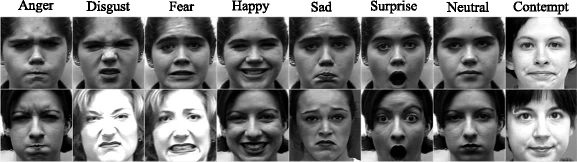
\includegraphics[scale=1]{images/ck.png}
        \caption{Preprocessed sample images of CK+ dataset from \cite{kar2019face}}
        \label{fig:ckds}
    \end{figure}
    
    \begin{figure}[H]
        \centering
        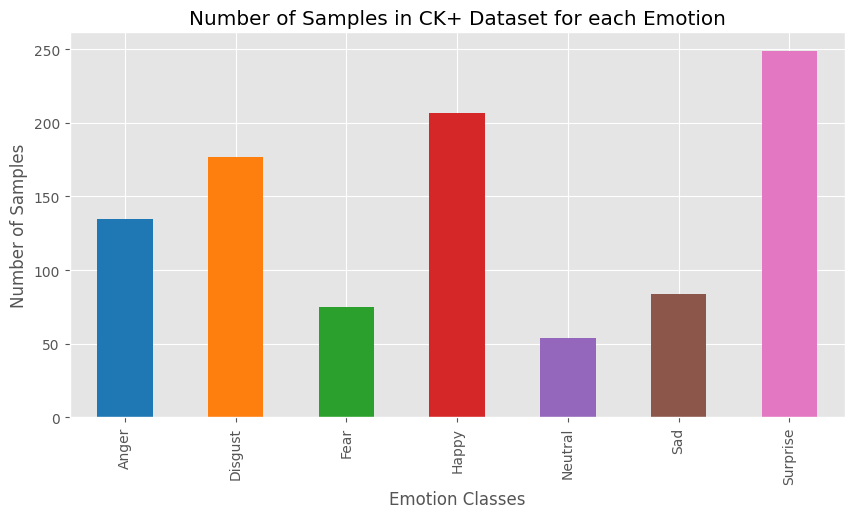
\includegraphics[scale=0.60]{images/ckeda.png}
        \caption{Number of samples for each emotion class in the CK+ dataset}
        \label{fig:ckeda}
    \end{figure}

    \item \textbf{Japanese female facial expression (JAFFE) Dataset} \citep{lyons1998coding} \\ The JAFFE dataset contains 213 grayscale images (a sample of which can be seen in Figure \ref{fig:jaffe}) taken from 10 subjects, each exhibiting seven different emotions including happiness, neutral, sadness, anger, disgust, contempt, fear and surprise. Each emotion label has approximately the same number of images associated with it (29-31 images), mitigating the chance of overfitting. Within the dataset, each subject has a minimum of 3-4 images for each emotion label.
    \np
    
    \begin{figure}[H]
        \centering
        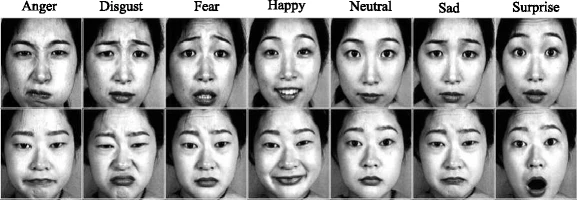
\includegraphics[scale=1]{images/jaffe.png}
        \caption{Preprocessed sample images of JAFFE dataset from \cite{kar2019face}}
        \label{fig:jaffe}
    \end{figure}

    \item \textbf{AffectNet Dataset} \citep{mollahosseini2017affectnet} \\
    The AffectNet dataset includes over 1,000,00 coloured images of faces that were gathered from the internet using 1250 emotion-related keywords in six different languages, by querying three major search engines. Consequently, it is the largest database of facial expressions, valence, and arousal, allowing the use of two different emotion models (taxonomies): a categorical model similar to the one introduced by \cite{ekman}, and continuous (dimensional) model, similar to the one developed by \cite{russell1980circumplex}. Unfortunately, AffectNet suffers from an uneven distribution of images for each emotion category as shown in Table \ref{tab:an}, which can lead to overfitting.

    \begin{table}[H]
        \centering
        \begin{tabular}{|P{3.5cm}|p{9.2cm}|}
            \hline
            \normalsize{\textbf{Category}} & \normalsize{\textbf{Total number of manually annotated images in the training and validation set}}
            \vspace{0.5em}
            \\ \hline
            Neutral     &   75374    \\ \hline
            Happy       &   134915 \\ \hline
            Sad         &   25959 \\ \hline
            Surprise    &   14590 \\ \hline
            Fear        &   6878 \\ \hline
            Disgust     &   4303 \\ \hline
            Anger       &   25382 \\ \hline
            Contempt    &   4250 \\ \hline
            None        &   33588 \\ \hline
            Uncertain   &   12145 \\ \hline
            Non-Face    &   82915 \\ \hline
            Total       &   420299 \\ \hline

        \end{tabular}
        \caption{The total number of manually annotated images in the training and validation set (excluding test set) in each category of emotion in the AffectNet dataset}
        \label{tab:an}
    \end{table}

    \item \textbf{FER-2013 Dataset} \citep{goodfellow2013challenges} \\ The Facial Expression Recognition 2013 dataset contains approximately 30,000 facial RGB images of different expressions of which there are seven: angry, disgust, fear, happy, sad, surprise and neutral. FER-2013 also suffers from an uneven distribution of images for each emotion label, specifically, there are significantly less images for \textit{disgust} than there are for \textit{happy} as demonstrated by Figure \ref{fig:fereda}, allowing the potential for any model trained on this dataset to underfit on \textit{disgust} and overfit on \textit{happy}.
    \np
    \begin{figure}[H]
        \centering
        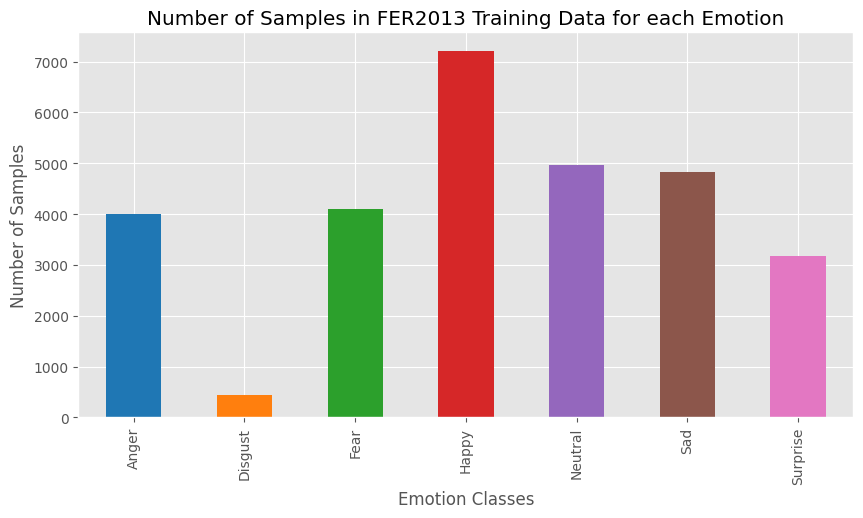
\includegraphics[scale=0.60]{images/fereda.png}
        \caption{Number of samples in training set for each emotion class in the FER-2013 dataset}
        \label{fig:fereda}
    \end{figure}

\end{itemize}

More information about each dataset can be found in the ZIP file submitted along with this report. The ZIP contains an exploratory data analysis (EDA) of the datasets mentioned above (where Figures \ref{fig:ckeda} and \ref{fig:fereda} were obtained from).


% Machine Learning - SVMs, Decision Trees / RFs, K-NN

% Deep learning - CNN, RNN, MLP, LSTM, GAN

\paragraph{Support Vector Machines}

Support vector machines (SVMs) are one of the earliest, simplest and most popular techniques used in machine learning. They are supervised learning models that are principally used in regression and classification problems. The main idea behind SVMs is to find the best possible decision boundary (or hyperplane) that maximises the margin seperating the data points of different classes --- the margin being defined as the distance between the hyperplane and the nearest data point of each class as shown in Figure \ref{fig:svm}.

\begin{figure}[H]
    \centering
    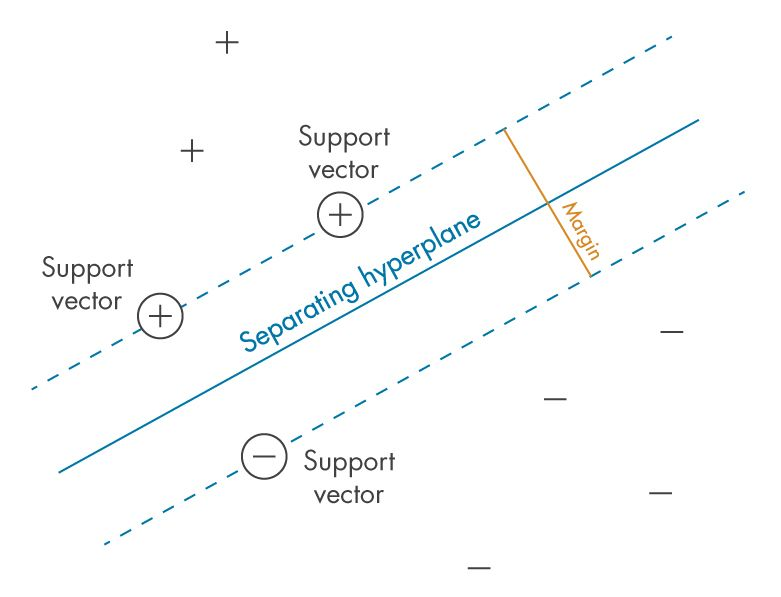
\includegraphics[scale=0.53]{images/svm.jpg}
    \caption{Support vector machine that classifies data points belonging to two classes: positive (+) and negative (-). Image taken from \cite{svmimage}}
    \label{fig:svm}
\end{figure}

One of the earlist methods that use SVMs was proposed by \cite{michel2003real} in the detection of facial expressions in live videos. Features are extracted using a facial tracker and are then classified using a SVM. \cite{kazmi2012wavelets} use a wavelets based method in which the classification is done by using seven SVMs in parallel. Each SVM classifies one expression which is later aggregated with others using a maximum function, achieving a classification accuracy of 81.57\% on the JAFFE dataset. The approach proposed by \cite{zhang2015facial} utilizes multiple kernel learning (MKL) in SVMs to combine features. In this method, the calculation of kernel weights is performed sequentially within the SVM, taking into consideration both sparse and non-sparse kernel combinations, achieving an accuracy of 93.6\% on the CK+ dataset. Most recently, \cite{kar2019face} propose a scheme that works in three stages. The first stage employs ripplet transform type II (ripplet-II) to extract features from facial images because of its efficiency in representing edges and textures. The next stage uses PCA and linear discriminant analysis (LDA) to obtain a more compact and discriminative feature set. In the final stage, classification is performed using a least squares variant of SVMs (LS-SVM) with a radial basis function (RBF) kernel. The proposed system is validated on the CK+ and JAFFE datasets, achieving accuracies of 98.97\% and 99.46\% respectively yielding superior performance compared to other state-of-the-art schemes.

\paragraph{$K$-Nearest Neighbors}

$K$-nearest neighbors ($K$-NN) classifiers are another widely-used classifier in emotion recognition and machine learning more generally. It is a supervised, non-parametric (size of the model grows with input data size) model used for classification tasks. $K$-NN classifiers are based on the Lipschitzness assumption:

\begin{tcolorbox}[colback=red!5!white,colframe=red!50!black,title=Lipschitzness Assumption]
If two feature vectors are close to each other, then their classes are likely to be the same.
\end{tcolorbox}

When attempting to classify new, unlabeled data points, the $K$-NN algorithm calculates the distance (similarity) between the new data point and the reference set of training data points. The $K$-NN algorithm then selects the $k$-nearest neighbors --- the $k$ training data points that are closest in terms of similarity to the new data point. The most frequent class in these $k$-nearest data points is assigned to the unlabeled data point.
\np
\cite{dino2019facial} present a system which classifies images into eight basic facial expressions which are normal, happy, angry, contempt, surprise, sad, fear and disgust. This method uses the Viola-Jones algorithm \citep{viola2001rapid} for face detection and histogram of oriented gradients (HOG) is used as a descriptor for feature extraction from the images of expressive faces. HOG is a feature extraction technique that works by computing local gradient information from an image to create histograms that represent the distribution of gradient orientations in different regions of the image and intern captures local edge information. PCA is applied for the purpose of dimensionality reduction. Finally, a $K$-NN classifier is used for classification, resulting in an accuracy of 79.97\% on the CK+ dataset. Another method that employs a similar approach by using a modified Viola-Jones algorithm and $K$-NN classifier proposed by \cite{yadav2020facial} achieves a classification accuracy of 98.5\% and 95.15\% on the JAFFE and CK+ datasets respectively. This method differs in the way that it uses a hybrid approach that combines two features, namely HOG and local binary pattern (LBP), which are used for feature extraction.

\paragraph{Random forest}

Random forests (RF) are an ensemble learning method in machine learning that use multiple decision trees (tree-like structures used for making decisions) to make predictions. During training, multiple trees are trained on random subsets of the data and features. During prediction, the predictions from all the trees are combined to obtain the final prediction. \cite{pu2015facial} propose a framework that uses a twofold random forest (i.e. two distinct random forests), resulting in a classification accuracy of 96.38\% on the CK+ dataset. \cite{munasinghe2018facial} proposes a method that uses facial landmarks which uses HOG for feature extraction and a sliding window detection scheme for detecting faces. The resulting accuracy achieved was 90\% on the CK+ dataset.

\paragraph{Neural Networks}

We now explain the notion of a neural network, as this forms essential domain knowledge needed to understand the proceeding models used in FER. Neural networks, commonly referred to as artificial neural networks (ANNs), are a class of computational models used in machine learning that are inspired by the human brain. Neural networks refer to a class of machine learning algorithms that are designed to learn patterns from data in an adaptive and hierarchical manner. Neural networks consist of nodes that are interconnected (also called neurons) and are organised into layers that are typically stacked on top of each other to form a network as shown in Figure \ref{fig:nnexample}. 
\np
\begin{figure}[H]
    \centering
    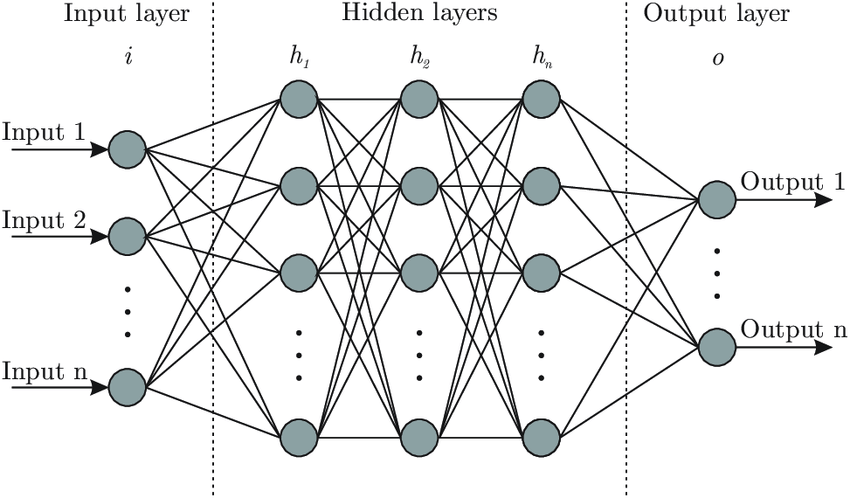
\includegraphics[scale=0.40]{images/nnexample.png}
    \caption{Example of an artificial neural network, taken from \cite{nnexample}}
    \label{fig:nnexample}
\end{figure}

Neural networks consist of three main types of layers: the input layer, hidden layers, and output layer. The input layer receives the input data, which can be in a variety of forms (images, text, etc.), and is represented as nodes. The hidden layers process and transform the input data to learn relevant features or representations, and typically consist of multiple nodes. The number of hidden layers and nodes in each hidden layer can vary. The output layer (the final layer of the neural network) produces the output based on the learned representations. Another crucial part of neural networks are the connections between the nodes which are represented by weighted edges, which transmit information from one layer to another. While the neural network is being trained, the weights are adjusted according to a learning algorithm e.g. stochastic gradient descent (SGD). This is done iteratively to minimise the error between the predicted output and the actual output, allowing the network to learn and improve its performance.

\paragraph{Multi-layer perceptrons}

A multi-layer perceptron (MLP) is a type of ANN used in machine learning for supervised learning tasks such as classification and regression. Information flows in one direction from the input layer through the hidden layers to the output layer. \cite{dino2019facial} uses a MLP to achieve a classification accuracy of 82.97\% on the CK+ dataset. This method uses the Viola-Jones algorithm \citep{viola2001rapid} for face detection as well as HOG and PCA for feature representation (before finally being classified by a MLP). \cite{boughrara2016facial} propose a method that achieves 84.58\% and 96.66\% on the FER-2013 and CK+ datasets respectively.

\paragraph{Convolutional Neural Networks}

Convolutional neural networks (CNNs) refer to a deep learning model that are designed to automatically learn and extract relevant features from input data, making them well-suited for tasks that require understanding and processing visual patterns i.e. they have been explicitly designed to work well with images.  This is due to their ability to extract multiple layers of abstract representations, for example, the first convolutional layer might be responsible for edge or corner detection, whereas the last convolutional layer is responsible for detecting more complex patterns, a face, for example (see Figure \ref{fig:cnnfe}). Convolutional layers perform convolution operations, which involve applying filters to input data (images in our case) in a sliding window fashion, to extract local patterns or features. Convolutional layers are typically followed by activation functions (e.g. ReLU, sigmoid, etc.) to introduce nonlinearity into the model. Poolinglayers are introduced to help reduce computational complexity (by downsampling the feature maps generated by the convolutional layers) and improve the model's ability to generalise across different spatial locations. Lastly, some layers in the network may have dropout --- a regularization technique used to prevent overfitting by randomly setting a fraction of the neurons to zero during training, forcing the network to learn more robust representations.

\begin{figure}[H]
    \centering
    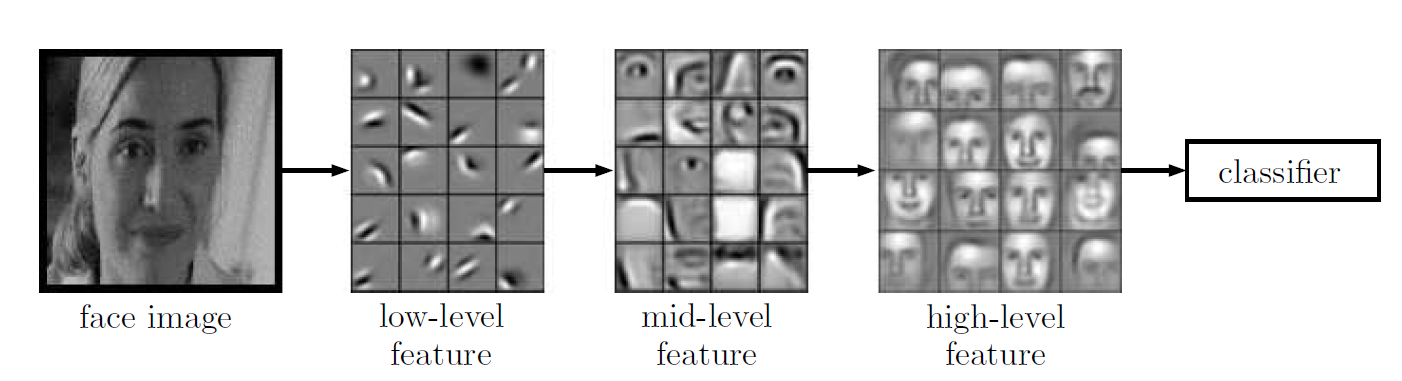
\includegraphics[scale=0.50]{images/cnnfe.png}
    \caption{Hierarchical features in CNNs, taken from \cite{nguyen2019facial}}
    \label{fig:cnnfe}
\end{figure}

\begin{figure}[H]
    \centering
    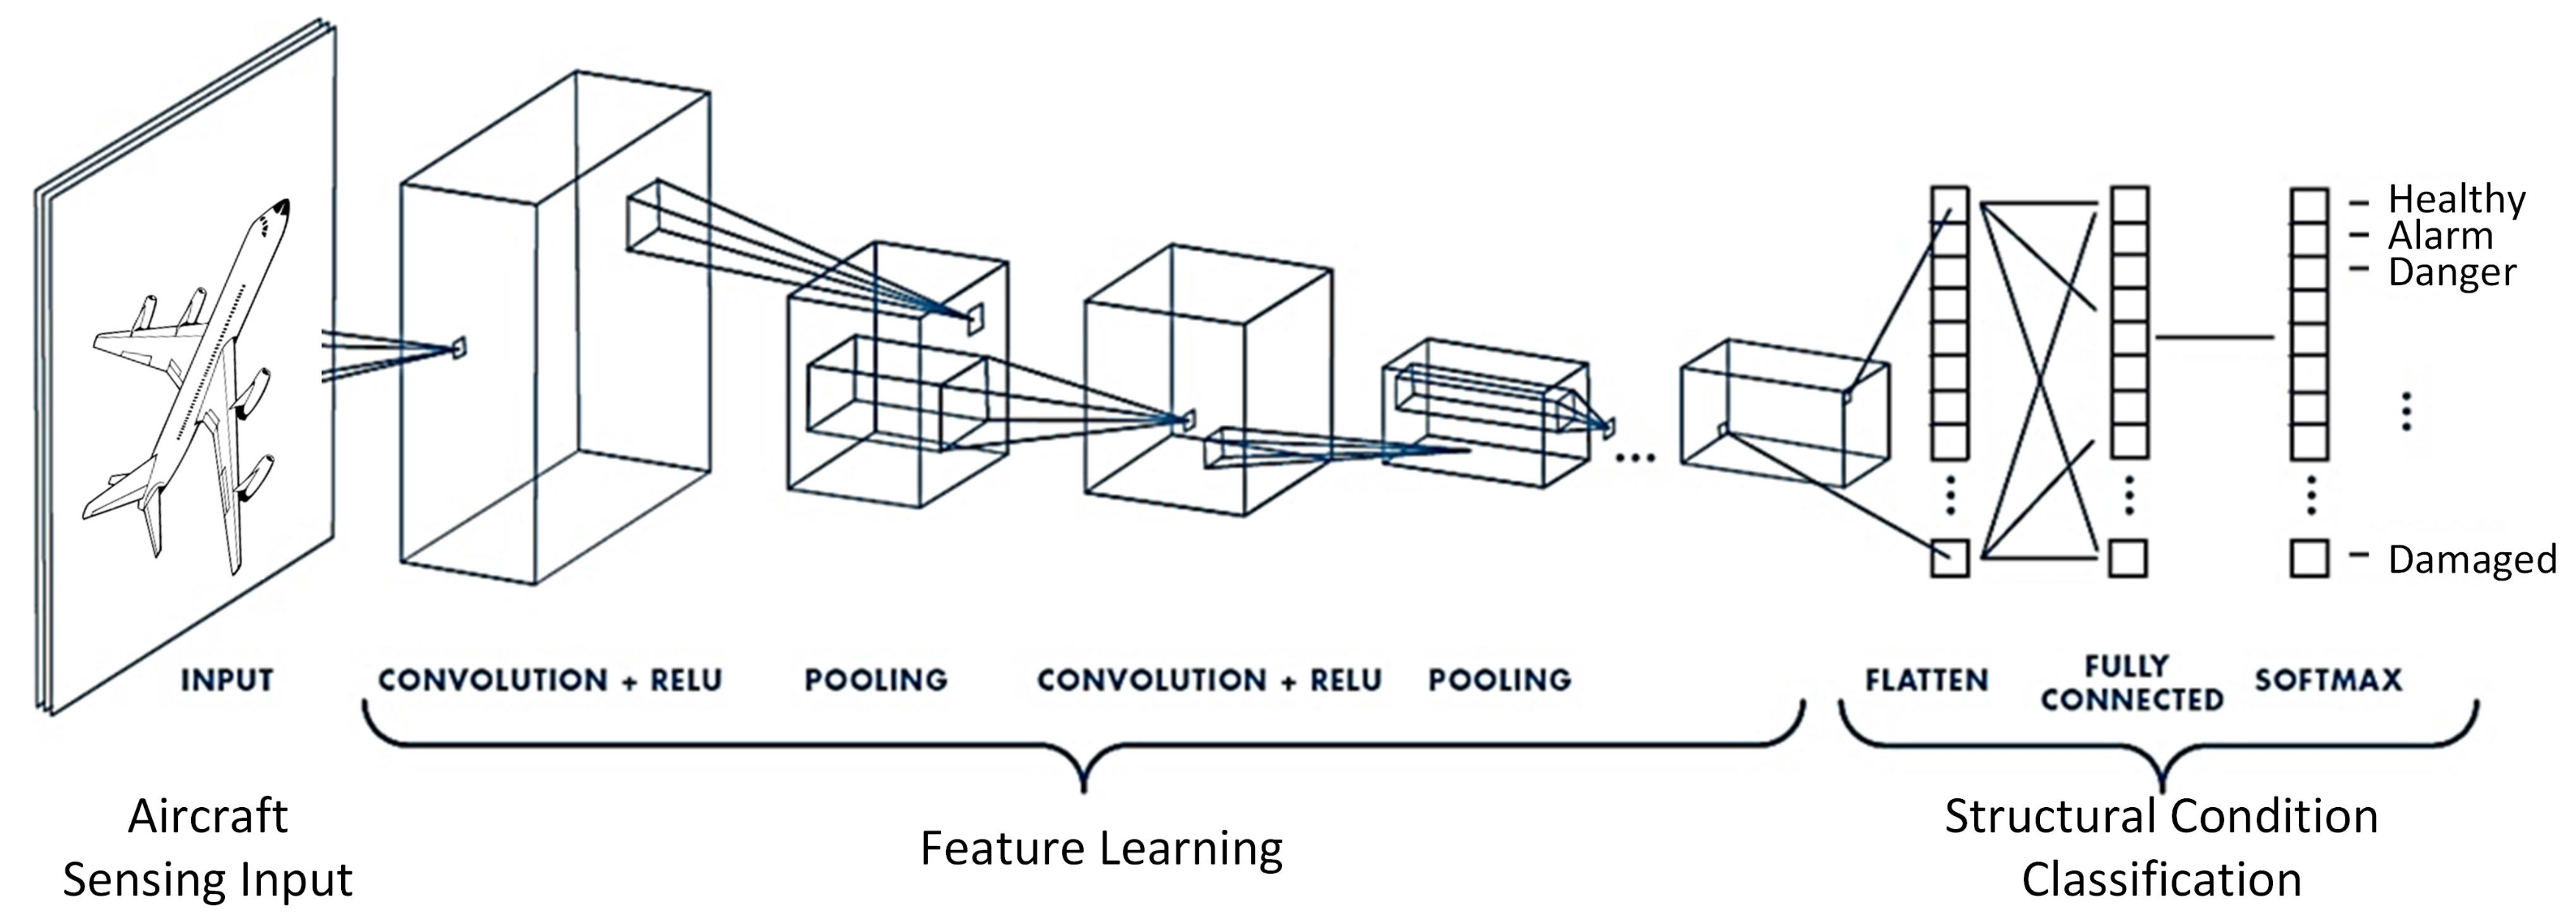
\includegraphics[scale=0.16]{images/cnn.png}
    \caption{Generic architecture of a CNN, taken from \cite{tabian2019convolutional}}
    \label{fig:genericcnn}
\end{figure}

\cite{xie2017facial} propose a feature redundancy-reduced convolutional neural network (FRR-CNN) which is a variant of the traditional CNN architecture that results in less redundant features being generated during feature extraction, yielding a more compact representation of an image. This leads to a more efficient and effective deep learning model. This CNN aims to classify images into the taxonomy introduced by \cite{ekman}, and achieves an accuracy of 92.06\% on the CK+ dataset. Table \ref{tab:confmatrix} shows the confusion matrix of the FRR-CNN on the CK+ dataset. 

\begin{table}[H]
	\centering
	\begin{tabular}{|P{3.5cm}|P{1.2cm}|P{1.2cm}|P{1.2cm}|P{1.2cm}|P{1.2cm}|P{1.2cm}|}
		\hline
		Predicted Label $\rightarrow$ Actual Label $\downarrow$ & \normalsize{\textbf{AN}} & \normalsize{\textbf{SA}} & \normalsize{\textbf{HA}} & \normalsize{\textbf{DI}} & \normalsize{\textbf{FE}} & \normalsize{\textbf{SU}}
		\\ \hline

        \textbf{AN}	& 86.11 & 11.11 &	0	& 2.78	& 0	&0\\ \hline
        \textbf{SA}	& 23.46	&69.14&	0&	3.70	&0	&3.70\\ \hline
        \textbf{HA}	& 0	& 0	&95.06	&2.47	&2.47	&0\\ \hline
        \textbf{DI}	& 3.09	&0	&1.85	&95.06	&0	&0\\ \hline
        \textbf{FE}	& 16.67&	0	&1.85	&0	&75.93	&5.56\\ \hline
        \textbf{SU}	& 0&	0&	0	&0	&0	&100\\ \hline
    
    \end{tabular}
	\caption{Normalised confusion matrix of FRR-CNN on CK+ dataset (\%) used in \cite{xie2017facial} where AN, SA, HA, DI, FE and SU correspond to anger, sadness, happiness, disgust, fear and surprise respectively}
	\label{tab:confmatrix}
\end{table}

\cite{li2018occlusion} propose a CNN architecture that achieves an accuracy of 97.03\% on the CK+ dataset. The CNN proposed also attempts to cope with occlusions in images as well, achieving an impressive accuracy of 54.84\% on the modified AffectNet dataset (modified to include occlusions in each image), the congusion matrix of which can be seen in Figure \ref{fig:anconfmatrix}. 

\begin{figure}[H]
    \centering
    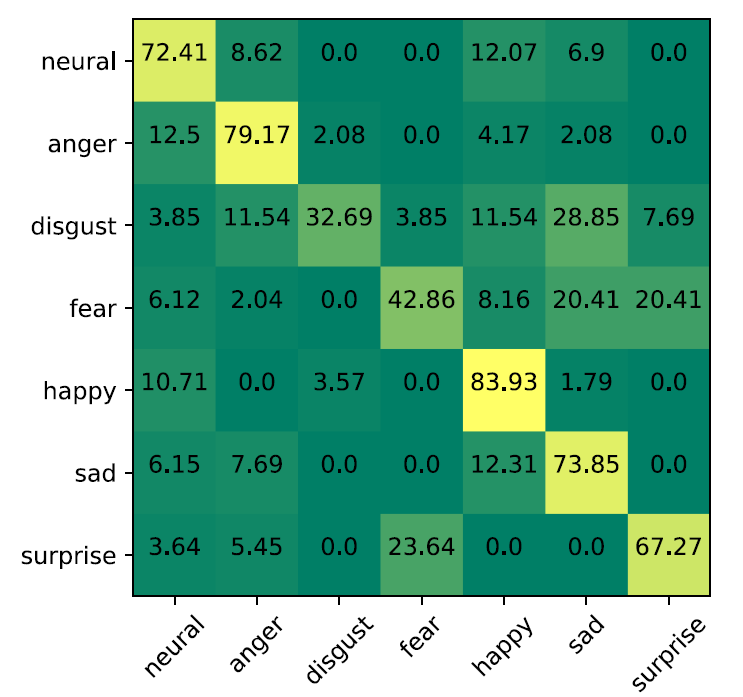
\includegraphics[scale=0.55]{images/anconfmatrix.png}
    \caption{Normalised confusion matrix of CNN proposed by \cite{li2018occlusion} on AffectNet (merged with Real-world Affective Faces (RAF-DB) dataset)}
    \label{fig:anconfmatrix}
\end{figure}

Table \ref{tab:fersummary} summarises the discussion above and shows that, deep learning approaches generally perform marginally better on CK+ (the most common benchmark dataset used in almost all the methods discussed, and hence most appropriate to compare with) unless computationally expensive feature extraction techniques, such as ripplet-II transform, are used before classification. As a result, we will be leaning more to utilising deep learning approaches in our application as they achieve a good balance of classification accuracy and also computational cost. Since our application we want to develop must classify faces in real-time, ensuring our model is fast is an important consideration.

\begin{table}[H]
    \centering
    \begin{tabular}{|L{3.5cm}|L{2.7cm}|L{3cm}|L{3.5cm}|}
        \hline
        \normalsize{\textbf{Method}} & \normalsize{\textbf{Dataset}} & \normalsize{\textbf{Accuracy (\%)}} & \normalsize{\textbf{Reference}}
        \vspace{0.5em}
        \\ \hline

        SVM (wavelets)    &   JAFFE    &   81.57   &  \cite{kazmi2012wavelets}  \\ \hline
        SVM (MKL)    &   CK+    &   93.60   &  \cite{zhang2015facial}  \\ \hline
        SVM (ripplet-II)   &   CK+, JAFFE    &   98.97, 99.46   &  \cite{kar2019face}  \\ \hline
        $K$-NN (Viola-Jones)    &   CK+    &   79.97   &  \cite{dino2019facial}  \\ \hline
        RF (twofold)    &   CK+    &   96.38   &  \cite{pu2015facial}  \\ \hline
        RF (HOG)   &   CK+    &   90   &  \cite{munasinghe2018facial}  \\ \hline
        MLP    &   CK+    &   82.97  &  \cite{dino2019facial}  \\ \hline
        MLP    &   CK+, FER-2013    &   96.66, 84.58   &  \cite{boughrara2016facial}  \\ \hline
        CNN    &   CK+    &   92.06   &  \cite{xie2017facial}  \\ \hline
        CNN    &   CK+, AffectNet (with occlusions)    &   97.03, 54.84   &  \cite{li2018occlusion}  \\ \hline

    \end{tabular}
    \caption{Summary of the main methods used in FER and their results on widely-used datasets}
    \label{tab:fersummary}
\end{table}



% Emotion recognition has many applications ...

% Mention:

% Applications of a such a tool??

\subsection{Application Development and User Interface Design}
\label{adduid}
% Why website > mobile app + desktop app

This section of the report is going to explore the ways a tool like \textit{RTHAA} could be possibly be developed. We will justify why a web application is more suitable than a desktop application or a mobile application for our use case.  We will also briefly discuss some of the common considerations when it comes to user interface design in relation to web application development.
\np
% We will also briefly discuss some of the main technologies available for web development and what is most suitable for our work. This will be discussed further in the design section of the report 
Web applications offer many advantages compared to desktop applications and mobile applications, the most notable of which is its accessibility. Since our application will be used for usability testing, we want to be able to use it on as many devices as possible to allow the user the greatest flexibility in how and what they can test. Web applications can be accessed through web browsers on a wide range of devices such as desktop computers, laptops, tablets and smartphones without the need for installing any software locally. This ultimately makes web applications more accessible as they can be accessed from anywhere with an internet connection and a compatible web browser. Furthermore, web applications are easier to update and maintain from the user's perspective as they can access the latest version of the application without needing to manually update software on their local devices that also takes up local memory on their device.
\np
However, web applications do pose certain limitations that neither desktop nor mobile applications pose. Web applications tend to have greater performance limitations as they run in web browsers and are subject to browser constraints and are reliant on the user's internet connection. They may also have limited offline functionality, as they require an internet connection to be accessed. Additionally, web applications may have security considerations, as they are accessible over the internet and may be vulnerable to web-based attacks. Despite these limitations, our application remains unhindered as it processes everything locally on the user's device, meaning that once the page has loaded, users will not necessarily need an internet connection to be able to use the application as everything happens in the user's browser and requires no further communication with a remote server.
\np
User interface (UI) design in web development entails creating visual and interactive elements for users to interact with effectively and efficiently. A primary consideration in the design of user interfaces in web applications is accessibility for users with disabilities, such as visual or hearing impairments. We will be looking to follow accessibility guidelines and standards, such as the Web Content Accessibility Guidelines (WCAG) developed by the \cite{WCAG21}. This helps ensure that the interface is inclusive and can be used by all users. Widely-used UI design principles such as Nielsen's usability principles \citep{nielsen1994usability}, will also be employed where appropriate as they provide a framework for evaluation and help avoid common mistakes that can negatively impact the user experience. UI design will be discussed in greater detail in Section \ref{design} of this report.

\subsection{Existing Solutions}
\label{es}

Affective computing (automated emotion recognition) is a relatively nascent field, consequently resulting in only a few number of tools being available large number of tools exist for human attribute analysis, the most popular of which include: \cite{noldus}, \cite{morphcast} and \cite{imotions}. We will discuss the strengths and weaknesses of each tool and how our work improves on these tools, forming the objectives of this project.

\subsubsection{Noldus}

\textit{Noldus Information Technology} is a company specializing in behavioral research and data analysis. Their facial expression recognition software is known as \textit{FaceReader}. \textit{FaceReader} is a unimodal web application tool that works via image upload and hence is incapable of real-time analytics, therefore being more restricted in its use cases. However, the tool is capable of predicting other human attributes such as age and sex. Figure \ref{fig:essnoldus} in Appendix \ref{appendix:ess} shows a screenshot of Noldus' \textit{FaceReader}.

\subsubsection{MorphCast}

\textit{Morphcast} have developed a unimodal client-side (i.e. works entirely in the browser) web application. Making the application client-side is more preferable for privacy and ethical purposes as it removes any chance for any emotion data of an individual to be stored remotely. However, this does mean that users with devices that have less computational resources (e.g. users with older mobile phones) will not be able to comfortably use the tool as the pre-trained models work in the browser, as opposed to being processed in a remote server. MorphCast predicts other human attributes such as age and sex and also processes facial data in real-time, causing it to be considered as the most comprehensive tool out there. Figure \ref{fig:essmorphcast} in Appendix \ref{appendix:ess} shows a screenshot of \textit{Morphcast}.

\subsubsection{iMotions}

\textit{iMotions} provide a unimodal desktop application that is capable of only predicting human emotions, not other attributes like age and sex. Since it is a desktop application, it is less accessible and is generally less preferable for the reasons mentioned in the web development section. Figure \ref{fig:essimotions} in Appendix \ref{appendix:ess} shows a screenshot of \textit{iMotions}.

\subsubsection{RTHAA - Our Work}
\label{ourwork}

\textit{RTHAA} improves upon the aforementioned tools in many ways, the most significant of which, is the fact that \textit{RTHAA} is multimodal. Multimodality is important as it means that our tool is more likely to accurately measure user experience according to \cite{poria2017review} and \cite{garcia2018multimodal} as they can capture information from multiple sources to provide a more comprehensive assessment of an individual's emotional state as opposed to just relying on a single channel of sensory input. For example, \textit{RTHAA} has been shown to be able to better detect more obscure emotions, as we can see whether the facial expressions of a user align with the sentiment of what their saying, for example, a user expressing sarcasm may have a positive sentiment in their speech, but a neutral facial expression --- both of which can be measured by our tool --- and hence we can begin to infer that theres a good chance the user is being sarcastic. 
\np
Furthermore, \textit{RTHAA} is capable of deducing the age and gender of the user, unlike \textit{iMotions}. Additionally, \textit{RTHAA} is real-time and hence is more versatile. \textit{RTHAA} also provides more emotion data compared to the existing solutions mentioned above, for example, RTHAA provides a live pie chart showing the total proportion of the test a user expressed a particular emotion. Since \textit{RTHAA} will be used to measure user experience, and ideally, users should be able to set up the tool by themselves, \textit{RTHAA} informs the user of the quality of their lighting conditions, so that the user can adjust their environment in order for the pre-trained models to be able to more effectively operate. We can confidently say that \textit{RTHAA} is a more comprehensive and accurate testing suite for measuring human emotions and attributes. Table \ref{tab:existingsolutions} summarises the existing solutions and how \textit{RTHAA} compares to them. Figure \ref{fig:wa8} and \ref{fig:wa9} in Appendix \ref{appendix:ass} show screenshots of \textit{RTHAA} in light and dark mode respectively.

\begin{table}[H]
    \centering
    \begin{tabular}{|L{2.5cm}|L{2.5cm}|L{2.5cm}|L{2.5cm}|L{2.5cm}|}
        \hline
         & \normalsize{\textbf{Noldus}} & \normalsize{\textbf{MorphCast}} & \normalsize{\textbf{iMotions}} & \normalsize{\textbf{RTHAA}}
        % \vspace{0.5em}
        \\ \hline

        \textbf{Modality} & Unimodal & Unimodal & Unimodal & Multimodal  \\ \hline
        \textbf{Application type} & Web application & Web application &  Desktop application & Web application  \\ \hline
        \textbf{Processing} & Image upload & Real-time & Real-time & Real-time  \\ \hline
        \textbf{Attributes Detected} & Age, sex & Age, sex & - & Age, sex, speech sentiment  \\ \hline
        \textbf{Data provided} & Emotion data of static image & Current emotion, emotion data over time & Emotion data over time & Current emotion, emotion data over time, average emotion (proportion of each emotion)\\ \hline
        \textbf{Additional Features} & Identifies facial landmarks in static image & - & - & Detects quality of lighting condition and provides more analytical data  \\ \hline

    \end{tabular}
    \caption{Comparison of \textit{RTHAA} with \textit{Noldus}, \textit{Morphcast} and \textit{iMotions}}
    \label{tab:existingsolutions}
\end{table}

% critically evaluate sources ! "this source is less reliable"
% Clarify objectives and show how they came out of your literature review

% SHould we discuss technology here??? Nah, background section is stuff that you yourself haven't done

% Discuss usability testing???


\clearpage
\section{Objectives and Requirements}

%% Look at objectives of other sections

% add WCAG 2.1 compliance

% Requirements gathering and specification are a core part of a development project.
% They define what a software system should do, but not necessarily how. Improper
% requirements management is one main causes of failure

In order to develop RTHAA in an effective way such that it is clear to see how the project improves upon contemporary tools, the project has been broken down into several constituent objectives (along with sub-objectives) listed below. These objectives form the high-level targets that this project aims to achieve.
\np
Stated in this section are also the requirements for the web application itself, split into functional and non-functional requirements. Since the project employs an agile methodology, the requirements can better stomach changes and so will be be flexible to adapt with the project's progression. Each objective and requirement has been assigned a priority according to the \textit{MoSCoW method} (Must-haves, Should-haves, Could-haves and Won't-haves):

\begin{itemize}
    \item \textbf{Must} --- Essential system functionality. The minimum capability that should be implemented. These are requirements that are critical to the success of the project and must be delivered for the project to be considered a success. If any of these must-have requirements are not met, the project may be considered a failure.
    
    \item \textbf{Should} --- These are requirements that are important but not critical to the success of the project but are considered important enough to include in the project if sufficient resources and time remain.
    
    \item \textbf{Could} --- Requirements that do not form part of the core functionality of the system, but are still within the scope of the project. They could bring value to users but will be considered lower priority than the must-have and should-have requirements and can be deferred.
    
    \item \textbf{Won't} --- These are requirements that will not be included in the current phase or release of the project.
\end{itemize}


% Should be available on a wide range of browsers

\subsection{Objectives}

Below are the project's objectives which form the high-level targets that this project aims to achieve. Objectives should be completed in the order specified.
\np

\begin{enumerate}

    \item Read literature about existing methods of emotion recognition to establish the feasibility of various aspects of this project and potential changes that need to be made (\textbf{MUST}).
        \begin{enumerate}
            \item We scope the task by creating an initial reading list that contains information about current similar systems and the challenges they face and ways they can be improved.
            \item Writing up and summarising the relevant findings.
            \item Critical comparison of options available.
        \end{enumerate}


    \item Analyse existing methods for FER that span both machine learning and deep learning, to determine the best method for this project to employ. We will determine the best algorithm by how well it performs in terms of accuracy and speed (\textbf{MUST}).
		\begin{enumerate}
		 	\item Read related literature to find the current methods and algorithms used in FER.
		 	\item Assess each algorithm individually by analysing their speed and accuracy.
		 	\item Critically compare each algorithm to one another in order to establish which is most suitable for our application.
		\end{enumerate}

	
	\item The application's FER model should be able to detect at least the 6 emotions stated by \cite{ekman} to a suitable degree of accuracy (this will be more precisely defined in the functional requirements) (\textbf{MUST}).
		\begin{enumerate}
		 	\item Review and trial similar systems and record their performance.
		 	\item Compare the performance of those existing systems with the applications performance.
		\end{enumerate}

    \item The application's model for sentiment analysis should be able to classify a piece of text (gathered from speech) into positive, neutral and negative sentiment (\textbf{MUST}).
        \begin{enumerate}
            \item Review and trial similar systems and record their performance.
            \item Compare the performance of those existing systems with the applications performance.
        \end{enumerate}
	
	\item The application should provide analytical data on how the participants emotions changed throughout the usage of the software being tested (\textbf{MUST}).
		\begin{enumerate}
		 	\item The model should receive periodic images of the participants face, and record their emotions at a set frequency, to determine how their emotions vary throughout the test.
		\end{enumerate}
	
  	\item The application should determine if the individual has set up the test environment correctly by gauging whether they have adequate lighting conditions (\textbf{SHOULD}).
  	
  	\item The application should be able to detect a wider range of emotions, for example neutral (\textbf{SHOULD}).
  		\begin{enumerate}
		 	\item This will require more reading of current literature to determine feasibility as well as research into finding efficient models that detect neutral but still can accurately classify the other emotions.
		\end{enumerate}
  			
	\item The application could also detect age and sex, so that once the data of many participants are collected, potential trends could be detected between age groups and sex categories (\textbf{COULD}). 
	
\end{enumerate}

\subsection{Requirements}
\label{reqs}
Requirements define what a system needs to achieve by specifying capabilities or features that must be present in order for the system to meet its intended purpose. Below are the requirements \textit{RTHAA} intends to fulfil and they are split into functional (Table \ref{tab:freq}) and non-functional (Table \ref{tab:nfreq}) requirements. Non-functional requirements specify the qualities or characteristics that the system should possess, such as performance, whereas functional requirements define what the system should do and how it should behave in response to specific inputs or actions.

\subsubsection{Functional Requirements}
\label{frs}

\begin{table}[H]
    \centering
    \begin{tabular}{|L{3.5cm}|L{8cm}|L{1.8cm}|}
        \hline
        \normalsize{\textbf{Requirement ID}} & \normalsize{\textbf{Description}} & \normalsize{\textbf{Priority}}
        % \vspace{0.5em}
        \\ \hline
        FR.1 & If a backend is used, it will use Flask (a python web framework). & Must
        \\ \hline
        FR.2 & If a backend is used, the WebSocket API will be used due to its efficiency. & Must
        \\ \hline
        FR.3 & The application must be able to classify user's emotions from their face into at least 6 emotion categories defined by \cite{ekman}. & Must
        \\ \hline
        FR.4 & The application must be able to classify the user's speech into neutral, positive or negative sentiment & Must
        \\ \hline
        FR.5 & The application could be able to detect age and gender & Could
        \\ \hline
        FR.6 & Users must be able to see the current emotion they're dislpaying & Must
        \\ \hline
        FR.7 & Users must be able to see how their emotions changed over time & Must
        \\ \hline
        FR.8 & Users should be able to see the proportion of each emotion they showed throughout the experiment & Should
        \\ \hline
        FR.9 & Users should be able to see the transcript of their speech & Should
        \\ \hline
        FR.10 & Users must be able to see the sentiment of their speech & Must
        \\ \hline
        FR.11 & The application could be able to tell users if their lighting conditions are adequeate or not & Could
        \\ \hline

    \end{tabular}
    \caption{\textit{RTHAA}'s functional requirements}
    \label{tab:freq}
\end{table}


\subsubsection{Non-functional Requirements}
\label{nfrs}
\begin{table}[H]
    \centering
    \addtolength{\leftskip} {-2cm}
    \addtolength{\rightskip}{-2cm}
    \begin{tabular}{|L{3.4cm}|L{8.9cm}|L{1.8cm}|}
        \hline
        \normalsize{\textbf{Requirement ID}} & \normalsize{\textbf{Description}} & \normalsize{\textbf{Priority}}
        % \vspace{0.5em}
        \\ \hline

        NFR.1 & The application must support any chromium-based browser (such as \textit{Google Chrome} and \textit{Microsoft Edge}). & Must        
        \\ \hline
        NFR.2 & The application will be written using \textit{JavaScript} and \textit{React.js}. & Must
        \\ \hline
        NFR.3 & The application's user interface will be built using \textit{Material UI} and \textit{CSS}. & Must
        \\ \hline
        NFR.4 & The application must be multimodal. & Must
        \\ \hline
        NFR.5 & The application must be able to access the user's webcam. & Must
        \\ \hline
        NFR.6 & The application must be able to access the user's microphone. & Must 
        \\ \hline
        NFR.7 & The application should be production ready so that it can be built using Node.js' \verb+npm build+ command. & Should
        \\ \hline
        NFR.8 & The application should be real-time, i.e. processes data in under 2 seconds. & Should
        \\ \hline
        NFR.9 & The application should follow WCAG2.1 guidelines. & Should
        \\ \hline
        NFR.10 & The application should be user-friendly and easy to use, with an intuitive user interface. & Should
        \\ \hline
        NFR.11 & The application should be able to accurately measure emotions from facial expressions, within 15\% classification accuracy of contemporary tools. & Should
        \\ \hline
        NFR.12 & The system could have a light and dark mode to enhance user experience by offering different contrast options. & Could
        \\ \hline
        NFR.13 & Users could be able to print the data collected from the application. & Could
        \\ \hline
        NFR.14 & Users should be able to access help via a button that toggles a tutorial. & Could
        \\ \hline
        NFR.15 & The application could support non-chromium-based browsers, such as FireFox. & Could
        \\ \hline
    \end{tabular}
    \caption{\textit{RTHAA}'s non-functional requirements}
    \label{tab:nfreq}
\end{table}


\clearpage
\section{Methodology}

% DEscribe general approach, split into research and development project

The approach this project adopted was split into two major phases, a research phase --- to be completed during the first term of the academic year --- and a development phase --- to be completed during the second term. This was done as the author of the project had very little knowledge of the field of machine learning or emotion recognition, as well as had limited experience in web development. As there was a lot of uncertainty in what exactly this project was going to entail, an agile approach was adopted so that the project could better withstand changing requirements. The research phase of this project served the purpose of informing the project aims and had many objectives:

\begin{itemize}
    \item Gain a deeper insight into the general field of HCI
    \item Understand the various approaches used in the field of emotion recognition (e.g. using physiological signals)
    \item Understand the various machine learning and deep learning models used in emotion recognition via facial expressions (FER)
    \item Compare and contrast the work done by multiple authors to find the best methods and models to be able to accurately classify facial expressions into emotion categories
    \item Understand and compare the various methods employed in sentiment analysis 
    \item Find ways current emotion recognition software could be improved by comparing existing solutions available online
    \item Compare and contrast existing web development technologies to decide the best way to develop the desired application
\end{itemize}

This research enabled us to approach the development phase knowning exactly how and what to develop. This research also clarified the initial project objectives which changed considerably throughout the project, however we were able to cope with this due to the agile approach we adopted as previously mentioned.

\subsection{Software Development Methodology}
\label{sdm}
% incorporate user feedback through interviews

There are primarily two main schools of thought when it comes to software development methodologies, namely, plan-driven and agile. Plan-driven methodologies such as the waterfall model have a sequential, linear approach to software development and they emphasise the importance of planning process activities in advance. Furthermore, there is a fixed specification before development commences, and there is a large emphasis on producing comprehensive documentation. Consequently, plan-driven methodologies are often used for large-scale, long-term projects with clear, well-defined requirements. 
\np
As mentioned previously, the requirements of this project were unstable, motivating the use of an agile approach. Agile approaches focus on iterative and incremental development with flexible and adaptive planning, and hence is clearly the more appropriate methodology to employ for this project. Moreover, since this project has a relatively short time frame, using a plan-driven approach such as waterfall would be very high risk, as a single change in requirements would force the entire project to be revised due to the sequential approach waterfall employs. However, some plan-driven ideas were still utilized, namely reuse-oriented software development. This is so that we can increase productivity, improve quality, and reduce development timeby leveraging existing software assets, such as UI libraries.
\np
Consequently, the project adopted the scrum agile methodology as it focuses on iterative development and delivering working software in short sprints. This suits our needs since the application has many distinct, discrete features features (emotion, age, gender, lighting etc.), lending itself to being developed incrementally and so an iterative methodology would allow for the production of prototypes and minimum viable products (MVPs), allowing us to incorporate user feedback earlier into the development process. Another agile approach under consideration for this project was extreme programming (XP), however scrum was chosen in the end as it is  more flexible than XP as it allows for changes to be made throughout the development process. Furthermore, XP has a fixed set of practices that must be followed. However, XP has shorter development cycles, increasing the extent to which user feedback can be incorporated into the development process. 
\np
Another popular agile methodology is test-driven development (TDD), which involves writing tests before the actual application code is written so that the code attempts to pass those tests. However, as the author is the only developer for this project, there is a risk that the developer may not be able to identify all possible scenarios or may have a bias towards their own code. Consequently, for TDD to be effective, code should be reviewed by other developers, which cannot be done as this is an individual project. Therefore, TDD will not be employed in our agile practice, however, extensive testing will take place and will be discussed further in Section \ref{testing}.

\subsection{Project Management Methodology}

Although related, project management methodology and software development methodology are not the same. Software development methodologies such as scrum or XP, define a set of processes that guide the software development process --- they focus on how software is built. However, project management methodologies specify how the overall project is to be managed, focusing on how it will be planned, executed and controlled. It is important for both of these frameworks to be used in tandem in order to successfully complete a project.
\np
Scrumban --- a marriage of two other commonly used frameworks, namely, scrum and kanban --- was chosen as the project management methodology as it allows us to employ a combination of ideas from the agile and kanban philosophy. More specifically, we select the most relevant principles and practices depending on the project's demands:

\begin{itemize}
    \item \textbf{Kanban board} (lean) --- A backlog in the form of a kanban board was maintained.
    \begin{itemize}
        \item Serves as a way to visualise the product backlog and help manage and prioritise work. The work items are categorised as either `Todo', `In Progress' and `Done'.
        \item This limits the number of tasks, or tickets as they're called in kanban, being worked on and hence reduces task-switching overhead.
        \item It serves as a pull-system, meaning we only complete what is required by prioritising tickets, preventing wasteful scope creep.
    \end{itemize}

    \item \textbf{Mininmum viable products} (agile) --- Each 2-week sprint would produce a working product by completing an item off of the backlog.
    \begin{itemize}
        \item This allowed the integration of user feedback early into the development process which proved very useful when it came to validating the UI.

        \item Minimised risk as each MVP's core functionality could be reviewed by supervisor.
    \end{itemize}

\end{itemize}

Figure \ref{fig:kanbanss} in Appendix \ref{appendix:kanban} shows a screenshot of the kanban board towards the end of the project. The screenshots in Appendix \ref{appendix:ass} shows the MVPs developed after each sprint during the development phase of the project.

\subsubsection{Risk Management}

Due to the strict deadlines this project entails, as well as the sizeable amount of documentation needed to be produced, the biggest risk identified was running out of time. As we employed a kanban board, our tasks were prioritised. All tasks with the `must' priority were aimed to be completed by latest, week 8 of term 2. Figure \ref{fig:riskmatrix} shows the project's risk management plan in the form of a risk matrix, indicating the risk-averse appetite this project adopted, as the matrix's leading diagonal contains mostly `High' risk problems. A quantifiable risk analysis would be preferred but they can give a false sense of precision \citep{raftery2003risk} and also consume a considerable amount of project time, contradicting our agile philosophy of avoiding excessive planning.

\begin{figure}[H]
    \centering
    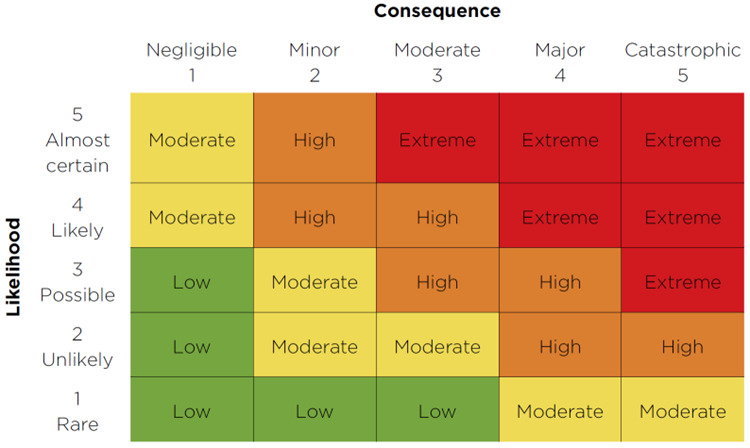
\includegraphics[scale=0.87]{images/riskmatrix.png}
    \caption{Risk matrix of the project, showing a risk-averse appetite}
    \label{fig:riskmatrix}
\end{figure}

\paragraph{Version Control}

Version control is essential in software development to backup and manage the source code of a project and keep track of the history of changes made to the codebase. \textit{Git} was chosen as the version control system to be adopted since it is free, easy-to-use and also provides a cloud-based hosting service for managing repositories known as \textit{GitHub}. Using version control improves efficiency as commits are made after every change, ensuring less time will be used to backtrack the introduction of bugs and errors since the change in each file is clearly recorded and can be reverted back to. 

\paragraph{Risk Action Plan}

Table \ref{tab:riskactionplan} displays several risks associated with the project, their risk level --- measured via the risk matrix in Figure \ref{fig:riskmatrix} --- and their corresponding action plan to remediate the risk.

% \setstretch{1}
\begin{table}[H]
    \centering
    \addtolength{\leftskip} {-2cm}
    \addtolength{\rightskip}{-2cm}
    \begin{tabular}{|L{5.1cm}|L{1.5cm}|L{1.5cm}|L{1.0cm}|L{5.1cm}|}
        \hline
        \normalsize{\textbf{Risk}} & \normalsize{\textbf{Likelihood}} & \normalsize{\textbf{Consequence}} & \normalsize{\textbf{Risk Level}} & \normalsize{\textbf{Action}}
        \\ \hline
        Project data being lost, for example, due to hard drive corruption, misplacement of laptop or accidental deletion. & Unlikely & Catastrophic & High & \textit{GitHub} was used to maintain a remote repository and 2 remote backup locations (external hard drives) were also utilised.
        \\ \hline
        Datasets needed for testing and training models not being available --- some need permission and take a long time to gain access to, especially \textit{AffectNet}. & Possible & Major & High & The decision was made to request these datasets early in term 1 during the research phase of the project so that by term 2, all the datasets needed were available.
        \\ \hline
        Requirements of the project change. & Possible & Minor & Moderate & By employing an agile methodology, we significantly mitigate the impact of such an event as we are much more adaptable to changing requirements.
        \\ \hline
        Project is not completed on time, for example, due to illness. & Possible & Major & High & The project's deadline was made to be week 8 of term 2, to increase the sense of urgency to complete the project. If this cannot be achieved a discussion should be had with the project supervisor to discuss contingency plans.
        \\ \hline
        Lack of user involvement --- If users are not involved in the design and testing of the software, specifically the UI, the final product may not meet their needs. & Rare & Moderate & Low & By adopting an iterative methodology, users will be involved at the end of each sprint. 
        \\ \hline
        Imbalances in datasets used to train models may lead to bias, for example, FER-2013 is heavily biased towards `happiness'. & Likely & Moderate & High & Techniques such as data augmentation could be employed to help address class imbalance by creating additional synthetic data points for the minority class, thereby balancing the number of samples in each class.
        \\ \hline
    \end{tabular}
    \caption{Project's risk action plan}
    \label{tab:riskactionplan}
\end{table}
% \setstretch{1.5}

\subsubsection{Time Management}

As mentioned previously, this project was split into two phases, a research phase and a development phase. In the initial stages of the project, we decomposed the project into smaller, more manageable components and created a Gantt chart to schedule the tasks, establish dependencies between tasks and visualize the project timeline which can be seen in Figure \ref{fig:gantt1} in Appendix \ref{appendix:ganttcharts}.
\np
Unfortunately, this initial project timeline was unrealistically optimistic, especially for term 1, as we did not account for various external factors affecting the project, for example, applying for internships or other modules --- such as the machine learning module --- that needed to be studied before certain aspects of this project could be executed properly. However, despite this optimism, we outlined in the specification that it is highly probable that all research tasks scheduled in term 1 will not be completed and so any uncompleted tasks will be rescheduled into the Christmas holiday period, which was previously slack. This did not hinder the quality of the project as we adopted an agile methodology that can better stomach change and uncertainty. Certain tasks, however, are essential for the development phase of the project; requesting datasets early on is critical because large parts of the application development process are dependent on it. Therefore, this task was given very high priority and was completed on time in term 1.
\np
Figure \ref{fig:gantt2} in Appendix \ref{appendix:ganttcharts} shows the actual executed timeline of the project which displays some tasks that have been rescheduled into the \textit{`Christmas Holidays'} period, shown by a black range bar. Term 2 was less busy than term 1 as there were no dependencies on term 2 modules. Therefore, many of the tasks scheduled for term 2 were not only completed on time, but some tasks were actually finished before their allotted deadline. As mentioned before, all high priority tasks were scheduled to be completed by the end of week 8, which was achieved, allowing more time to be dedicated to improving the UI via user testing.


\clearpage
\section{Design}
\label{design}

In this section, we will explore the overarching design considerations that guide the project. Initially, we will define the key components of the project, what exactly we want to achieve and its rationale. This will be followed by an examination of the two primary approaches under consideration for constructing the application: one that employs all pre-trained models in a python backend and another that performs all computations within the browser. Subsequently, we will scrutinize the current technologies adopted in each approach and justify our selection of technologies. Finally, we will discuss and justify the UI design choices in our application and how we aim to evaluate the design.
%%%  mention "how we aim to evaluate the design." ??
\np
The application we intend to design has multiple components to it that are worth clarifying. We aim to design a web application that accesses the user's webcam and records their emotions through their facial expresions. Our objective is to have a model that can categorize facial expressions into a minimum of six distinct emotion classes, utilizing the taxonomy popularised by \cite{ekman} as well as a supplementary emotion class --- `neutral' --- as it is the state of no discernible emotional expression. Moreover, we aim to retrieve other human attributes from the user's webcam, namely, age and sex. As discussed in Section \ref{ourwork} and stated by NFR.4 in Section \ref{nfrs}, ensuring our application is multimodal is essential; we will be looking not only to access the user's webcam, but their microphone too. This is so that the user's spoken words can be converted to text, via speech-to-text technology, which can then be analysed for its sentiment using sentiment analysis. We will also be looking to implement a feature that can inform users whether their lighting conditions are adequate or not, as stated by FR.11 in Section \ref{frs}. Each of these components can be seen in the activity diagram --- a type of unified modeling language (UML) diagram --- shown in Figure \ref{fig:umlactivity}, which shows the tasks that must be done in parallel as the user interacts with the web application.

\begin{figure}[H]
    \centering
    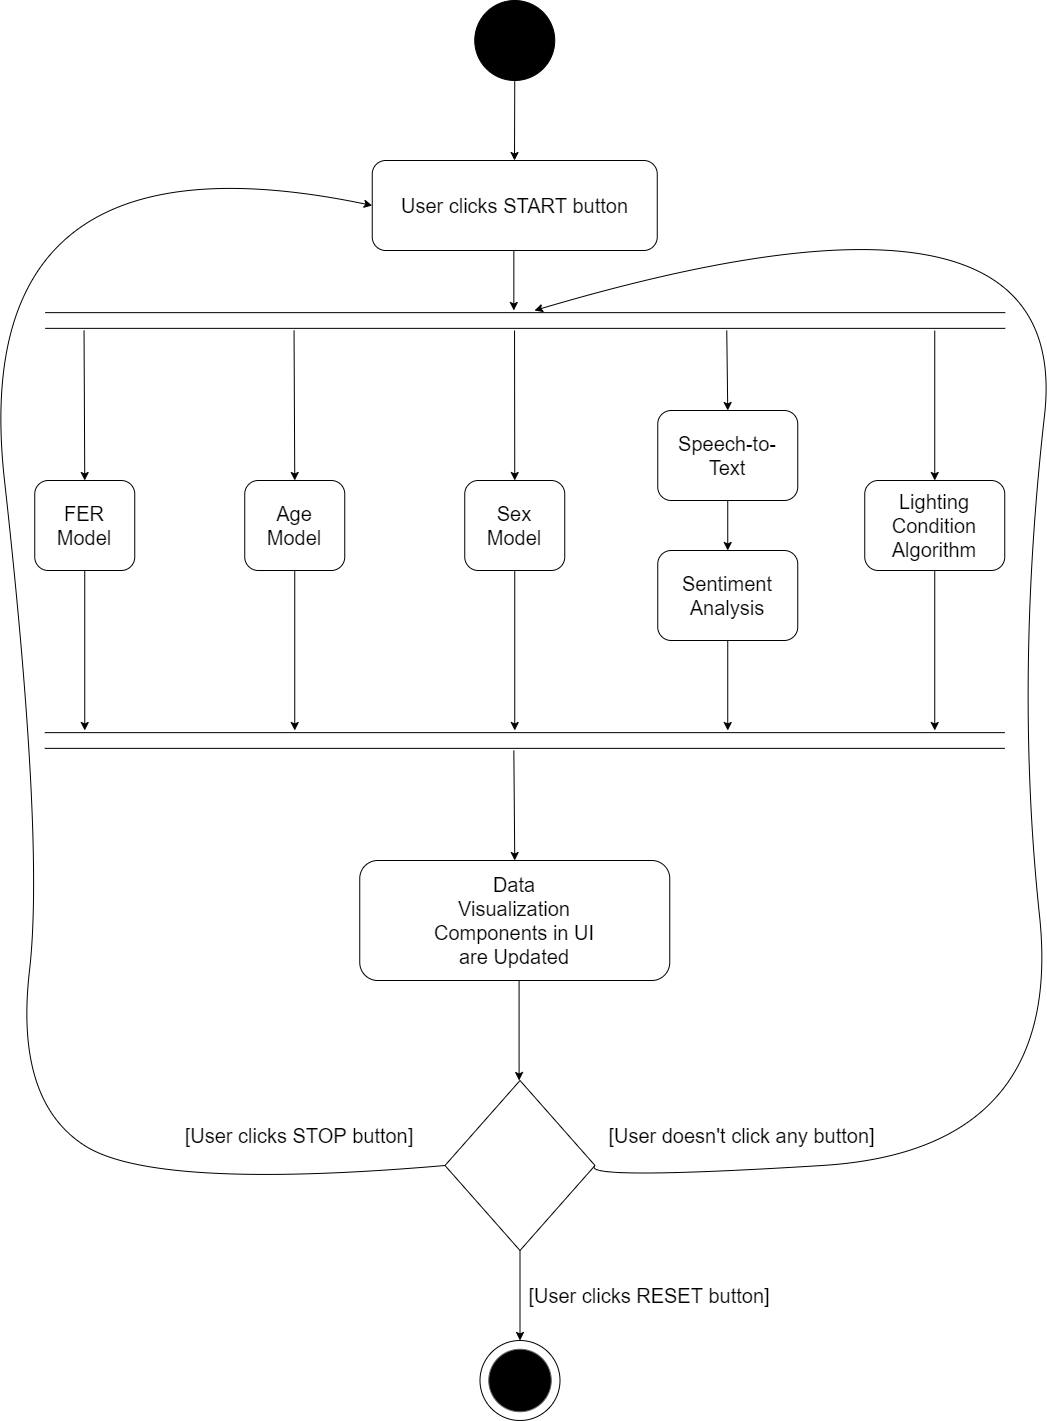
\includegraphics[scale=0.41]{diagrams/activitydiagram.png}
    \caption{UML activity diagram of \textit{RTHAA}}
    \label{fig:umlactivity}
\end{figure}
\clearpage

The data visualization components that we aim to implement, stated by NFR.6, NFR.7 and NFR.8 in Section \ref{frs}, are:

\begin{itemize}
    \item Current emotion status (Figure \ref{fig:uic-bar}) --- Shows the predicted emotion, as well as the predicted percentage chance of other emotions in the form of a bar chart. 
    \begin{figure}[H]
        \centering
        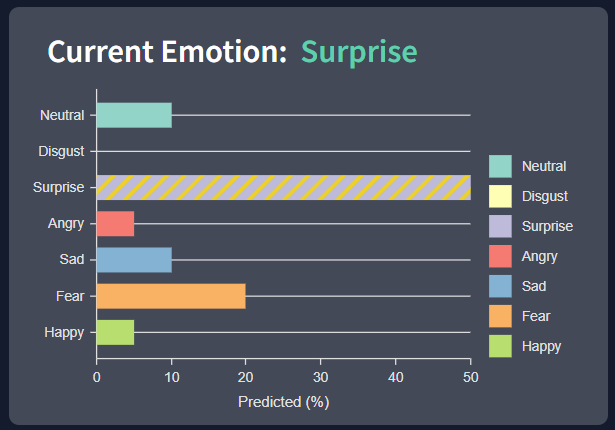
\includegraphics[scale=0.80]{images/uic-bar.png}
        \caption{RTHAA's \textit{`CurrentEmotion'} component}
        \label{fig:uic-bar}
    \end{figure}
    This is a useful data visualization component to have as it shows not only the dominant emotion being displayed, but also the probability of other emotions, providing more useful data.

    \item Emotion-time graph (Figure \ref{fig:uic-graph}) --- Shows how the emotions of a user changed over time.
    \begin{figure}[H]
        \centering
        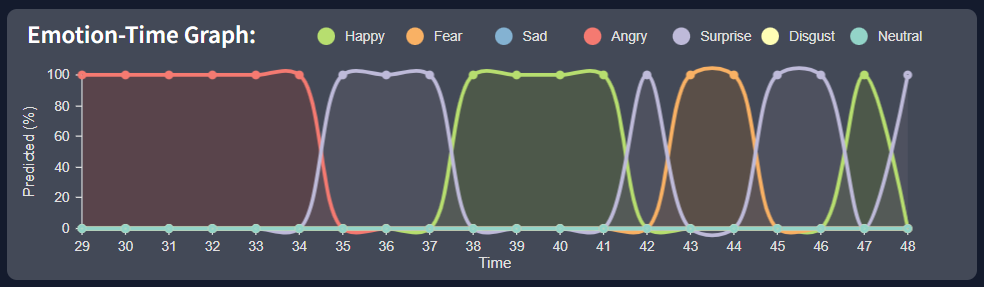
\includegraphics[scale=0.70]{images/uic-graph.png}
        \caption{RTHAA's \textit{`EmotionTime'} component}
        \label{fig:uic-graph}
    \end{figure}

    This is a useful data visualization component as one can see how a user's emotions have changed over time and can therefore map the change in emotions to certain stimuli in whatever environment the user is testing.

    \item Average emotion displayed during test (Figure \ref{fig:uic-pie}) --- Shows the proportion of each emotion the user displayed during the entire test in the form of a pie chart.
    \begin{figure}[H]
        \centering
        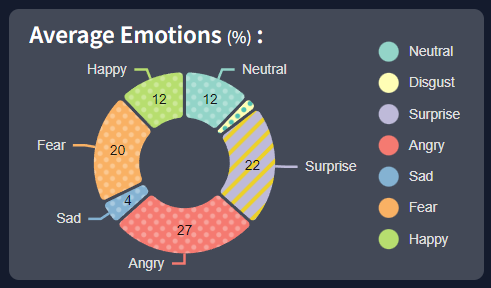
\includegraphics[scale=0.9]{images/uic-pie.png}
        \caption{RTHAA's \textit{`AverageEmotion'} component}
        \label{fig:uic-pie}
    \end{figure}

    This is a useful data visualization component as one can quickly determine the user's overall experience of a system, for example, if the pie chart contains 75\% happy and 25\% neutral, we can deduce that the user had a positive overall experience using the system.

\end{itemize}

\subsection{System Architecture}
\label{sysarch}


%% Do frontend processing, and backend processing architecture


% Discuss the two approaches, then the technologies, then include a diagram

When developing the web application, two primary system architectures were evaluated. The first architecture involves utilizing the webcam located on the frontend of the application, which captures individual frames at a specified frequency, along with the transcript of the user's speech --- which has been retrieved by converting the user's speech to text --- and sends them to a backend. In this design, the frames are processed by pre-trained models located in the backend, which classify the emotion, age and sex predicted in the received frame, as well as the sentiment of the user's speech. The output generated by the pre-trained models is then transmitted back to the frontend, where it is presented to the user. Alternatively, the second system architecture under consideration was simpler and involved processing all the data within the frontend, without the use of a backend server.
\np
%%% OPPORTUNITY TO CONDENSE
Each architecture has its own set of advantages and disadvantages. Using a backend means that the processing load is offloaded to a backend server, which can handle more complex computations more efficiently. This means users with weaker devices, such as older generation phones, can still use the application the same way someone on a powerful laptop would be able to, as the bulk of the processing is done remotely. Furthermore, having the computation on the backend separate from the frontend, means that the backend can be easily updated and improved without affecting the frontend code, however, due to the software architectural pattern we employ, which will be discussed in Section \ref{sap}, the data logic will be abstracted away from the UI code anyway, regardless of the system architecture used. However, using a backend poses some disadvantages too. Firstly, the application relies heavily on internet connectivity, as it is constantly sending images across a network which is expensive and slow, causing there to be a delay between the capture of the frames and the output displayed, making the application less real-time. 
\np
In addition, there are privacy implications that need to be considered as users may feel uneasy about sending their personal information, such as their age and sex, to a remote server where it could potentially be stored and misused if adequate safeguarding procedures are not implemented. The second architecture proposed where all data processing is done in the frontend, has the advantage of being simpler to develop and maintain, as it does not require a backend server. Moreover, this approach can offer faster performance as there is no delay caused by transmitting images to a backend and waiting for a response. Additionally, the application can operate without a constant internet connection after the initial page is retrieved, as all processing can be performed locally, which also nullifies any potential privacy issues. Figures \ref{fig:febe} and \ref{fig:allfe} in Appendix \ref{appendix:sad} show the high-level design of the two system architectures under consideration. Their technologies are justified in Section \ref{tfl}.
\np
The decision was made to implement an architecture that utilises a remote server, to provide users with the convenience of remote processing. However, in hindsight, it was realized that this decision may not have been the best course of action. Despite the processing being done remotely, the user is still required to transmit a stream of images for an extended period of time, which puts significant computational stress on the user's device, more so than what the pre-trained models working locally would have. This will be discussed more in Section \ref{implementation}, where we compare the performance of the implementations of both architectures. Despite implementing the architecture that uses a remote server, we still had time to implement the frontend-processing architecture as we were more familiar with the tools and technologies involved in the process and we had chosen a more development-oriented methodology.

\subsection{Tools, Frameworks and Libraries}
\label{tfl}

In this section, we justify the selection of the languages, frameworks and libraries employed in the development process of both architectures. As we are looking to develop an interactive, dynamic web application, as opposed to a static web page, JavaScript must inevitably be used. Dynamic web applications have interactive and real-time user interfaces. JavaScript adds dynamic functionality to web pages, such as live data visualizations, without requiring a full page reload. 

\subsubsection{Selecting a JavaScript Framework}

Building complex dynamic pages using raw JavaScript can be tedious as it has no standard library and has confusing syntax as there are multiple ways of defining semantics \citep{jsbad}. Consequently, JavaScript frameworks that aim to ease and speed up the development process have grown substantially in popularity \citep{delcev2018modern}. As the JavaScript framework determines what the user sees and how they interact with the web application, selecting an appropriate framework is pivotal. As stated by \cite{saks2019javascript}, the current, most popular JavaScript frameworks in web development are React.js, AngularJS and Vue.js.
\np
Of the three aforementioned JavaScript frameworks, React.js was ultimately chosen for many reasons:

\begin{itemize}
    \item React.js is more suitable for single-page applications compared to AngularJS and Vue.js as its syntax centres around the idea of reusable components \citep{arv} --- chunks of UI that constitute the single page application that can be used any number of times --- which simplifies development and makes the code easier to manage and maintain.
    
    \item React.js has a larger community and ecosystem with a wealth of third-party libraries, more so than AngularJS and Vue.js \citep{arv}. This reduces development overhead because it allows for us to take advantage of reuse-oriented software development as mentioned in Section \ref{sdm}. Consequently, we can use libraries like Material UI and Nivo which significantly cut down on writing unnecessary code by offering reusable UI components. 
    
    \item Since our application has a lot of dynamic content, such as live graphs and pie charts, the page will be re-rendering very frequently. React.js is known for its excellent performance, particularly in terms of rendering speed. This is mostly due to React.js having the most efficient virtual document object model (DOM) implementation, compared to AngularJS and Vue.js \citep{vdom}. The DOM is a programming interface for web documents which represents a document as a tree structure, shown in Figure \ref{fig:dom}, where each node in the tree corresponds to a document object. The virtual DOM refers to a lightweight, in-memory representation of the actual DOM tree that is used to optimise the process of updating the UI by updating only the parts of the actual DOM tree that need to change, hence resulting in faster rendering.

    \begin{figure}[H]
        \centering
        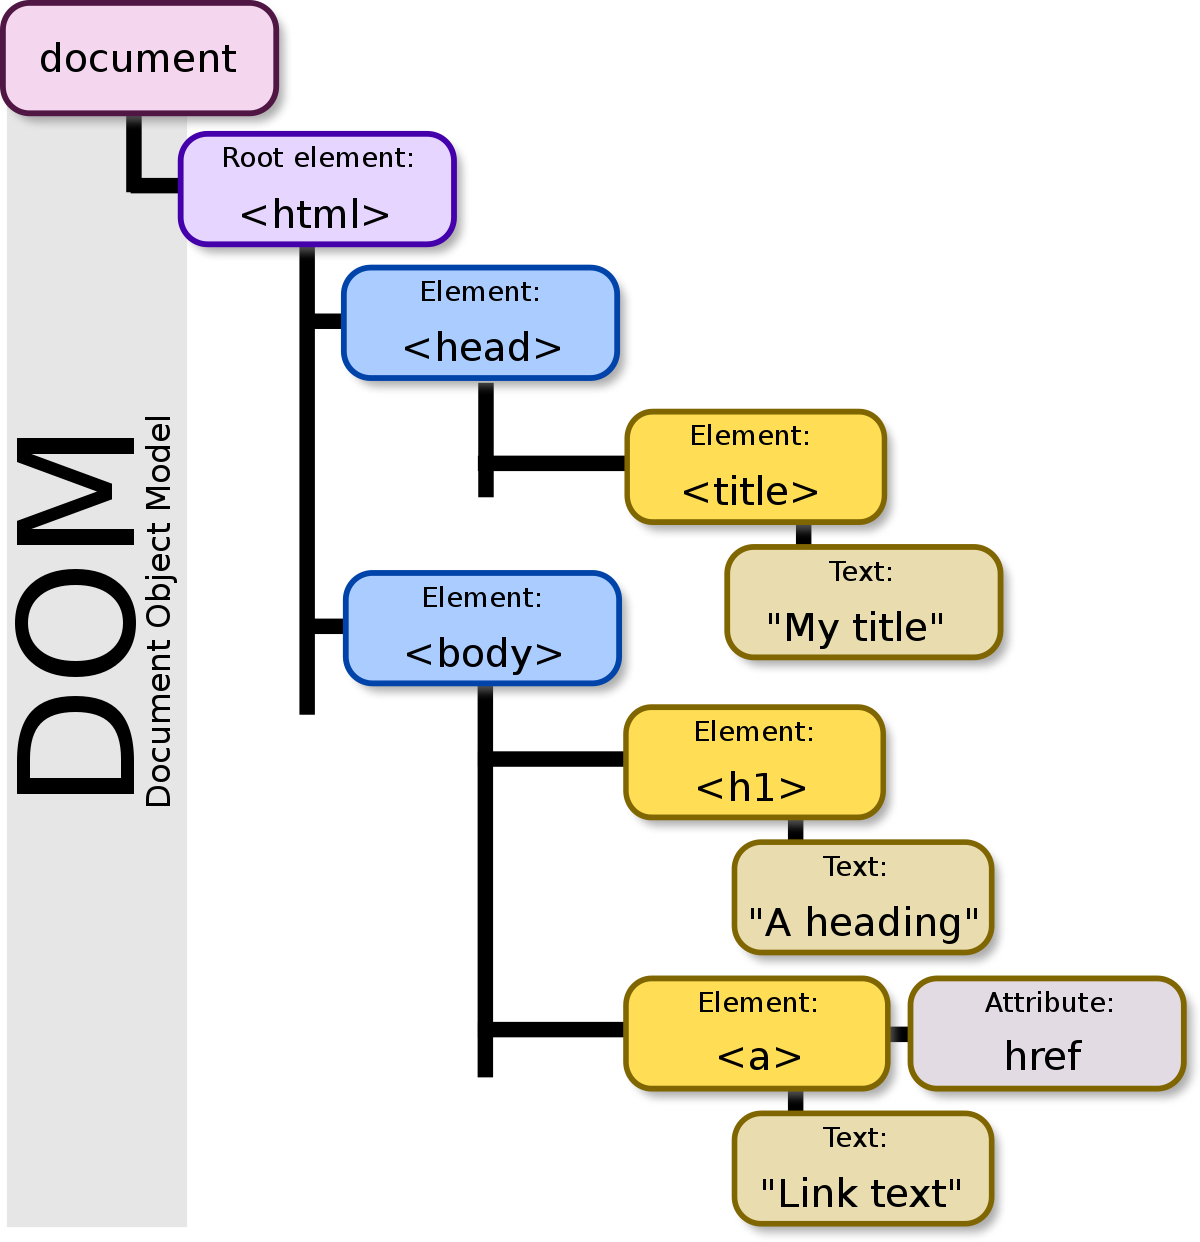
\includegraphics[scale=0.3]{images/dom.png}
        \caption{Visual representation of the DOM, taken from \cite{wikidom}}
        \label{fig:dom}
    \end{figure}

    %% Add back?
    % \item React.js is syntactically structured in a way that lends itself easily to the software architectural pattern we look to employ --- model-view-controller (MVC) --- which will be discussed in more depth in Section \ref{sap}. This can make code easier to read and understand as well as help reduce the risk of errors. However, it is worth noting that AngularJS, like React.js, employs the MVC architectural pattern, as stated by \cite{arv}.
    
\end{itemize}

\subsubsection{Other Technologies Used}
\label{othertech}
Apart from React.js, other technologies were also utilized. These include Python and Flask, for use on the backend of the application. TensorFlow, Keras and matplotlip will also be used to help evaluate the performance of pre-trained models, as well as for conducting EDAs on various datasets. The justification of each tool is as follows:

\begin{itemize}

    \item \textbf{Python} --- Python has an extensive range of libraries, including NumPy, Pandas, Matplotlib, Scikit-learn and TensorFlow, that can help to simplify complex operations in machine learning and hence will be used when assessing pre-trained models to be used for the web application.

    \item \textbf{Flask} --- Flask is a lightweight web framework used to build full-stack web applications that have Python on the backend. Another popular Python web framework is Django, however, this was not chosen due to it being more for database-driven applications \citep{flaskdjango}.

    \item \textbf{TensorFlow \& Keras} --- TensorFlow is an open-source library for creating and training machine learning models. Keras is an open-source deep learning framework built on top of TensorFlow and provides a high-level application programming interface (API) for building deep neural networks. PyTorch was also considered as an alternative machine learning framework to TensorFlow, but was not chosen because of its smaller community and ecosystem \citep{tfvspytorch}.

    \item \textbf{Matplotlib} --- Matplotlib is a data visualization library for creating plots, graphs, charts, histograms and other types of visualizations from data in Python. It will mainly be used in the process of evaluating the performance of pre-trained models as well as for conducting EDAs on datasets.
    
    \item \textbf{Nivo} --- Nivo is a React.js library that provides a rich set of data visualization components and will be used for displaying the graphs, pie charts and bar charts in our application.
    
    \item \textbf{Material UI} --- Material UI is a React.js library that offers a comprehensive suite of tools that help develop UIs faster.

\end{itemize}

\subsection{UI Design}
\label{uidesign}

Designing a good user interface is essential because it directly affects how users interact and experience the application. A well-designed UI can make a great first impression on the user, starting their user experience with a positive tone. A primary consideration in the design of user interfaces in web applications is accessibility for users with disabilities, such as visual or hearing impairments. We will be looking to follow accessibility guidelines and standards, such as the WCAG, discussed in Section \ref{adduid}, to ensure that the interface is inclusive and can be used by all users.
%%% Are you sure you want to mention WCAG??
\np
Initial drafts and high-level design considerations of the UI were developed by considering the content of the application, for example, having a symmetrical layout. The window showing the user's webcam was centred on the page, as this creates a more balanced and visually appealing aesthetic. Furthermore, when the webcam window is in the centre of the page, the user can look at their own face while staring straight ahead. If the webcam window was on the side of the page, the user would have to look to the side to see themselves, and in the webcam footage, they would be looking to the side instead of straight ahead. The webcam footage was also made to be horizontally inverted as it can be quite distracting when a user, for example, moves their head right, but in the webcam window, their head turns left. The combination of these two design ideas leads to the user's movements being more intuitively represented on screen. Figure \ref{fig:uidraft} shows the very first draft created for the design of the UI. Figure \ref{fig:webappHss} shows the centred webcam window, with all the data visualization components surrounding it in the final design of RTHAA. 

\begin{figure}[H]
    \centering
    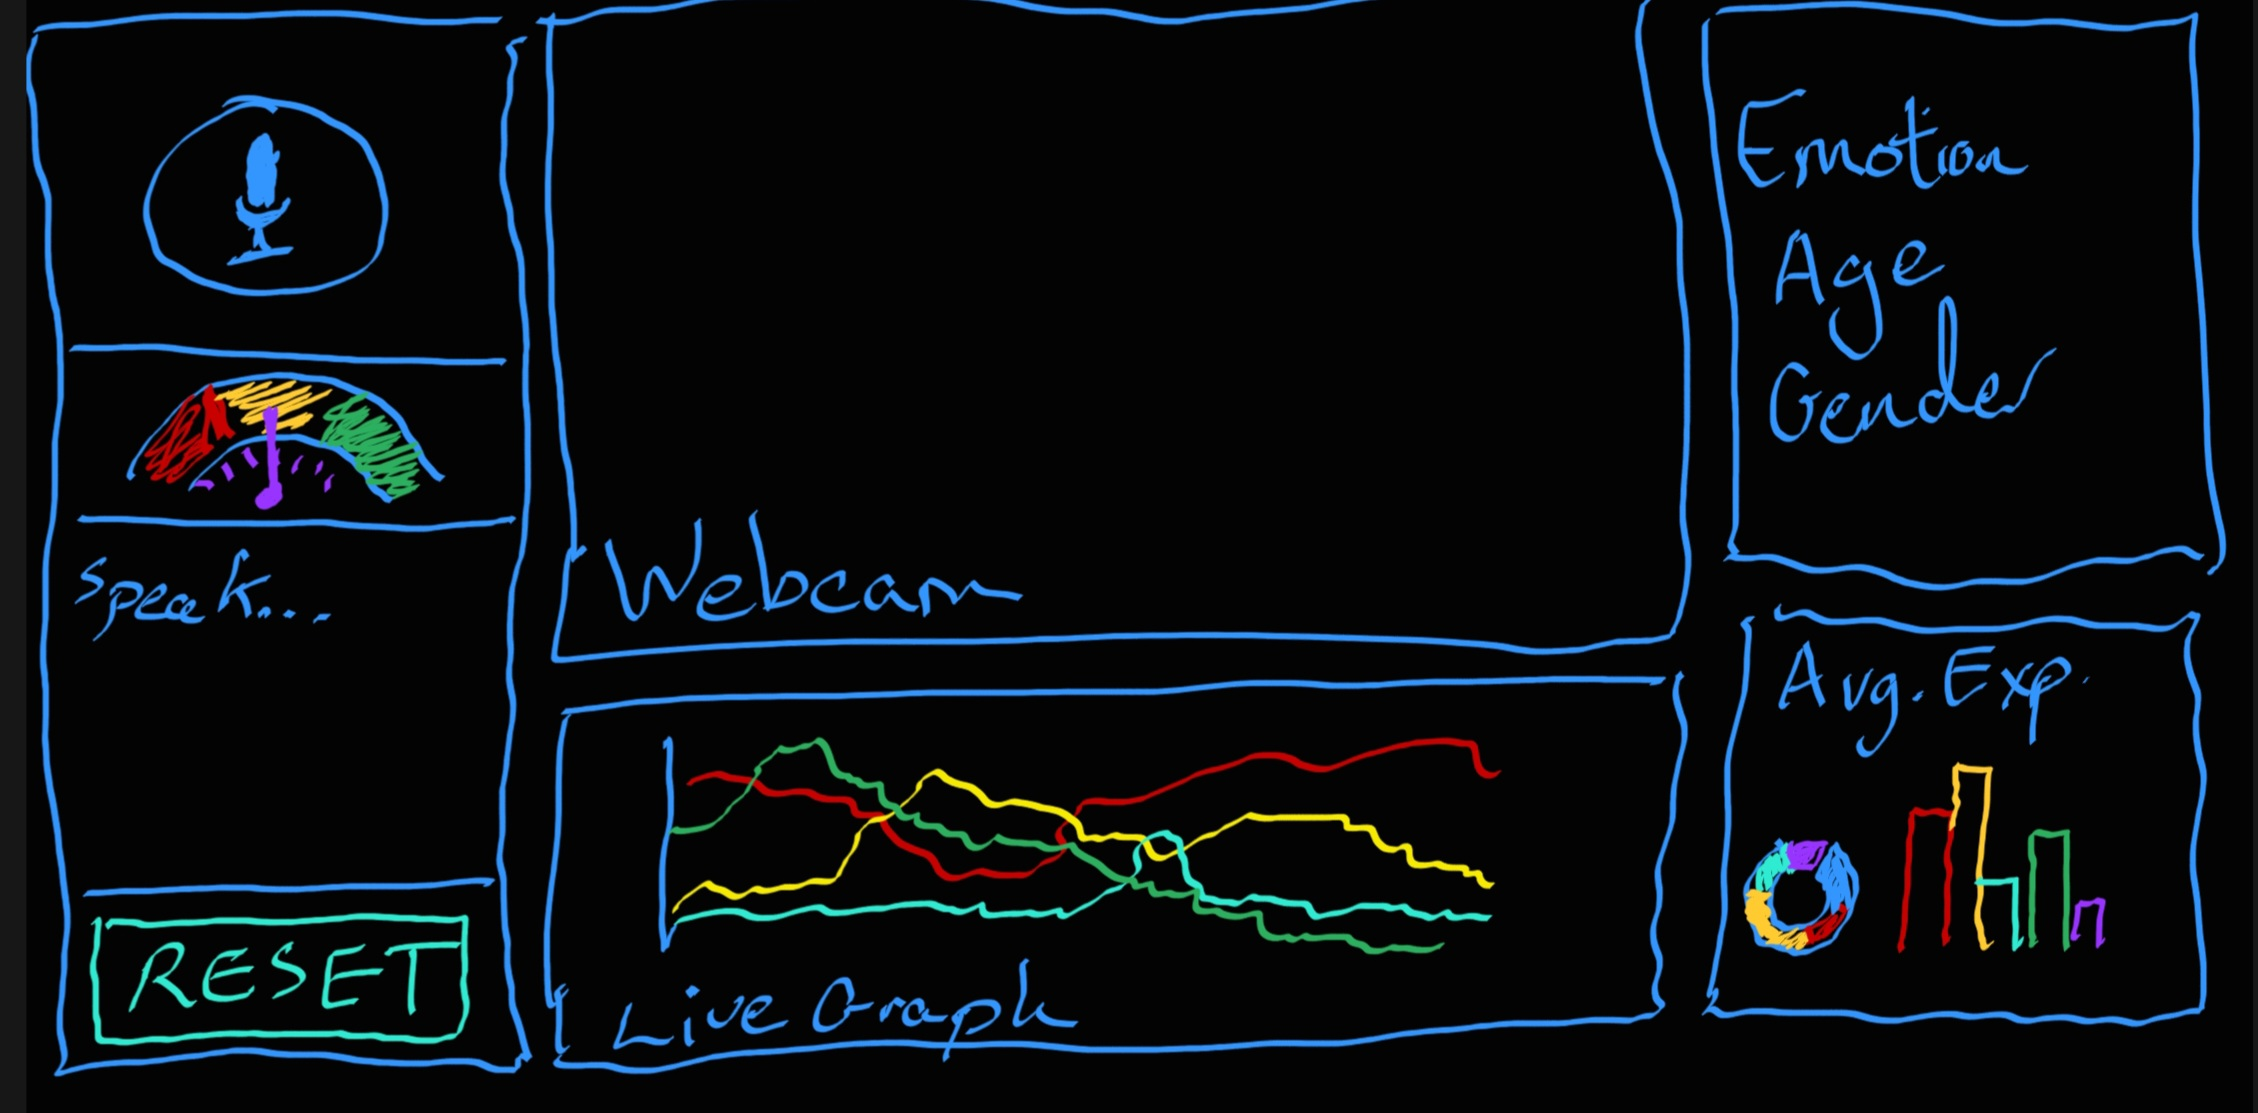
\includegraphics[scale=0.18]{images/uidraft.jpg}
    \caption{Very first draft of UI design}
    \label{fig:uidraft}
\end{figure}

\begin{figure}[H]
    \centering
    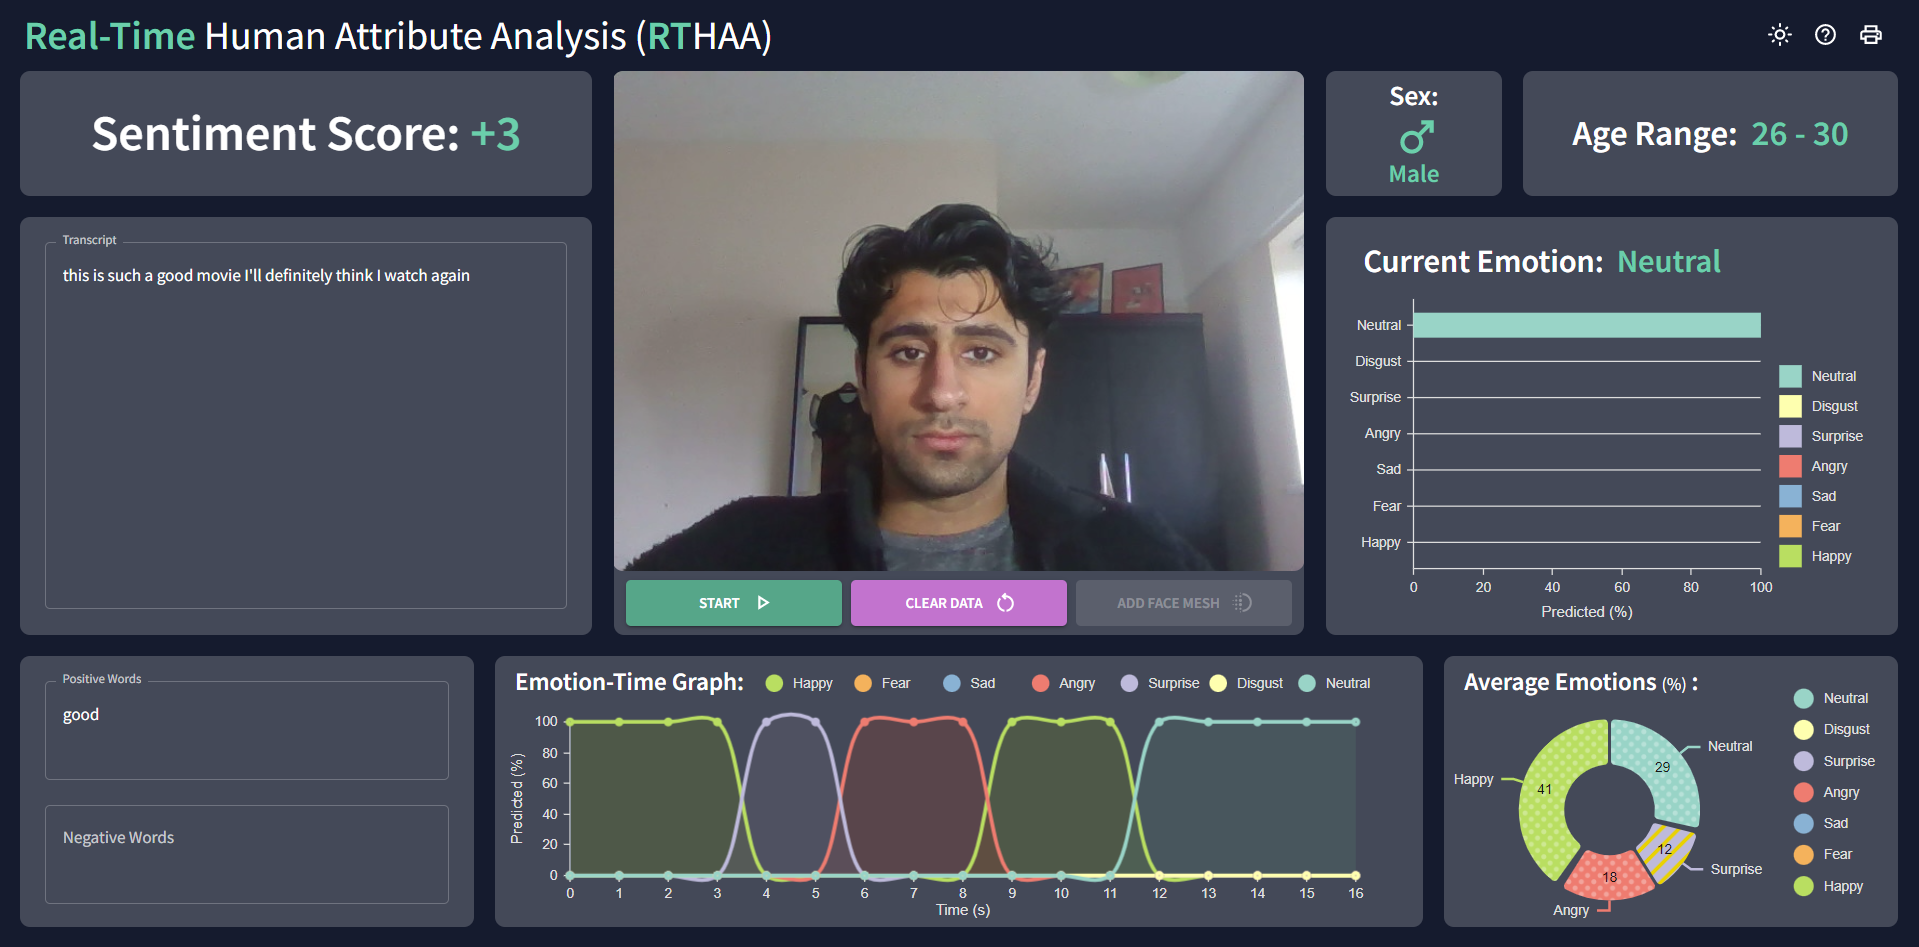
\includegraphics[scale=0.36]{images/webappFE13H.png}
    \caption{Screenshot of the UI of the finished application}
    \label{fig:webappHss}
\end{figure}

As shown by Figures \ref{fig:uidraft} and \ref{fig:webappHss}, the UI design hasn't changed significantly since its initial inception, due to care being taken by ensuring that common UI design practices were being followed. However, the design has still undergone some change as a result of user feedback at the end of each development sprint. The primary aim of the design was for it to be clean, simple and intuitive. All the data visualization components were made to be put on a single dashboard for the purpose of navigation, so that it becomes very easy for users to obtain the information they require. However, one concern was that the UI may become too clogged. To combat this, a minimal UI design was created, with a non-intrusive colour scheme. The colour scheme employs a dark blue color for the background and uses lighter, grayish hues for the boxes that contain text and data visualization elements. Additionally, white and a deep-sea green colour is used for text. The use of dark colors for the backdrop and white text creates a high contrast, increasing accessibility and contributing to a sleek and minimal design that conveys a sense of professionalism. 
\np
Two central design principles were adopted to guide the UI design process, namely, the Gestalt laws of perceptual organisation \citep{todorovic2008gestalt} and Nielsen's usability principles \citep{nielsen1994usability}. The Gestalt principles were employed as they are the widely-accepted general theory of perception in psychology, as stated by \cite{mather2006foundations}. The principles are not just restricted to interfacing with a computer, but how we as human beings process visual information more generally. Nielsen's usability principles were also adopted in the design process as they are regarded as the standard methodology for user interface design in web development \citep{uineilson}. More detail as to how these principles were implemented will be discussed in Section \ref{uii}.

\clearpage

\section{Implementation}
\label{implementation}

Developing a real-time web application that is capable of detecting emotion, speech sentiment, age, sex and lighting conditions involves piecing together many different components. In this section, we will first discuss the implementation of the architecture which uses a remote server, focusing on the backend, and why it was not chosen as the final system architecture. We will then give a high-level overview of how the frontend-processing architectutre was implemented.

\subsection{Remote Server Architecture Implementation}

In this section we discuss how the first architecture proposed in Section \ref{sysarch}, which utilises a remote server, was implemented. It is worth nothing that the frontend for this architecture, primarily consisting of the UI, was not fully implemented, since once the main functionality of the application was deemed too slow, there was no point in developing the UI for it. This decision allowed more time for the development of the more performant, frontend-processing architecture.
\np
As mentioned in Section \ref{othertech}, Flask was the python web framework used on the backend. The flow of the data would be as follows: the frontend retrieves individual frames from the user's webcam, as well as the transcript of their speech, and sends it to the Flask backend for it to be processed. The backend would then emit the outputs of the models back to the frontend for it to be displayed. 
\subsubsection{WebSockets}

In order to speed up the transmission between the backend and frontend, WebSockets were used instead of traditional HTTP requests. A socket is one endpoint of a two-way communication link between two programs on the network. WebSockets are a type of communication protocol that allow for real-time, bidirectional communication between a client and a server over a single, long-lasting connection, through the interface of a socket. They allow for real-time data exchange without the need for continuous HTTP requests, reducing network overhead and conserving bandwidth. As the communication is full-duplex, i.e. bidirectional, both the client and server can send data to each other simultaneously. In summary, WebSockets were employed as they provide a much faster and more efficient way of exchanging data compared to HTTP requests, which can help reduce latency and improve overall performance in real-time applications. Figure \ref{fig:codews} shows a code snippet of how the communication between the backend and frontend was established in Flask using the \verb+Flask-SocketIO+ library which implements the WebSocket protocol.

\begin{figure}[H]
    \centering
    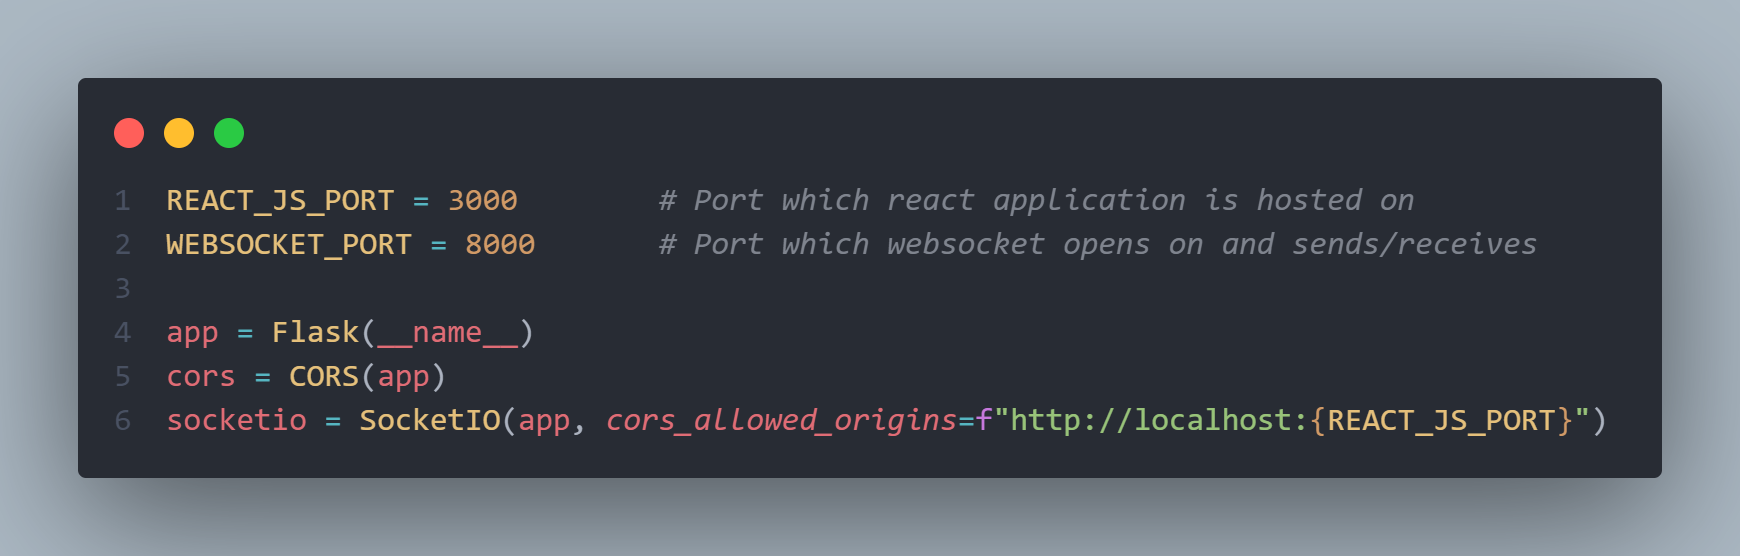
\includegraphics[scale=0.23]{images/codews.png}
    \caption{Code snippet of how Flask's implementation of WebSockets were used to establish the connection between the backend and frontend}
    \label{fig:codews}
\end{figure}

In line 6 of Figure \ref{fig:codews}, you can see the keyword arguement \verb+cors_allowed_origins+ being used. Cross-Origin Resource Sharing (CORS) is simply a security mechanism that allows a web page to request and access resources from a different domain than to the one the page itself came from, a feature which is blocked by default on most browsers. In our case, CORS needs to be used because the page itself is being hosted on a server with port 3000, as shown by \verb+REACT_JS_PORT+ in line 1 of Figure \ref{fig:codews}. However, the page attempts to access a different port on a different server, specifically port 8000, as shown by \verb+WEBSOCKET_PORT+ in line 2 of Figure \ref{fig:codews}, which is the server that actually processes the data. By using CORS, our web application can override the browser's default settings and can securely access multiple servers.
\np
An example of how the backend interfaces with the frontend is seen in Figure \ref{fig:codewssa}, which shows how the backend server receives the transcript of the users speech, conducts sentiment analysis on it, and emits the results back to the frontend. The server listens on the socket \verb+"text"+ and once it receives the transcript from the frontend, which will be stored in the function arguement \verb+text+, it conducts sentiment analysis on \verb+text+ using the \verb+TextBlob+ library, a simple NLP library. Once the sentiment data of the text has been computed, a dictionary containing the sentiment data is emitted back to the frontend to be displayed to the user.

\begin{figure}[H]
    \centering
    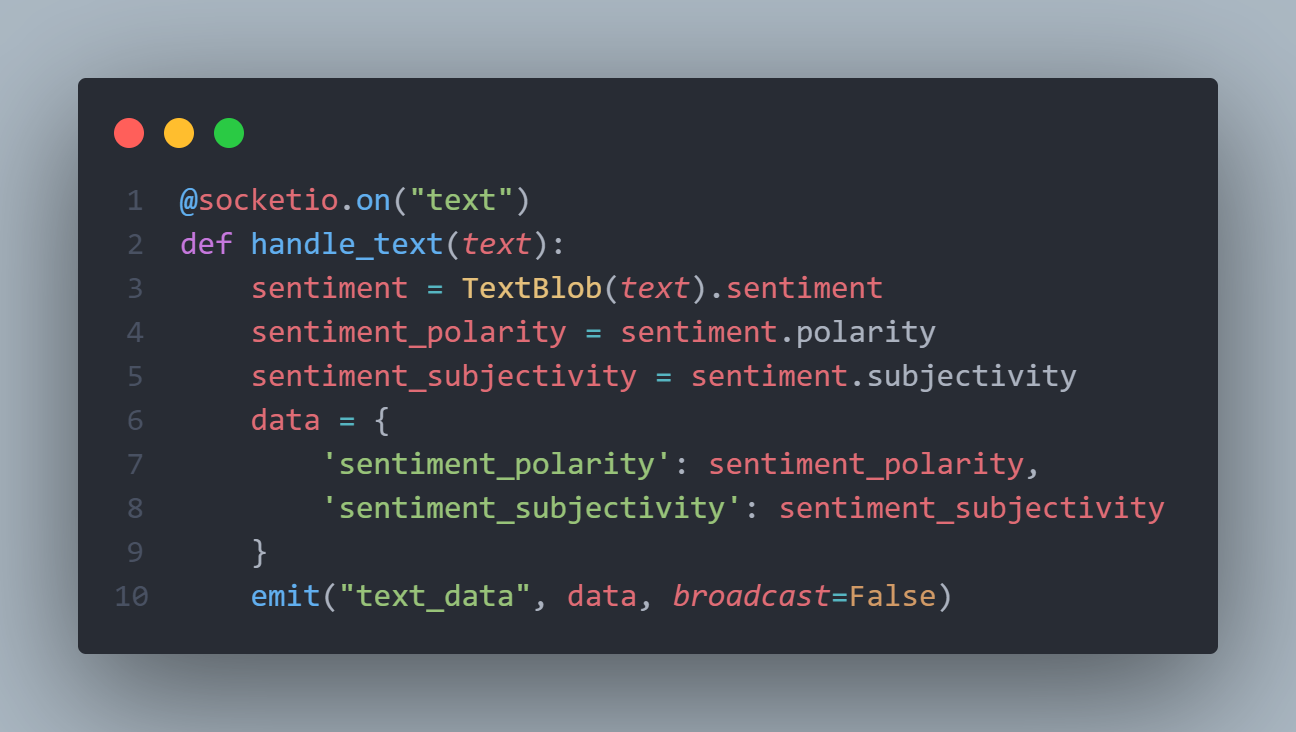
\includegraphics[scale=0.3]{images/codewssa.png}
    \caption{Code snippet showing sentiment analysis of the user's speech on the backend}
    \label{fig:codewssa}
\end{figure}

Ultimately, however, the system architecture which uses this remote backend was not used in the end as it was deemed to slow, violating the non-functional requirement, NFR.8, stated in Section \ref{nfrs}. Table \ref{tab:bevsffe} shows the response times of the backend-processing architecture compared to the frontend-processing architecture when processing the frames retrieved from the users webcam at a frequency of 1 frame per second.

\begin{table}[H]
    \centering
    % \addtolength{\leftskip} {-2cm}
    % \addtolength{\rightskip}{-2cm}
    \begin{tabular}{|L{2cm}|C{5cm}|C{5cm}|}
        \hline
        \normalsize{\textbf{Frame of webcam}} & \normalsize{\textbf{Remote Server Average Response Time (seconds)}} & \normalsize{\textbf{Frontend-processing Average Response Time (seconds)}}
        \\ \hline
        Frame 1 & 3.29 & 0.23
        \\ \hline
        Frame 2 & 3.97 & 0.43
        \\ \hline
        Frame 3 & 5.61 & 0.18
        \\ \hline
        Frame 4 & 9.86 & 0.21
        \\ \hline
        Frame 5 & 17.43 & 0.37
        \\ \hline
    \end{tabular}
    \caption{Comparison of response times between the two architectures proposed when processing the frames retrieved from the user's webcam at a frequency of 1 frame per second}
    \label{tab:bevsffe}
\end{table}

The results in Table \ref{tab:bevsffe} were obtained by conducting a test which defined a function that would wait in intervals of 1 second, sample a frame from the webcam to send to the backend, and wait until the response was retrieved, recording the time period from when the frame was sent. Evidently, the results indicate that the performance of using a backend is too slow for our real-time purposes, and in fact becomes increasingly worse, simply because it can be easily overwhelmed and hence would not be a scalable architecture. This motivated the architecture where all the processing of data is done entirely in the frontend, i.e. the frontend-processing architecture, removing the latency and computational burden of image transmission. In Section \ref{implementation}, we will focus on discussing the frontend-processing architecture, which was the final architecture used. While the implementation of the backend architecture is available in the submitted ZIP file, it will not be further discussed as it was not the architecture ultimately employed.

\subsection{Final Implementation}
\label{finalimp}

In this section, we will discuss the final implementation of \textit{RTHAA}, which uses the frontend-processing architecture. We will begin by explaining some basic concepts in \textit{React.js}, as it forms important background knowledge for understanding the basics of the software involved.
\begin{itemize}

    \item \textbf{Components} --- In React.js, a \textit{component} is a reusable piece of UI that can be used to build complex UIs. A component is typically a JavaScript function that returns a piece of UI in the form of JSX, which is a syntax extension for JavaScript that allows you to write HTML-like syntax. It is possible to nest components and use \textit{props} to enable communication between a component and its subcomponents.
    
    \item \textbf{Props} --- \textit{Props} are a mechanism to pass data from a parent component to a child component. Props are read-only objects that contain data needed by the child component in order to render.
    
    \item \textbf{State} --- In React.js, \textit{state} is a feature that allows a component to store and manage its own internal data. It represents the current condition of a component, which can be changed. One can think of state as a live variable whose value determines what is dynamically rendered by a component that is dependent on said variable. 

\end{itemize}

\subsubsection{Software Architectural Pattern}
\label{sap}

In this section, we will explore and justify the software architectural pattern employed in the development of \textit{RTHAA}, as it provides a high-level overview of the application's organisation and functionality by breaking \textit{RTHAA} down into its components.
\np
The software architectural pattern adopted for organising the codebase of \textit{RTHAA}, was the model-view-controller (MVC) pattern. MVC separates the user interface (the view) part of the code from the data processing (the controller)  part, meaning the UI can be easily changed without affecting the data logic, or the data itself(the model). This  provides a nice abstraction that separates implementation components, helping to reduce code complexity and bugs. Furthermore, the separation of the model, view and controller makes it easier to write tests for each component as the interface to each component is very clear. Consequently, modification to the application is made easier. Since the requirements of the project were unstable at the start, ensuring modification is as easy as possible, would be very beneficial as it allows us to better stomach changes in requirements, compared to other, more rigid, architectural patterns, such as \textit{pipe and filter}, which are more monolithic in structure.
\np
Figure \ref{fig:mvc} in Appendix \ref{appendix:sad} shows how MVC was implemented in \textit{RTHAA}. The user interface, the view, is rendered by the \verb+<Dashboard>+ component, inside of which are multiple subcomponents corresponding to the data visualization components in the screenshot of the final UI, shown in Figure \ref{fig:wa9} in Appendix \ref{appendix:ass}. When the user clicks the start button, the application begins loading the models. This is achieved via the use of state variables, the most important of which are shown in Figure \ref{fig:codestatevars}. When the user clicks start, the \verb+processing+ state variable is toggled, causing a function dependent on \verb+processing+ to load the models as shown in Figure \ref{fig:mvc} in Appendix \ref{appendix:sad}. This forms the controller part of the application. After the controller loads the models that process the webcam footage, the output of the models, i.e. the emotions of the user, their sex, etc. are stored in state variables. These state variables are passed down as props through to the corresponding components. As these state variables change, the components immediately re-render, displaying new data.

\begin{figure}[H]
    \centering
    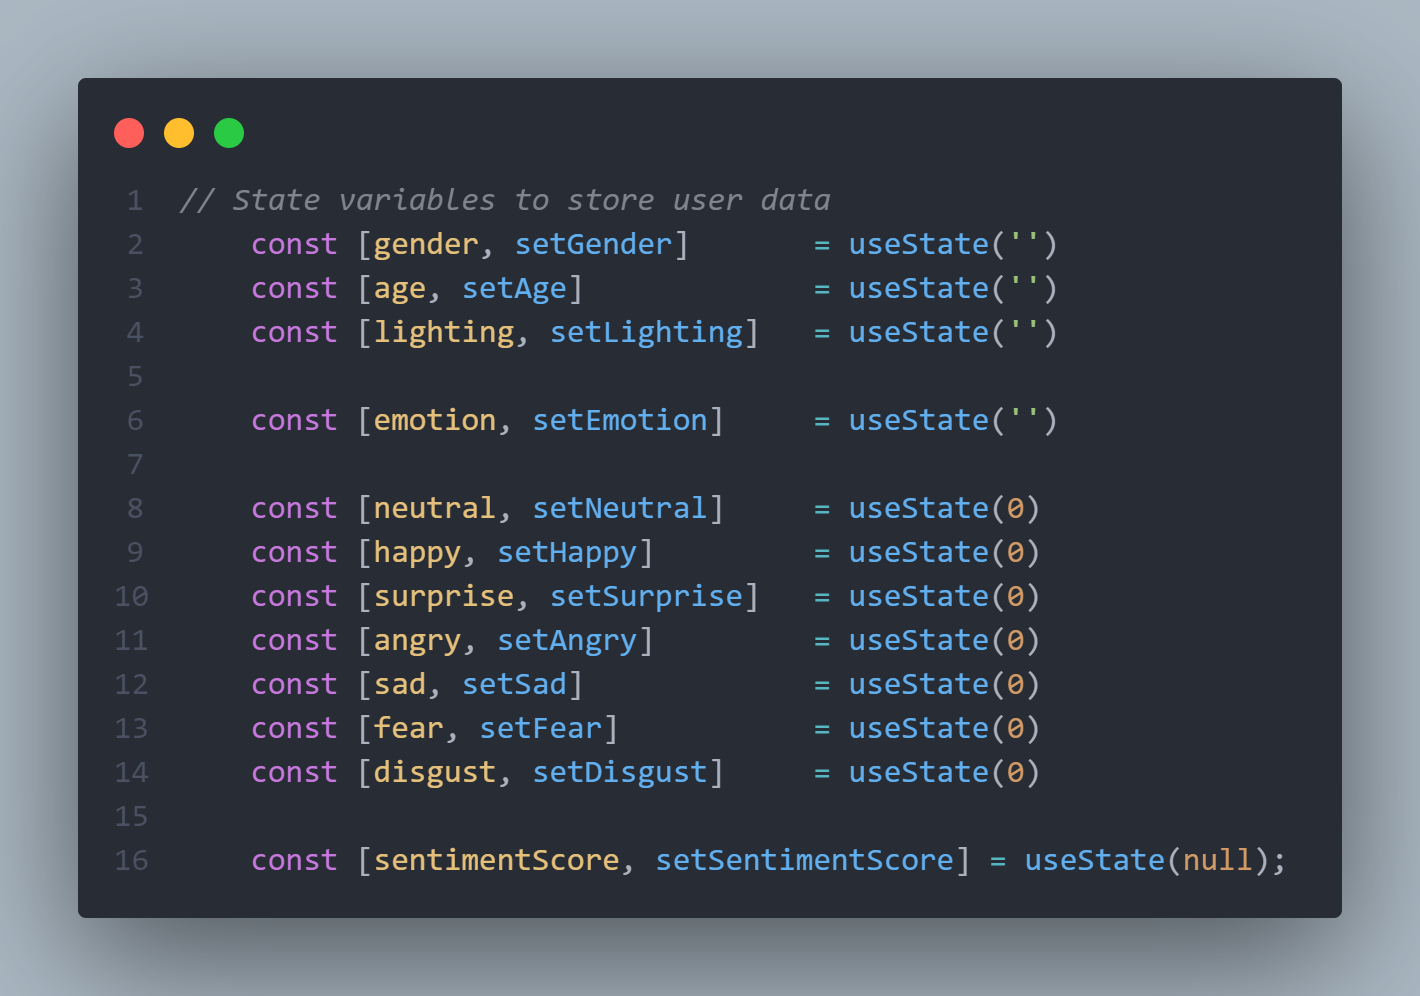
\includegraphics[scale=0.29]{images/codestatevars.png}
    \caption{Main state variables storing user data}
    \label{fig:codestatevars}
\end{figure}

\subsubsection{Speech Recognition}
\label{srecog}
Speech recognition is a technology that enables a computer to recognise and transcribe spoken words into text. Here we describe how the user's speech was converted to text, so that a transcript of the user's speech could be obtained, allowing us to conduct sentiment analysis on it.
\np
In order to convert the user's speech into text, React.js's \verb+react-speech-recognition+ library was used. It provides state variables that give us access to a transcript of speech picked up from the user's microphone. Under the hood, it uses Web Speech API, an API which enables us to incorporate voice data into our application. This library was chosen as the speech recognition library as it is widely used by many commonly used applications such as \textit{Duolingo}, \textit{Google Translate}, and for voice search in \textit{Google} \citep{webspeechapi}. 

\subsubsection{Sentiment Analysis}
\label{sentanal}

In this section, we discuss the implementation of how sentiment analysis was conducted on the transcript of the user's speech. The transcript is stored in a state variable, which is updated every time a new word is recognised from the speech recognition library discussed in Section \ref{srecog}. Consequently, this allows us to dynamically conduct sentiment analysis on the user's speech, as the transcript is updated with new words. This was achieved via a \verb+useEffect+ hook that was listening on the state variable containing the transcript. A \verb+useEffect+ hook allows us to run a specificed function when the state of a state variable changes. In this case, the function conducts sentiment analysis on the transcript state variable. Figure \ref{fig:codesa} shows the arguements of the \verb+useEffect+ hook, the first being the function to execute once the variable the hook is listening to changes, and the second being the list of state variables the hook listens to, in this case, just the \verb+transcript+ state variable.
\np
\begin{figure}[H]
    \centering
    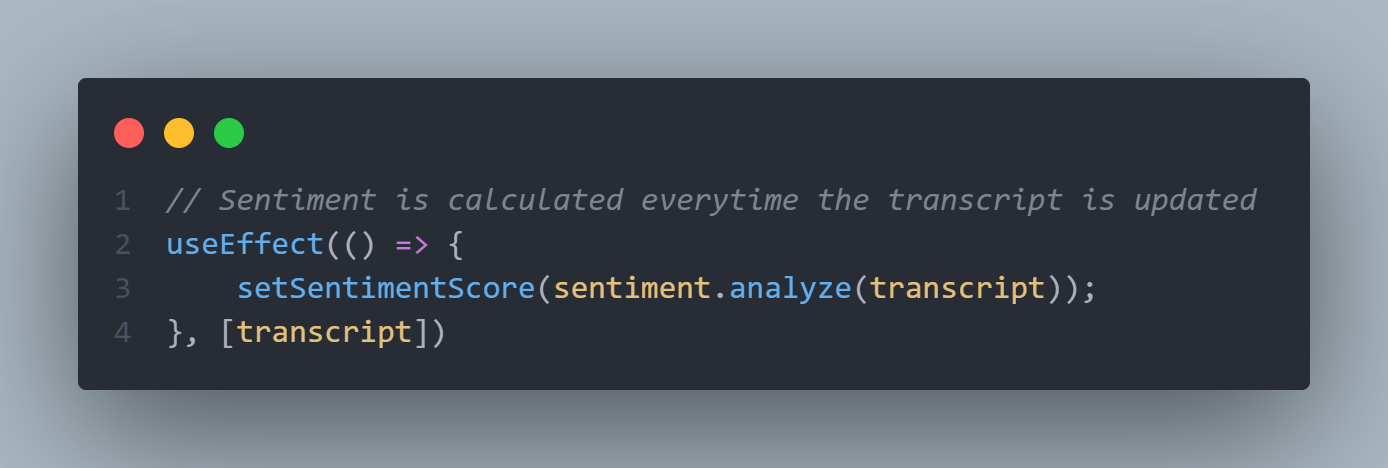
\includegraphics[scale=0.28]{images/codesa.png}
    \caption{Code snippet showing how a \textit{useEffect} hook is used to conduct sentiment analysis on the transcript everytime it is updated by verbal input}
    \label{fig:codesa}
\end{figure}

\paragraph{Selecting an Appropriate Model}
\label{saam}

Given that the transcript is updated every time a single word is spoken, conducting sentiment analysis every time the transcript is updated imposes a large computational burden on the user's device, especially considering that the application has other pre-trained models running in the background. Therefore, it is imperative that the model chosen is very efficient since it will be used very frequently. This was the primary reason why a lexicon-based approach, discussed in Section \ref{bgsentanal}, was chosen as opposed to a machine learning approach. However, lexicon-based approaches generally perform worse compared to machine learning approaches \citep{psomakelis2015comparing}, an example of which is shown in Section \ref{ut}. This is becuase they operate using a pre-defined dictionary, and calculate the overall sentiment of a text by aggregating the scores of its constituent words. This means their performance can suffer when dealing with ambiguous texts as they may not capture the nuances of the language or the context, i.e. they cannot account for the semantic relationships between words, whereas a machine learning approach potentially could.
\np
The chosen model was an AFINN-based (affective norms for english words) sentiment analyser, which uses the AFINN-165 lexicon \citep{afinn} as the dictionary. AFINN-165 is a dictionary where a list of English words are assigned sentiment scores ranging from -5 to +5, where negative scores indicate negative sentiment, positive scores indicate positive sentiment and a score of 0 indicates neutral sentiment. The lexicon contains over 3,000 words and phrases that have been manually assigned sentiment scores based on their emotional impact. Each word in a text is assigned its corresponding AFINN score and the scores are then aggregated to calculate the overall sentiment of the text. \cite{al2020evaluating} demonstrates that an AFINN-based sentiment model achieves a reasonably good classification accuracy of 65\% on the \textit{Stanford Twitter Sentiment} dataset, a standard benchmark dataset used in sentiment analysis. 
\np
An example of the weakness of using a lexicon-based approach can be seen in Figures \ref{fig:sa1} and \ref{fig:sa2}. Figure \ref{fig:sa1} shows the spoken words of the user: ``this sentence is very good''. However, Figure \ref{fig:sa2} shows how the lexicon perceives `sentence' as a bad word, when in this context, `sentence' refers to an actual written sentence as opposed to a criminal punishment. Consequently, the resulting sentiment score is only just positive, despite the sentence itself clearly being very positive.
\np
\begin{figure}[H]
    \centering
    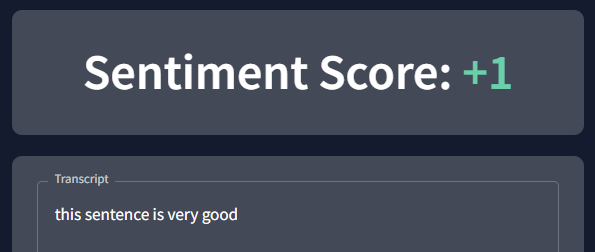
\includegraphics[scale=0.70]{images/sa1.png}
    \caption{Sentiment score computed using the AFINN-165 lexicon}
    \label{fig:sa1}
\end{figure}

\begin{figure}[H]
    \centering
    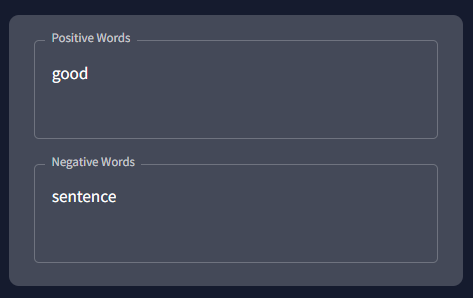
\includegraphics[scale=0.84]{images/sa2.png}
    \caption{Perceived positive and negative words using the AFINN-165 lexicon}
    \label{fig:sa2}
\end{figure}

Despite the weaknesses of the lexicon-based approach, its very high speed and efficiency makes it the most appropriate model to use in our real-time application, satisfying NFR.8 stated in Section \ref{nfrs}.

% Other approach discussing SA
% \paragraph{Selecting an Appropriate Model}

% In the third sprint of development, just after abandoning the backend-processing system architecture discussed in Section \ref{sysarch}, we decided to attempt to partially revert back to the backend-processing architecture, however, it would only conduct sentiment analysis and not process any frames. This was a more feasible alternative compared to using it for image processing as image transmission is a computationally expensive operation with high latency, whereas transmitting text is far more resource-friendly approach. The advantage of dedicating the backend purely for sentiment analysis was that Python has more libraries and tools available when it comes to NLP compared to JavaScript.

% Intially, in the third sprint pf development, we attempted to implement the backend-processing architecture just for the purposes of sentiment analysis. This was more feasible as text is far less computationally expensive to transmit than images, and hence the Flask python backend proposed earlier could use sentiment analysis models. The advantage of this approach was that python has more sentiment analysis models, ML models better. Here is a comparison. However, this in hindisght may have not been the best decision as despite text transmission being cheap, the frequency of it is high, as the text has to be transmitted everytime a word is spoken. Also models on the backend were too slow, despite being accurate, and hence violating NFR about our application being real-time. As a result a non-ML models were decided to be used. A sentiment library was used that uses AFINN etc.

% Compare SA models and methods
% 1. Using Text Blob
% 2. Using Vader
% 3. Using Bag of Words Vectorization-based Models
% 4. Using LSTM-based Models
% Using Transformer-based Models


\subsubsection{Facial Attribute Classification}

As established in Section \ref{ferrr}, deep learning models perform the best for image recognition tasks, such as FER, age recognition and sex recognition. Consequently, the pre-trained models we employed for our attribute classification tasks, were deep learning models implemented by a widely-used API for facial image recognition tasks called \textit{face-api.js} developed by \cite{faceapijs}. Face-api.js is a JavaScript API built on top of \textit{tensorflow.js}, which comes with several models to choose from for your image recognition task. We explain and evaluate each model we have used below for face detection, FER, age and sex recognition.

\paragraph{Face Detection}

For face detection, three models are offered by face-api.js:

\begin{itemize}
    \item \textbf{SSD Mobilenet V1} --- This is a neural network which implements a single-shot multibox detector (SSD) algorithm. It works by dividing the input image into multiple grids and predicting the presence of objects using a set of default bounding boxes and their offsets. As the SSD algorithm is a single-shot detection approach, it only requires a single forward pass through the neural network to make predictions, making it relatively fast and accurate. It will compute the locations of each face in an image and will return the bounding boxes together with it's probability for each face. This approach generally aims toward obtaining high accuracy in detecting face bounding boxes instead of low inference time; with the size of the quantised model being approximately 5.4 megabytes. The implementation of this model has been trained and tested on the WIDER FACE dataset previously discussed in Section \ref{facedet}, achieving a strong, but not quite state-of-the-art, classification accuracy of 85.20\%.
    
    \item \textbf{Tiny Face Detector} --- Tiny Face Detector is a high-performance CNN that operates in real-time that has been trained on a custom dataset of approximately 14,000 images labelled with bounding boxes. It is more efficient in terms of speed, size and resource consumption compared to the \textit{SSD Mobilenet V1} face detector. Furthermore, it generally produces marginally better classification results than \textit{SSD Mobilenet V1} on larger faces, achieving 86.93\% on the WIDER FACE dataset, however, it is less effective when detecting smaller faces. This is compensated however, by the model being very fast and resource efficient, with the size of the quantised model being approximately 190 kilobytes.

    \item \textbf{MTCNN} --- MTCNN is an implementation of the model discussed in Section \ref{facedet} proposed by \cite{xiang2017joint}. Despite it achieving state-of-the-art classification results on datasets such as WIDER FACE and AFLW, it is very slow as it is involves three cascading CNNs. The model size is 2 megabytes.

\end{itemize}

Out of the three face detection models discussed above, \textit{Tiny Face Detector} was chosen due to its speed and small size, hence being the most suitable for real-time applications, while still maintaining a good classification accuracy.

\paragraph{Attribute Classification}

For attribute classification, face-api.js offers two deep learning models, namely, \textit{faceExpressionNet} and \textit{ageGenderNet}. \textit{faceExpressionNet} is a CNN that classifies the face in an image into the emotion categories defined by \cite{ekman} and a neutral emotion category. It has been trained on multiple datasets including FER-2013 and AffectNet, achieving classification accuracies of 86.42\% and 82.56\% respectively. These accuracies are sufficient for our purposes, as we are not looking to necessarily use the most accurate model, but rather one that achieves similar results to contemporary models as stated by NFR.11 in Section \ref{nfrs}. Furthermore, faceExpressionNet is only 310 kilobytes, meaning it is very resource efficient and suitable for our real-time application. 
\np
The model offered by face-api.js for detecting age and sex is \textit{ageGenderNet}. This model uses a CNN architecture called VGG-19, shown in Figure \ref{fig:vgg}, which consists of 19 convolutional layers. The model has been trained on the \textit{`Asian Face Age Dataset'}, AFAD. The model, compared to contemporary models, achieves a strong accuracy of 97.01\% for predicting sex and a mean absolute error of 3.67 for predicting age on the AFAD dataset. 
\np
\begin{figure}[H]
    \centering
    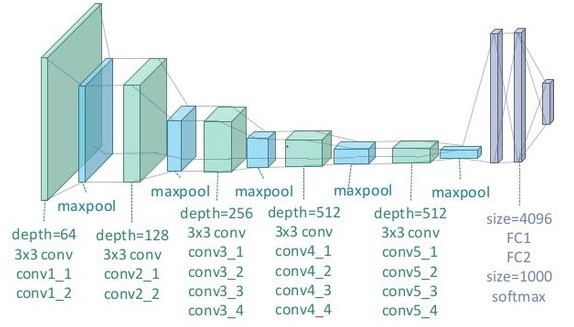
\includegraphics[scale=0.72]{images/vgg.jpg}
    \caption{VGG-19 neural network, a standard CNN architecture consisting of 19 convolutional layers, taken from \cite{vgg}}
    \label{fig:vgg}
\end{figure}

\paragraph{Using Attribute Models}

As shown in Figure \ref{fig:mvc} in Appendix \ref{appendix:sad}, when the user clicks the start button, i.e. a user event occurs, a state variable is changed, which is listened to using a \verb+useEffect+ hook. The function ran by the \verb+useEffect+ hook is the \verb+loadModels()+ function shown in Figure \ref{fig:codefer}.

\begin{figure}[H]
    \centering
    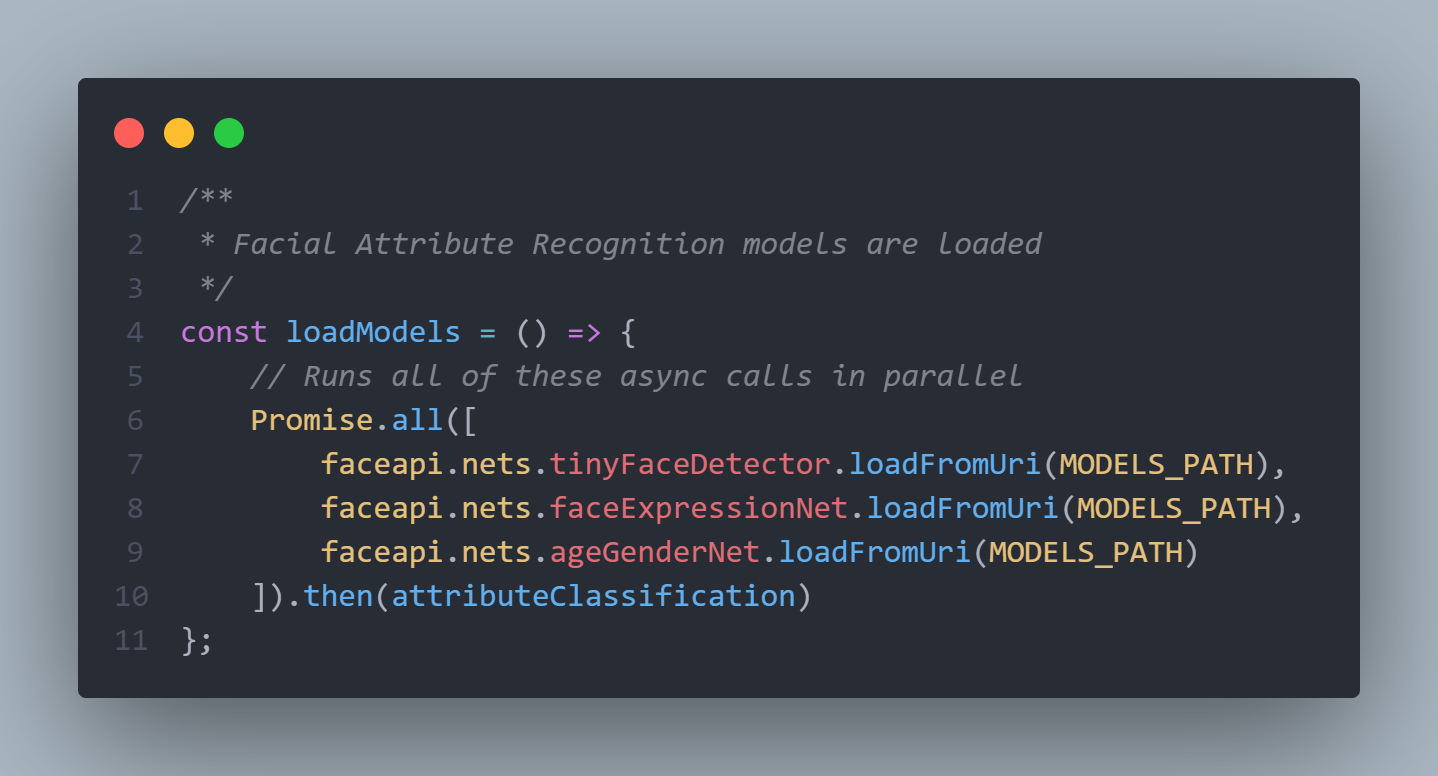
\includegraphics[scale=0.28]{images/codefer.png}
    \caption{Image showing how each pre-trained model is loaded}
    \label{fig:codefer}
\end{figure}


Lines 7-9 in Figure \ref{fig:codefer} show how the face detection model, \verb+tinyFaceDetector+, the FER model, \verb+faceExpressionNet+ and the age and sex model, \verb+ageGenderNet+ are loaded. As loading pre-trained models is not an instantaneous operation, and hence is an asynchronous task, promises are used so that the execution of the program is not blocked. In JavaScript, a \textit{promise} is an object that represents the eventual completion, or failure, of an asynchronous operation. Line 6 in Figure \ref{fig:codefer} shows how the \verb+Promise.all()+ function is used so that multiple asynchronous calls can be made in parallel, saving the user time and offering a more fluid experience. JavaScript's \verb+then()+ method is then used to handle the fulfilment of a promise object. In line 10 of Figure \ref{fig:codefer}, the function address of \verb+attributeClassification+ is given as an arguement to \verb+then()+ so that once the models have finished loading, attribute classification can begin.
\np

\begin{figure}[H]
    \centering
    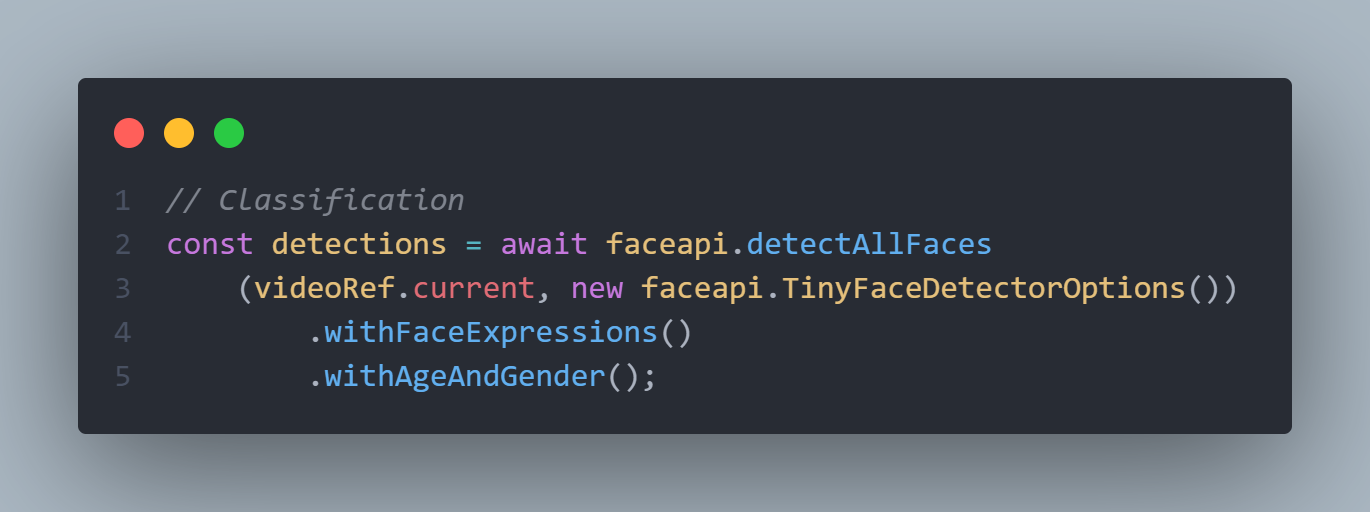
\includegraphics[scale=0.3]{images/codeferclassification.png}
    \caption{Code snippet of a part of the \textit{attributeClassification} function showing how the models are used to classify attributes}
    \label{fig:codeferclassification}
\end{figure}

Figure \ref{fig:codeferclassification} shows how once the \verb+tinyFaceDetector+ model has detected a face, we then run the FER, age and sex model. The JavaScript keyword \verb+await+ is used as the attribute models require a face to be found before classifying, which is an asynchronous operation, and hence we must wait for the promise of finding a face to be fulfilled, i.e. we must wait for the \verb+detectAllFaces()+ function to finish executing before resuming with the program. \verb+videoRef.current+ is given as input to the \verb+detectAllFaces()+ function as it is a reference to the user's webcam video stream element in the DOM.


\subsubsection{Lighting Conditions}

In this section, we will discuss the implementation of how our web application manages to gauge lighting conditions which was a low priority feature, as stated by FR.11 in Section \ref{frs}, and hence little research was done into existing approaches, as it was proposed as an extension to our application and doesn't form an important part of it. As a lot of computational burden is already put on the user's device due to the pre-traned models being used by the web application, we attempted to find a computationally inexpensive method of gauging lighting conditions. The two most common approaches involve calculating the \textit{luminance} of each pixel or alternatively, the \textit{perceived brightness}. In order to calculate perceived brightness, luminance must first be calculated, and is hence a more computationally expensive method and was therefore not chosen. Luminance is a linear measure of light, whereas perceived brightness is not. 
\np
In order to gauge the brightness of the lighting conditions of the user's webcam, we first must be able to retrieve the RGB, red-green-blue, colour values of each pixel in the webcam's current frame. This was done by drawing a canvas HTML element on top of the webcam window in the page, so rather than retrieving the frame directly from the webcam, we obtain it via the graphical, webcam window rendered on the page itself. After we have retrieved the frame's RGB values for each pixel, we then compute the luminance of the image by summing the luminance of each pixel in the canvas, and dividing it by the number of pixels in the image to form an average. The luminance of a pixel can be calculated using Equation \ref{eq:luminance}, where $L$ is the calculated luminance of the pixel and $R$, $G$, and $B$ are the red, green and blue colour channels of the pixel, respectively.

\begin{equation}
    L = 0.2126R + 0.7152G + 0.0722B\label{eq:luminance}
\end{equation}

If the average luminance of the image is greater than a pre-defined threshold, which we define as \verb+BRIGHTNESS_THRESH+ in the code, then we can determine whether the user has sufficiently bright lighting conditions. The code snippet for how luminance is calculated is shown in Figure \ref{fig:codeluminance} in Appendix \ref{appendix:codesnippets}.

\subsubsection{UI Implementation}
\label{uii}

As discussed and justified in Section \ref{uidesign}, the two main design principles we adopted were the Gestalt laws of perceptual organisation \citep{todorovic2008gestalt} and Nielsen's usability principles \citep{nielsen1994usability}. In this section, we discuss how these principles were implemented. Some examples of how the principles were implemented are as follows:

\begin{itemize}
    \item \textbf{Gestalt similarity principle} --- This principle states that we as human beings assume that if two things look similar, then their functionality will be similar; form informs function. One of the ways this principle was implemented for our application, was in the context of colour. Red is usually used in design for terminal features, such as `STOP', `END' or `CANCEL', whereas green is usually employed to initiate something, for example, `GO', `START' and `BEGIN' \citep{colley2021exploring}. The `START' button was made to be green, and the `STOP' button was made to be red, so the user, from previous experience of using other applications, is assisted in the process of determining the functions of the button by being able to map the functionality of green buttons they have seen in their past experience. 
    
    \begin{figure}[H]
        \centering
        
\includegraphics[scale=1]{images/ui-start.png}
        \caption{RTHAA's `START' button}
        \label{fig:ui-start}
    \end{figure}

    \begin{figure}[H]
        \centering
        
\includegraphics[scale=1]{images/ui-stop}
        \caption{RTHAA's `STOP' button}
        \label{fig:ui-stop}
    \end{figure}

    \item \textbf{Gestalt proximity principle} --- This principle states that if we see objects close together, we assume that they must be related. Figure \ref{fig:ui-proximity-components} shows how UI components associated with speech, are grouped on the left side of the UI, while the components associated with facial data, i.e. emotion, sex, etc. are grouped on the right side of the UI. Furthermore, \ref{fig:ui-proximity-buttons} shows how related buttons are grouped together. Buttons to do with high-level actions, such as logging the collected data or toggling the colour theme are placed together in the header, while buttons to do with the actual processing of data are grouped together at the centre of the UI, below the webcam window.
    
    \begin{figure}[H]
        \centering
        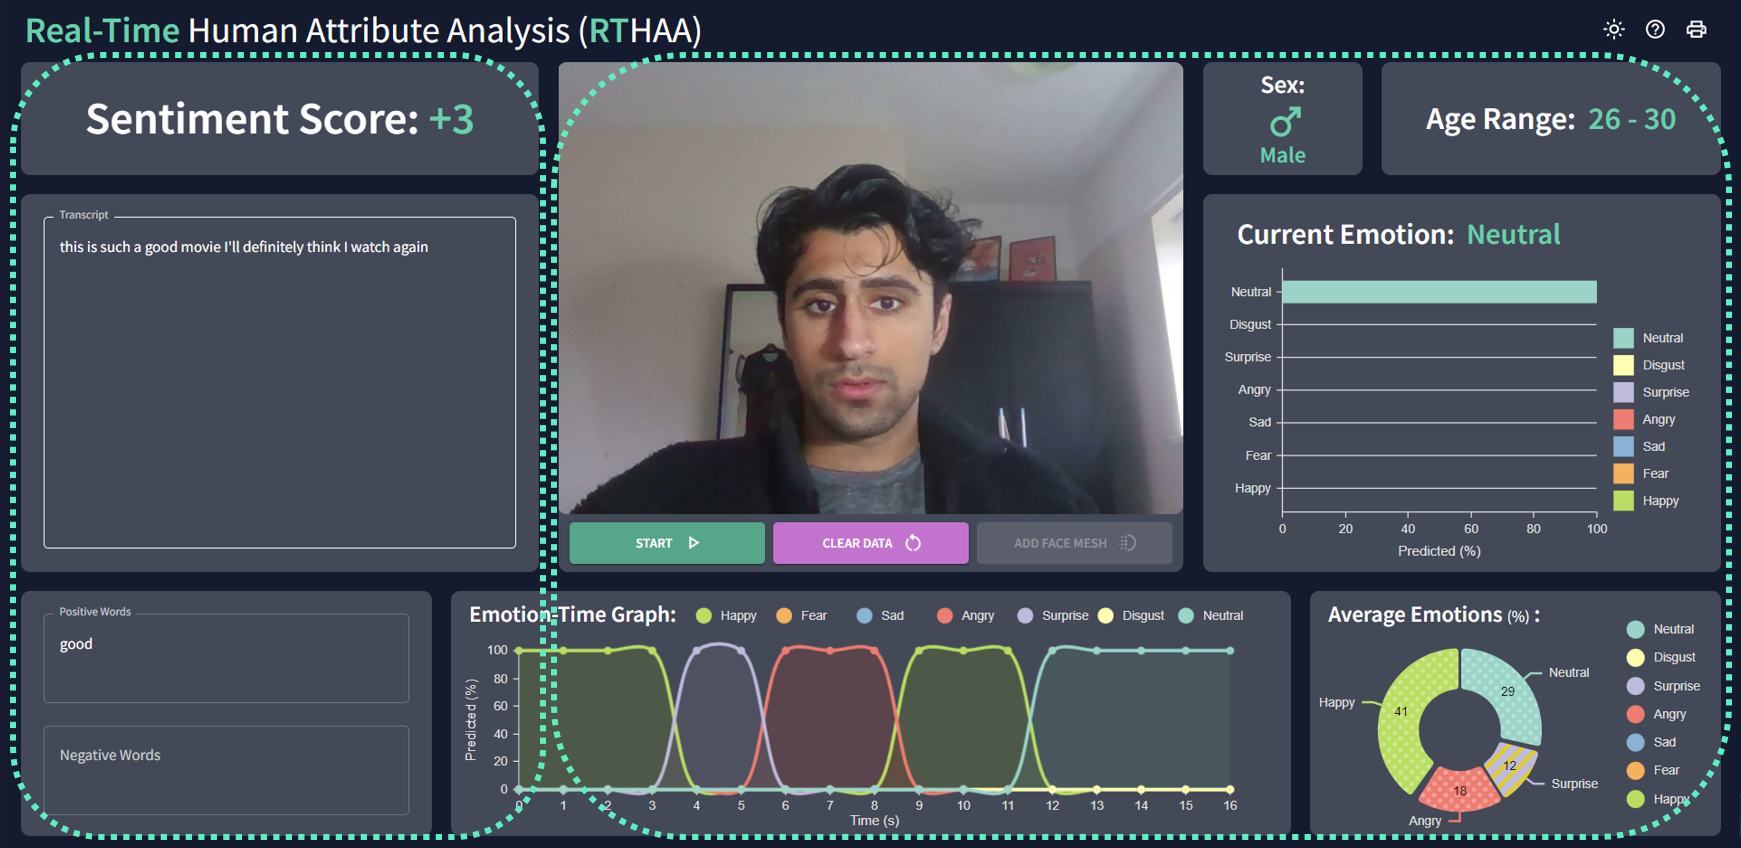
\includegraphics[scale=0.34]{images/ui-proximity-components.png}
        \caption{Screenshot of RTHAA outlining how related components are grouped together, specifically, components related to speech and components related to facial data, such as emotion and age}
        \label{fig:ui-proximity-components}
    \end{figure}

    \begin{figure}[H]
        \centering
        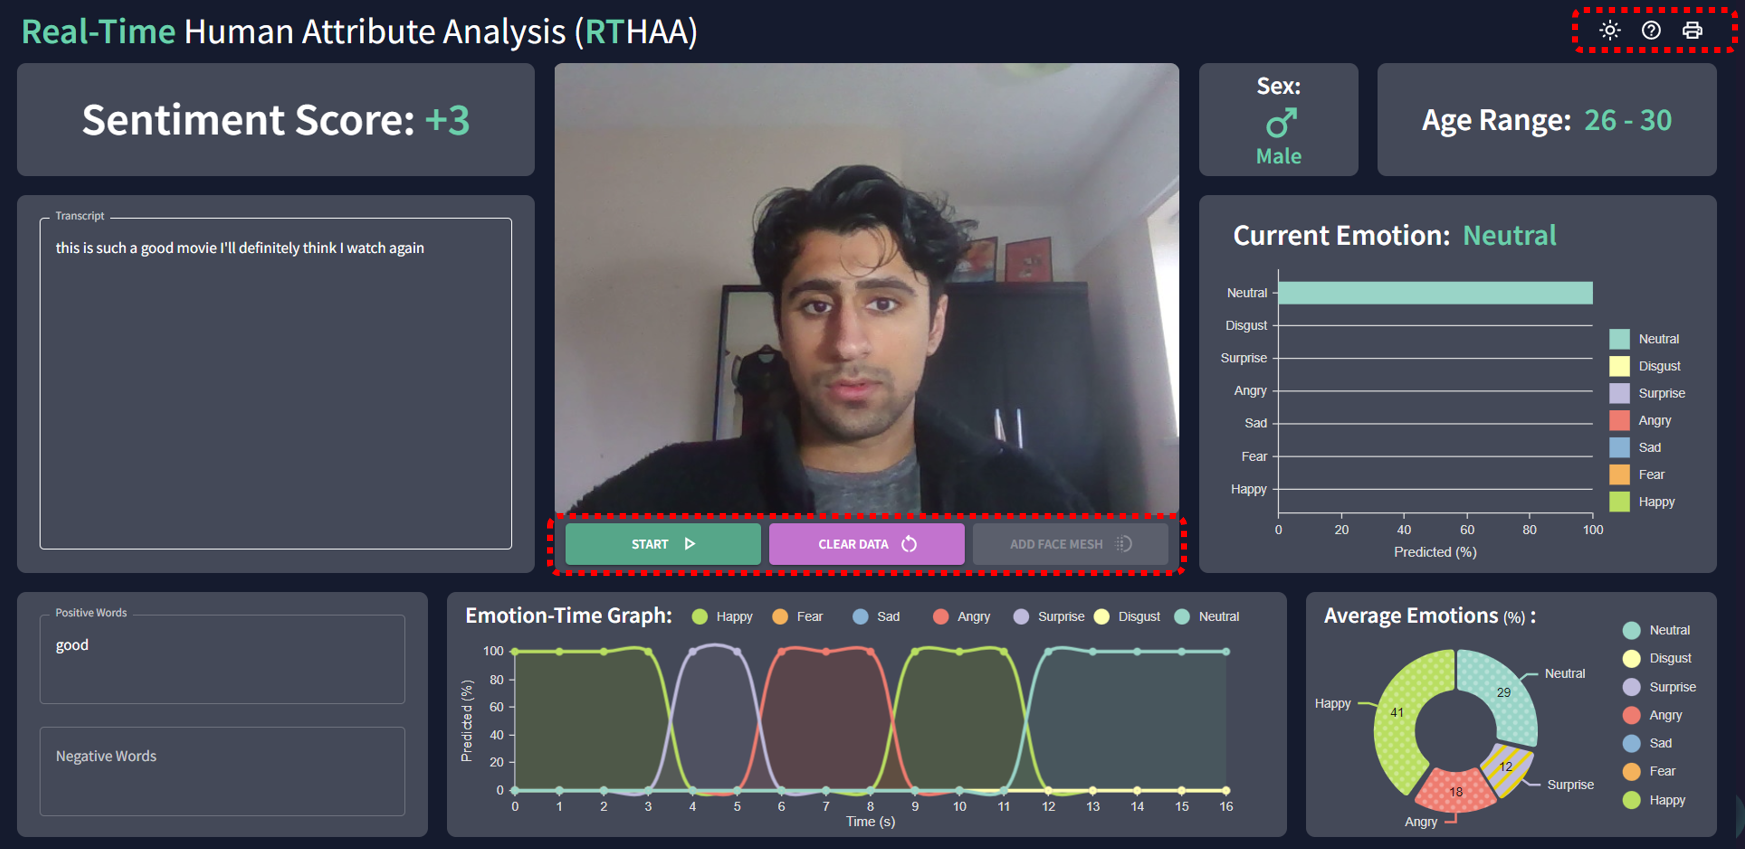
\includegraphics[scale=0.34]{images/ui-proximity-buttons.png}
        \caption{Screenshot of RTHAA outlining how related buttons are grouped together}
        \label{fig:ui-proximity-buttons}
    \end{figure}

    \item \textbf{Nielsen's `visibility of system status' principle} --- This principle emphasies the importance of keeping users informed of the status of the system. One way we have implemented this principle, is through the use of the `START' button. As opposed to having two separate `START' and `STOP' buttons, we employ the use of one button, which changes upon clicking, i.e. when the `START' button is clicked, the button itself changes to become the `STOP' button, informing the user that the application has started processing data.
    
    \item \textbf{Nielsen's `match between the system and real-world' principle} --- Similar to the Gestalt similatiry principle, this principle states how we as humans tend to map things from the system to the real-world. In this case, we use specific colours related to certain emotions, for example, in the real-world, red is often associated with anger, and consequently red is used for displaying `anger' on all data visualization components in the UI. Conversely, green is used for `happy'.
    
    \item \textbf{Nielsen's icon design principles} --- Icons were used to assist the user in determining the functionality of certain buttons. Figure \ref{fig:sun} shows how symbolism, i.e. a high-level abstraction, was used as the icon for toggling the light and dark theme of the page, represented by a sun to indicate brightness. Figure \ref{fig:print} uses an analogous image, in this case, the button prints the collected user data and hence we use a printer icon.
    

    \begin{figure}[H]
        \centering
        
\includegraphics[scale=0.30]{images/icon-sun.png}
        \caption{Toggle light/dark theme button}
        \label{fig:sun}
    \end{figure}


    \begin{figure}[H]
        \centering
        
\includegraphics[scale=0.20]{images/icon-print.png}
        \caption{Print collected user data button}
        \label{fig:print}
    \end{figure}

\end{itemize}

% UI: 
    % UI design - wcag compliance, colour palette, usability principles + gestalt etc. include loads of ss
    % Outline many drafts of UI design - state how it will be improved with each sprint as we incorporate user feedback
    % At the top is a header which has the name of the application, \textit{RTHAA}, and three buttons that are for the more higher-level options

    % We implemented each principle as follows:
    % Data visualization components themselves were made to be multi-coloured to help distinguish between different emotion classes, for example, green corresponds to happy, while red corresponds to anger. Certain coloured parts were also made to be textured to increase visibility and ultimately accessibility. This came from user testing which found that when the application was in light mode, the colour for disgust was hard to distinguish from the background.

    % \begin{figure}[H]
    %     \centering
    %     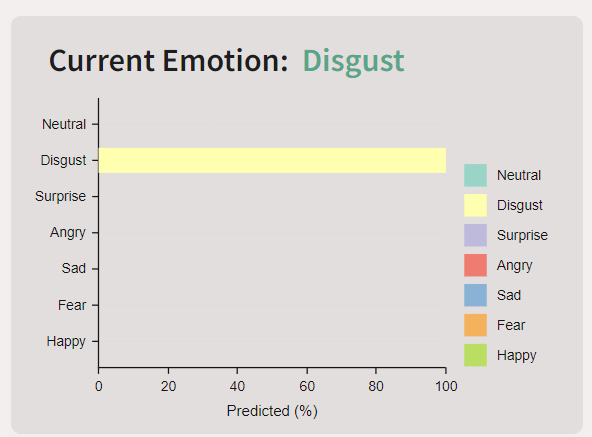
\includegraphics[scale=0.70]{images/disgustbefore.png}
    %     \caption{Current emotion component of \textit{RTHAA} showing the colour of disgust before texturing}
    %     \label{fig:disgustbefore}
    % \end{figure}

    % \begin{figure}[H]
    %     \centering
    %     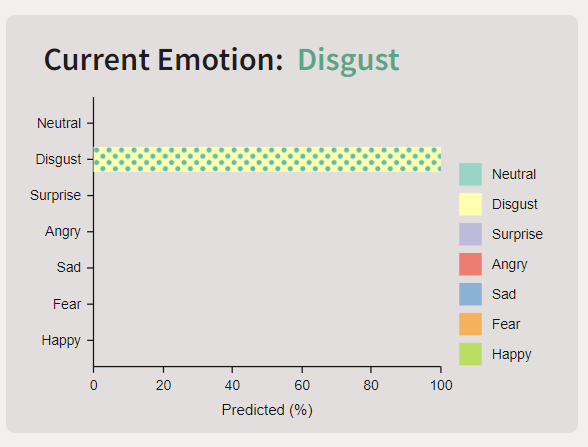
\includegraphics[scale=0.70]{images/disgustafter.png}
    %     \caption{Current emotion component of \textit{RTHAA} showing the colour of disgust after texturing, improving visibility}
    %     \label{fig:disgustafter}
    % \end{figure}

\clearpage
\section{Testing}
\label{testing}

As mentioned in Section \ref{sdm}, TDD was not employed since this is an individual project, and our tests are subject to the same bias as our application code. However, other forms of testing were conducted and will be discussed in this section.

\subsection{Unit Testing}
\label{ut}

Unit testing helps to identify defects early in the development cycle by isolating problems before they become conflated with other pieces of code. Unit testing was conducted by thoroughly testing individual React.js components, such as each data visualization component. As previously mentioned in Section \ref{finalimp}, components inherit props from parent components. Therefore, when it came to unit testing an individual component, the behaviour of the component was validated by testing it on all possible states of the props that it inherits. After the unit tests written for components were passed, the component would then be integrated into the application, allowing for integration testing to be conducted on higher-level components to see how multiple components interact with each other. This was done via the same method as unit testing; all possible values for a prop would be inputted into parent components, and these props would trickle down to their child components enabling us to assess the behaviour of the interaction between components.
\np
Throughout this project, unit testing was done on many of the pre-trained models and methods before employing them into the application. One example of such testing, was comparing the accuracy of different sentiment analysis models in Python. We compared two models, one which uses a lexicon, called \textit{VADER}, and one which uses machine learning, called \textit{RoBERTa}. Figure \ref{fig:sacomparison} shows the performance of the two models on the \textit{`Amazon Fine Food Reviews'} dataset, a common benchmark dataset used in sentiment analysis. The output of each model consists of three normalised values that indicate the degree of positivity, negativity, or neutrality of the input text. The test, shown in Figure \ref{fig:sacomparison}, concluded that the \textit{RoBERTa} pre-trained model performs better as it classifies each data point more accurately, compared to the \textit{VADER} model.

\begin{figure}[H]
    \centering
    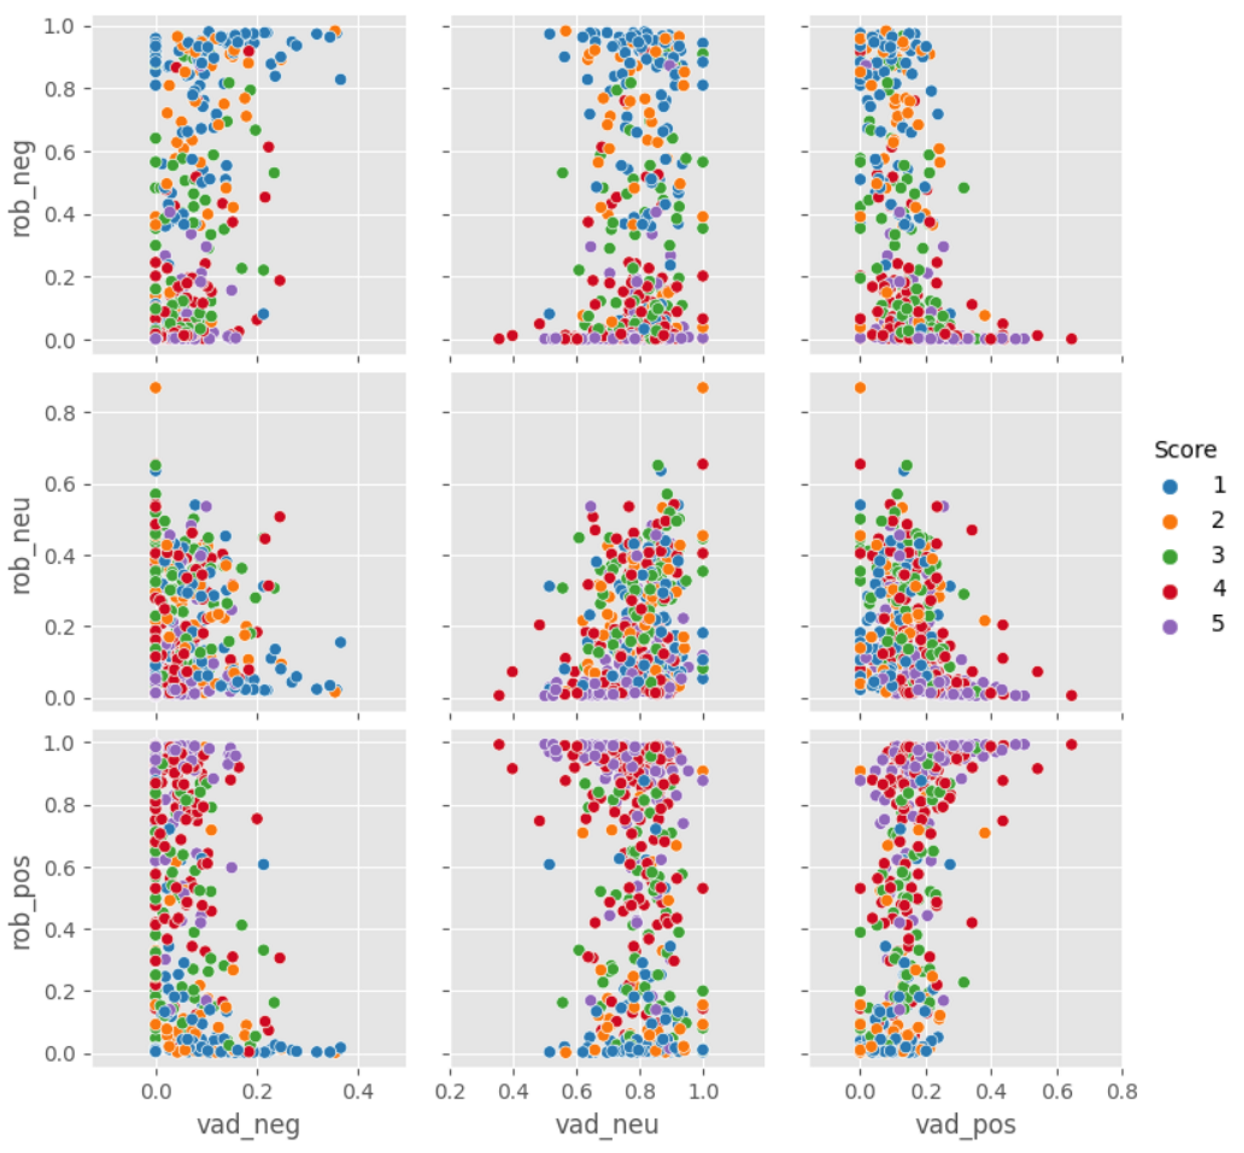
\includegraphics[scale=0.50]{images/sacomparison.png}
    \caption{Performance of VADER model (x-axis) compared to RoBERTa model (y-axis) on the \textit{`Amazon Fine Food Reviews'} dataset}
    \label{fig:sacomparison}
\end{figure}

\subsection{User Testing}
% Browser testing

User testing is important as it provides valuable feedback on how users interact with our application. Observing these interactions enables us to gain insights into user behavior, and make informed decisions on how to improve the user experience. Alpha testing methods were adopted in order to help detect defects in the application early on in the development process. One such example, was when the supervisor for this project identified that the webcam window should be horizontally inverted for a better user experience, so that user movements are more intuitively shown. Furthermore, the supervisor also stated that the contrast of colours in certain buttons should be changed to improve visibility.
\np
Beta testing methods were also employed towards the end of the project as the main features of the application were developed. In the penultimate sprint, a user, who was red-green colour-blind, stated that the coloured lines on the data visualization components were ``impossible to distinguish'' in light mode. Consequently, the line colours were updated to a more distinct set of colours, allowing for them to be more distinguishable in light mode, as shown in Figure \ref{fig:colourblind}. Figure \ref{fig:nocolourblind} shows the view for a user who is not colour-blind. Data visualization components were also made to have hover features, so that when the user hovers on them, a small box of text appears displaying what data they're hovering over. 

\begin{figure}[H]
    \centering
    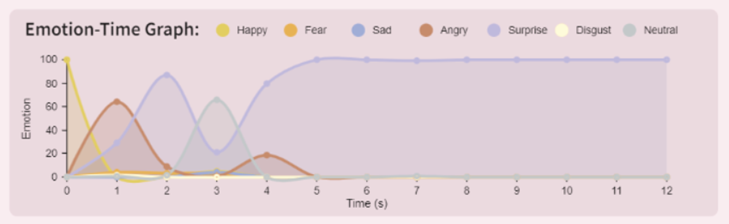
\includegraphics[scale=0.80]{images/colourblind.png}
    \caption{Updated view of the \textit{`EmotionTime'} component, where line colours are more distinguishable for a user who has deuteranomaly, a type of red-green colour-blindness}
    \label{fig:colourblind}
\end{figure}

\begin{figure}[H]
    \centering
    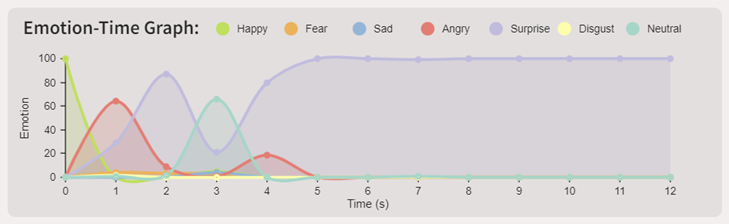
\includegraphics[scale=0.80]{images/nocolourblind.png}
    \caption{Updated view of the \textit{`EmotionTime'} component for a user who is not colour-blind, i.e. a trichromatic view}
    \label{fig:nocolourblind}
\end{figure}

User testing after each sprint allowed us to ensure that the final application offers a positive, accessible user experience. As a result, we managed to achieve an `A' conformance level to the WCAG2.1 \citep{WCAG21} guidelines, where `AAA' is the highest level of accessibility, and `A' is the minimum level of accessibility expected for web content.
\clearpage

\section{Evaluation}

In this section, we evaluate the success of the project, based on how well we met the requirements stated in Section \ref{reqs}. Additionally, we also evaluate the success of the project by exploring the results of a survey conducted on 12 people who tested the final application, as well as the other contemporary applications discussed in Section \ref{es}.

\subsection{Requirements}

All functional requirements stated in Section \ref{frs}, including `Should's and `Could's, were able to be completed, whereas not all non-functional requirements, stated in Section \ref{nfrs}, were able to be completed, specifically NFR.14 and NFR.15. These two requirements were low priority `Could' requirements and therefore only have a minor impact on the success of the project. Consequently, by looking at how well we met the requirements, we can say this project was a huge success overall.

\subsection{Survey}

In order to further evaluate the success of the project, a survey was conducted on 12 people who tested RTHAA, Noldus, MorphCast and iMotions. This evaluation method was chosen because surveys allows us to gauge the performance of more subjective aspects of the project, such as overall user experience. Care was taken to ensure that a diverse pool of participants were selected to mitigate the impact of any bias a particular group may have. This involved selecting participants of various ages, sexes and ethnicities. Since most of the participants selected were close friends or family, care was taken to ensure participants weren't aware which application was which, to minimise any personal bias. Ideally, a larger pool of participants would be preferable and yield more accurate results. After participants used all four tools, they were given a survey containing the following questions:

\begin{enumerate}
    \item Which application do you feel best identified your attributes, i.e. how accurately did it predict your emotions, age and sex?

    \item Which application had the better user experience?    
    
    \item Which of the four applications do you prefer overall?

    \item What were the strengths and weaknesses of each application? Please elaborate.
\end{enumerate}

Figure \ref{fig:survey} shows the results of the survey for questions 1, 2 and 3. It clearly depicts RTHAA having a significantly superior user experience and being the most preferred application of the four. Furthermore, the results show that RTHAA was rated higher when it came to predicting the attributes of the participants. This is likely due to the significant amount of research and evaluation done into selecting appropriate pre-trained models, hence resulting in better performance, as well as RTHAA being multimodal and able to detect a wider range of human attributes compared to the other tools. 

\begin{figure}[H]
    \centering
    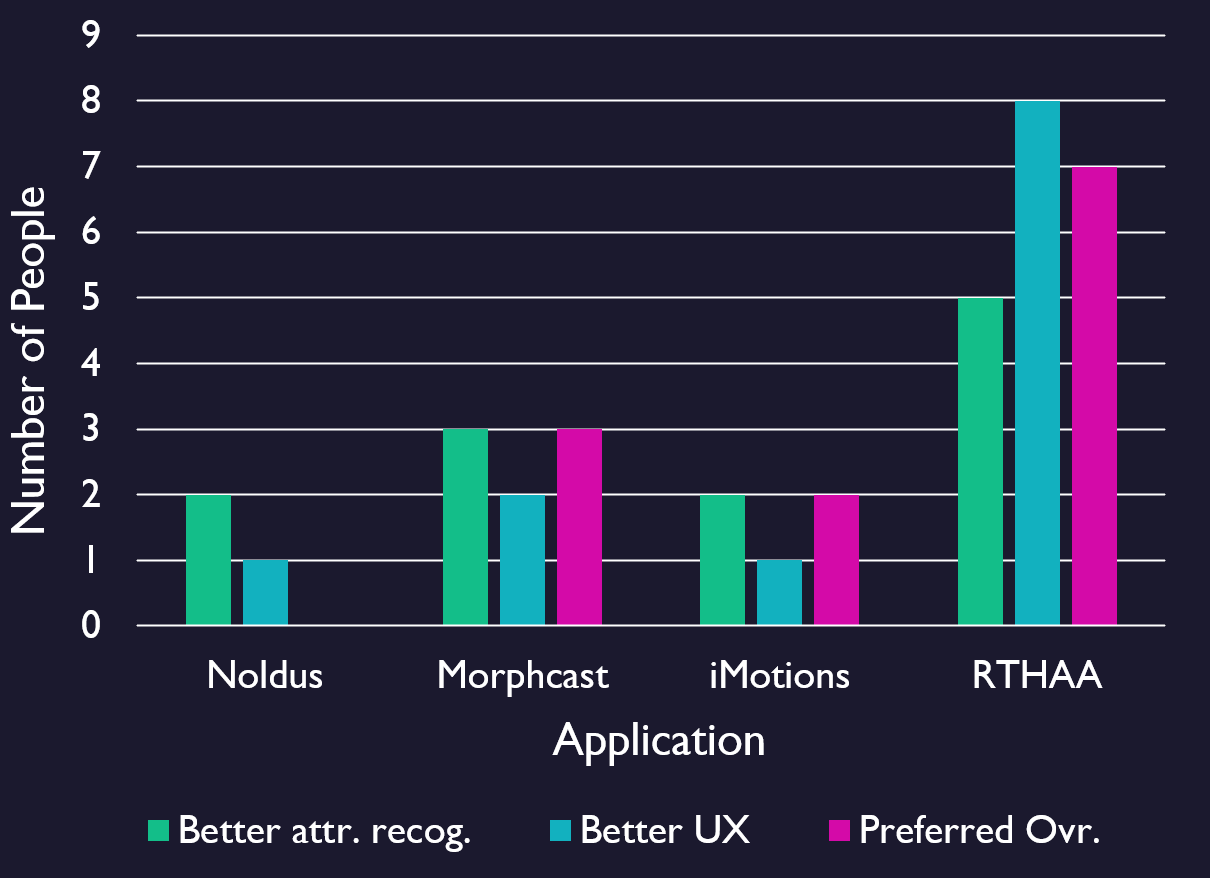
\includegraphics[scale=0.50]{images/survey.png}
    \caption{Results of the survey conducted on 12 participants}
    \label{fig:survey}
\end{figure}

The responses to question 4 relating to RTHAA complemented the accuracy of the FER model employed, as well as the age and sex model. However, some of the weaknesses stated by users were that the application could often misclassify the sentiment of certain words, however, the overall sentiment score was mostly correct. This was an issue, discussed in Section \ref{saam}, and is a fundamental issue of employing a lexicon-based model. One participant also stated that the predicted age would sometimes increase in response to a new facial expression. This is potentially due to certain expressions causing more wrinkling of the skin and hence causing the age model to predict a higher age, however, as only one participant said this, we cannot be sure if this is a persistent issue, once again showing how this survey would benefit from testing on more people. 

% Ideally more participants from a wider range of background, ages, etchnicites etc.

% Talk more in your final report about the participants chosen for the UI evaluation. Was it a mix of ages/genders/ethnicities?? If not, try to make sure you have a variety, but at the very least if this is not possible you should discuss it as a limitation.

% show that it picked up sarcasm "user testing showed that it picked up sarcasm"

\section{Conclusion and Future Work}


% To summarise, this project has successfully developed a web application capable of analysing user's emotions, speech sentiment, age, sex and lighting conditions so that businesses can better measure how 
% Furthermore, this application is unique in that it is the only application of its kind that is both multimodal and accessible for all to use on the internet, as well as it being the most comprehensive, providing auxillary features such as lighting detection.


To summarise, this project has successfully developed a well-designed web application, capable of analysing a person's emotions, speech sentiment and other attributes. Based on user testing, the application was found to provide a more accurate assessment of a user's system experience compared to existing tools. In addition, this application distinguishes itself as the only one of its kind that is both multimodal and accessible on the internet, requiring no installation of software. Moreover, it boasts a wide range of features, including auxiliary features like age, sex and lighting detection, making it the most comprehensive tool available. The final product is an intuitive, well-designed application which fulfils all of the core objectives outlined at the start of the project. Furthermore, there was a large research component to this project which delved into other methods of emotion recognition, such as through physiological signals. This project managed to overcome many unforseen challenges, most notably of which was switching architecture design late in development, from a backend-processing architecture to a frontend. Another difficulty this project entailed, was how many different areas of computer science it had to combine, namely, full-stack web development, machine learning, sentiment analysis and many more in order to develop the final application.
\np
The major lessons learned in this project mainly concern the tools employed. Various tools that are built on top of React.js could have been utilised to save development time, such as TypeScript, which provides a statically-typed interface to React.js. Redux could've also been employed to help state management in React.js.

\subsection{Future Work}
\label{fw}
As with any product, limitations are inevitable. In this section we discuss the limitations of the application and how it forms the basis for future work and improvement.
\np
One limitation of the application is the accuracy of the sentiment analysis model employed. As mentioned before, it uses a lexicon-based approach which has low classification accuracy, but is high speed. Possible future work could involve developing a model which uses a machine learning approach, but is still fast enough for real-time purposes. Another limitation of the application is that its speech recognition capability is not supported on non-chromium-based browsers, such as FireFox, meaning sentiment analysis cannot be conducted on the user's speech. This is due to the speech recognition library used, which is not natively supported by FireFox. Possible future work may involve solving this issue by using a polyfill, i.e. we host our own speech recognition service which implements the web speech API discussed in Section \ref{srecog} and therefore allows speech to be converted to text on non-chromium-based browsers.

% Reflection - USe typscript etc.

% Reflext at the end on the appropriateness of the approach and any changes you would suggest

\section{Ethical Considerations}
\label{lsepi}

Various potential ethical concerns were identified during the development of the application, the most notable of which was attempting ethnicity detection, i.e. we predict the user's ethnicity based off of their face. However, this feature was removed as it could warrant racially motivated behaviour. Furthermore, the model used for ethnicity detection has the risk of being biased, which could result in unfair or discriminatory outcomes. Privacy concerns were also raised when using the backend-processing architecture. Users may feel uneasy about sending their personal information, such as their age and sex, to a remote server where it could potentially be stored and misused if adequate safeguarding procedures are not implemented. Moreover, in accordance with the UK's Data Protection Act \citep{dpa}, which is the UK's implementation of the General Data Protection Regulation (GDPR), obtaining user consent would be necessary for storing this information. Additionally, complete transparency regarding the processing of the data would also be required.


\section{Author's Assessment of the Project}

\begin{itemize}
    \item What is the (technical) contribution of this project?
    \np
    This project contributes a well-designed web application, capable of analysing a person's emotions, speech sentiment and other attributes. Based on user testing, the application was found to provide a more accurate assessment of a user's system experience compared to existing tools. In addition, this application distinguishes itself as the only one of its kind that is both multimodal and accessible on the internet, requiring no installation of software. Moreover, it boasts a wide range of features, including auxiliary features like age, sex and lighting detection, making it the most comprehensive tool available.

    \item Why should this contribution be considered relevant and important for the subject of your degree?
    \np
    This project's contribution should be considered important as it paves the way for businesses to be able to test their products more scalably and accurately, by analysing the user experience of their customers. The applications scalability comes from it being a web application, available to anyone with an internet connection and a browser. User testing also showed that it gauges user experience more accurately than existing solutions.

    \item How can others make use of the work in this project?
    \np
    Others can use this project's software output not only for their own use, but also as a basis for creating even more advanced human attribute analysis tools, which gauge user experience using even more modalities, models and methods. 

    \item Why should this project be considered an achievement?
    \np
    This project should be considered an achievement not only because all core requirements were fulfilled, but more importantly, because it genuinely improves upon existing tools that are available for analysing human attributes.  
    
    \item What are the limitations of this project?
    \np
    As discussed in Section \ref{fw}, the model used for sentiment analysis could be improved as the users in our survey highlighted this as a weakness of the application, so perhaps it is worth using a slower, more accurate model instead. Furthermore, while the application is supported on many popular browsers such as Google Chrome, Microsoft Edge and Safari, its speech-to-text feature is not supported on non-chromium-based browsers, such as FireFox, meaning sentiment analysis cannot be conducted on the user's speech on those particular browsers.

\end{itemize}

% Based on user testing, the application was found to provide a more accurate assessment of a user's system experience compared to existing tools. In addition, this application distinguishes itself as the only one of its kind that is both multimodal and accessible on the internet, requiring no installation of software. Moreover, it boasts a wide range of features, including auxiliary features like age, sex and lighting detection, making it the most comprehensive tool available. The final product is an intuitive, well-designed application which fulfils all of the core objectives outlined at the start of the project. Furthermore, there was a large research component to this project which delved into other methods of emotion recognition, such as through physiological signals. This project managed to overcome many unforseen challenges, most notably of which was switching architecture design from a backend-processing architecture to a frontend. Another difficulty of this project was how many different areas of computer science had to be combined, namely, web development, machine learning, sentiment analysis and many more.

% Brought together many areas of comp sci

%  Mention that you were given no technical assistance, and how this project was done completely on your own

\clearpage
\addcontentsline{toc}{section}{References}		% Add references to table of contents

\bibliographystyle{agsm}						
% Harvard referencing: agsm
% Ordered referencing: unsrt
% Plain referencing: plain
% Plain Natbib referencing: \bibliographystyle{./common/plainnat}  % MAKE SURE TO ADD FOLDER contiaining natbib
\bibliography{bibliography}

\begin{appendices}
\pagestyle{fancy}
\lhead{Neema Raiyat}											    % LHS of header
\rhead{Real-time Human Attribute Analysis Web App}                  % RHS of header


\section{Existing Solutions Screenshots}
\label{appendix:ess}

\begin{figure}[H]
    \centering
    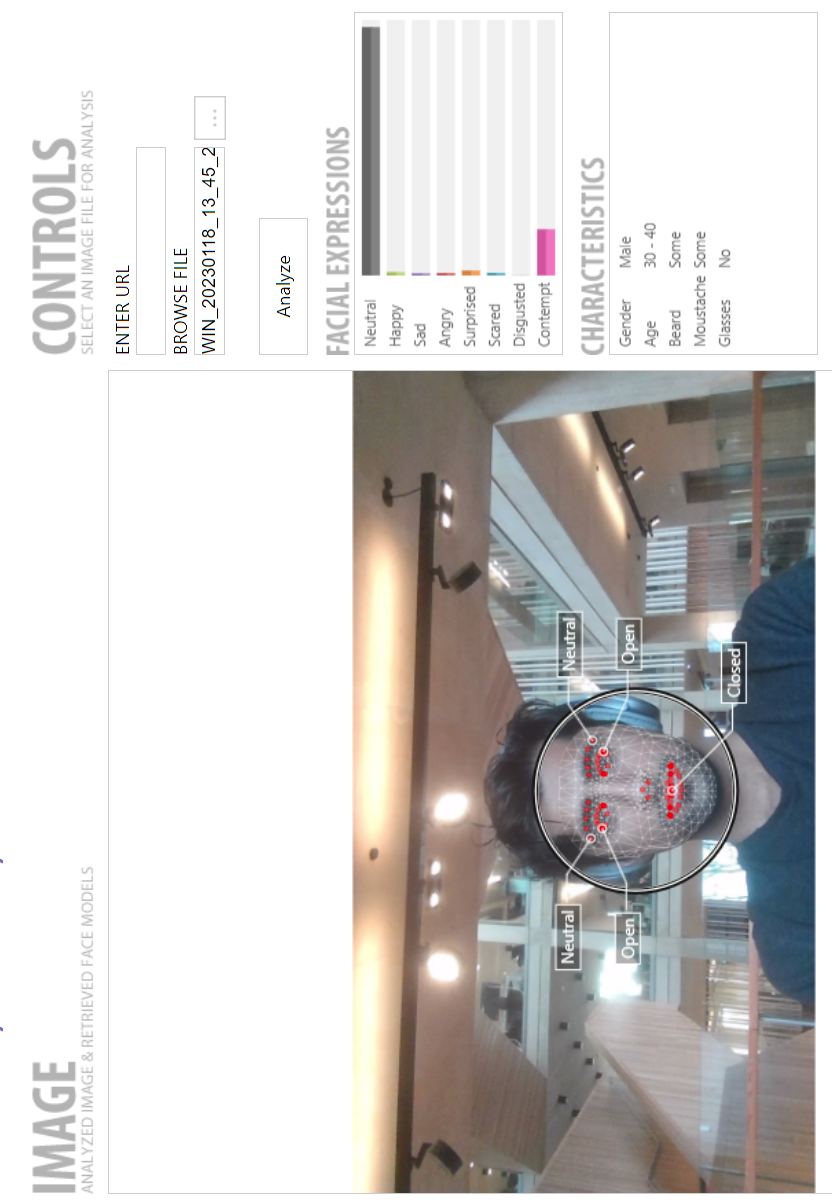
\includegraphics[scale=0.76]{images/noldus.png}
    \caption{A screenshot of \cite{noldus}}
    \label{fig:essnoldus}
\end{figure}

\begin{figure}[H]
    \centering
    \includegraphics[scale=0.43]{images/morphcast.png}
    \caption{A screenshot of \cite{morphcast}}
    \label{fig:essmorphcast}
\end{figure}

\begin{figure}[H]
    \centering
    \includegraphics[scale=0.48]{images/imotions.png}
    \caption{A screenshot of \cite{imotions}}
    \label{fig:essimotions}
\end{figure}
\section{Project Methodology Screenshots}
\label{appendix:pmss}

\subsection{Kanban Board}
\label{appendix:kanban}

\begin{figure}[H]
    \centering
    \includegraphics[scale=0.57]{images/kanban.png}
    \caption{A screenshot of the kanban board used in this project}
    \label{fig:kanbanss}
\end{figure}

\subsection{Gantt Charts}
\label{appendix:ganttcharts}

\begin{figure}[H]
    \centering
    \includegraphics[scale=0.55]{images/gantt1.png}
    \caption{Gantt chart showing the planned schedule of the project}
    \label{fig:gantt1}
\end{figure}

\begin{figure}[H]
    \centering
    \includegraphics[scale=0.58]{images/gantt2.png}
    \caption{Gantt chart showing the executed timeline of the project}
    \label{fig:gantt2}
\end{figure}

\section{System Diagrams}
\label{appendix:sad}

\begin{figure}[H]
    \centering
    \addtolength{\leftskip} {-2cm}
    \addtolength{\rightskip}{-2cm}
    \includegraphics[scale=0.53]{diagrams/sa1.png}
    \caption{System architecture diagram showing key components of architecture that uses a remote server}
    \label{fig:febe}
\end{figure}

\begin{figure}[H]
    \centering
    \includegraphics[scale=0.50]{diagrams/sa2.png}
    \caption{System architecture diagram showing key components of architecture that processes all data in the frontend}
    \label{fig:allfe}
\end{figure}

\begin{figure}[H]
    \centering
    \includegraphics[scale=0.72]{diagrams/MVC.png}
    \caption{Simplified diagram showing how the MVC architectural pattern was implemented in \textit{RTHAA}}
    \label{fig:mvc}
\end{figure}

\section{Application Screenshots}
\label{appendix:ass}

\begin{figure}[H]
    \centering
    \includegraphics[scale=0.53]{images/webapp1.png}
    \caption{MVP 1 of RTHAA dashboard}
    \label{fig:wa1}
\end{figure}

\begin{figure}[H]
    \centering
    \includegraphics[scale=0.45]{images/webapp4.png}
    \caption{MVP 2 of RTHAA dashboard}
    \label{fig:wa3}
\end{figure}

\begin{figure}[H]
    \centering
    \includegraphics[scale=0.58]{images/webappFE3.png}
    \caption{MVP 3 of RTHAA dashboard, using face-api.js}
    \label{fig:wa4}
\end{figure}

% \begin{figure}[H]
%     \centering
%     \includegraphics[scale=0.58]{images/webappFE6.png}
%     \caption{MVP 4 of  of RTHAA dashboard}
%     \label{fig:wa5}
% \end{figure}

\begin{figure}[H]
    \centering
    \includegraphics[scale=0.58]{images/webappFE7.png}
    \caption{MVP 4 of RTHAA dashboard}
    \label{fig:wa6}
\end{figure}

\begin{figure}[H]
    \centering
    \includegraphics[scale=0.58]{images/webappFE10.png}
    \caption{MVP 5 ofRTHAA dashboard}
    \label{fig:wa7}
\end{figure}

\begin{figure}[H]
    \centering
    \includegraphics[scale=0.58]{images/webappFE12.png}
    \caption{Finished RTHAA dashboard in light mode}
    \label{fig:wa8}
\end{figure}

\begin{figure}[H]
    \centering
    \includegraphics[scale=0.58]{images/webappFE13.png}
    \caption{Finished RTHAA dashboard in dark mode}
    \label{fig:wa9}
\end{figure}

\section{Code Snippets}
\label{appendix:codesnippets}

\begin{figure}[H]
    \centering
    \includegraphics[scale=0.31]{images/codeluminance.png}
    \caption{Code snippet showing how the lighting conditions of the user are determined}
    \label{fig:codeluminance}
\end{figure}

\end{appendices}
\end{document}